\chapter{降维}
\label{chap:dimensionality-reduction}

基因测量或文档向量可以包含成千上万个坐标，其中许多坐标却描述相近的变化。若能用较少的数值保留分析所需的信息，后续计算和解释就更容易展开。\term{降维}（dimensionality reduction）把观测$\bm{x}\in\mathbb{R}^{d}$转为表示$\bm{z}\in\mathbb{R}^{k}$，通常取$k\ll d$。压缩时需要先决定保留什么：方差、点间距离、邻域关系和生成因素各有用途，对后续预测、分组或解释的价值也需要分别检验。

降维方法的发展也围绕这些不同的保留目标展开。20世纪初的PCA提取线性变化的主要方向，1950年代的MDS根据对象差异恢复坐标。1990年代的核PCA将方差分析带入非线性特征空间，2000年前后的Isomap与LLE从局部关系组织几何表示；2008年的t-SNE和2018年的UMAP则扩展了高维邻域的可视化方法\scite{dimScholkopf1998,dimTenenbaum2000}

在压缩、去噪和建模前处理时，PCA可以作为简单基线；探索局部邻域时，t-SNE与UMAP常用来安排便于观察的坐标。图上的分离提示了值得检验的关系，检验仍要使用原始表示和任务证据\scite{classic-decomposition-guide,dim-mcinnes2018umapsoftware}本章沿保留的信息展开：从线性组合及核特征中的全局变化，转向点间差异和局部关系，再讨论如何用低维因素解释观测的生成。

为比较这些方法，以下用$n$表示样本数，$\bm{X}\in\mathbb{R}^{n\times d}$与$\bm{Z}\in\mathbb{R}^{n\times k}$按行存放观测和低维表示，邻居数记为$q$，内在维数记为$m$。“表示”是变换结果的统称；几何或邻域坐标称为“嵌入”；参与生成但未被观测的量称为“潜变量”。第\ref{chap:classic-models-overview}章的共享建模机制为这些不同目标提供了共同背景。

\section{基于线性关系的降维}
\label{sec:dim-linear}

多个传感器若主要随同一个物理量变化，观测可能集中在一条直线附近；多个共同因素则可以对应一个低维线性子空间。线性投影$\bm{z}=\bm{W}^{\top}(\bm{x}-\bm{\mu})$提取沿该子空间的坐标，其中$\bm{W}\in\mathbb{R}^{d\times k}$为列正交的基矩阵，$\bm{\mu}$为中心，$\bm{W}\bm{W}^{\top}$是相应的正交投影算子。方向学得后，矩阵乘法就能编码新样本，每个坐标也对应原特征的一个线性组合。

线性组合还可以用于重构，而不要求编码是输入的线性函数。非负矩阵分解和稀疏编码都用基向量组合观测，新样本的系数却通常由约束优化取得；独立源分离还要使用协方差以外的统计信息。核PCA保留的则是核所定义的特征空间中的方差。因此，本节会分别说明线性关系作用于编码、生成还是映射后的特征，再据此判断各方法保留的信息与求解方式。

\subsection{主成分分析（PCA）}
\label{sec:dim-pca}

一个投影方向可以按两种准则选择：投影后留下的变化有多大，由投影恢复原样本的平方误差有多小。\term{主成分分析}（principal component analysis, PCA）在正交投影设定下把两者联系起来：方差最大的方向张成平均平方重构误差最小的子空间。Pearson在1901年研究点集的最佳拟合直线与平面，Hotelling在1933年研究多元统计中的主成分，分别从几何拟合与变量变化说明了这一结构\scite{pearson1901pca,hotelling1933pca}

\subsubsection{模型结构}
\label{sec:dim-pca-structure}

比较投影方差之前，需要把共同中心与样本变化分开。减去样本均值后，暂以$\bm{X}$表示中心化数据，样本协方差为$\bm{S}=\bm{X}^{\top}\bm{X}/n$。分母$n$与最大似然的协方差约定一致；使用$n-1$会统一缩放特征值，主成分方向保持相同。

单位方向$\bm{w}$上的投影方差为$\bm{w}^{\top}\bm{S}\bm{w}$。为同时保留$k$个互相正交的变化方向，将它们组成$\bm{W}$，最大化这$k$个坐标的方差总和：
\begin{equation}
  \max_{\bm{W}^{\top}\bm{W}=\bm{I}_k}
      \operatorname{tr}(\bm{W}^{\top}\bm{S}\bm{W}),
  \qquad \bm{Z}=\bm{X}\bm{W}.
  \label{eq:dim-pca-variance}
\end{equation}
约束使$\bm{W}$的列构成候选$k$维子空间的一组正交基，迹目标衡量该子空间保留的总方差。这里比较的是子空间，每一列尚未规定为协方差特征向量。编码得到的得分$\bm{z}=\bm{W}^{\top}\bm{x}$则是样本在这组基下的坐标。

把得分沿基向量组合起来，重构为$\widehat{\bm{x}}=\bm{W}\bm{W}^{\top}\bm{x}$。原样本由投影与正交残差组成，勾股关系因而给出
\begin{equation}
  \lVert\bm{x}-\widehat{\bm{x}}\rVert_2^2
  =\lVert\bm{x}\rVert_2^2-\lVert\bm{W}^{\top}\bm{x}\rVert_2^2.
  \label{eq:dim-pca-pythagoras}
\end{equation}
对全部样本取平均时，右侧第一项与$\bm{W}$无关，第二项就是保留的总方差。因此，增大投影方差等价于减小平均平方重构误差，图\ref{fig:dim-pca-projection}显示了这一分解。新观测编码时使用训练均值中心化，重构时再加回该均值。

\begin{figure}[htbp]
  \centering
  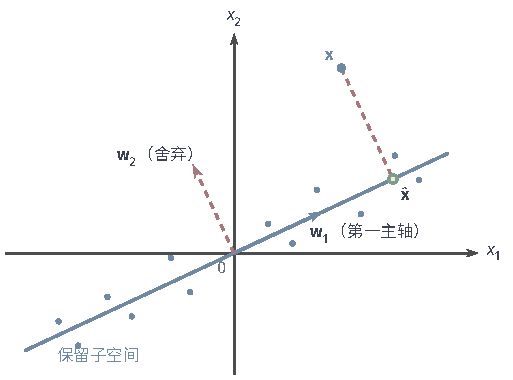
\includegraphics[width=86.935mm]{figures/04-classic-models/00-shared/tikz/dim-pca-projection/figure.pdf}
  \caption{二维到一维的正交投影示意。蓝色实线方向$\bm{w}_1$是保留的第一主轴，红色虚线方向$\bm{w}_2$是被舍弃的正交主轴。点$\bm{x}$投到$\widehat{\bm{x}}$，重构残差沿$\bm{w}_2$方向。图中散点为示意位置，未表示真实实验。}
  \label{fig:dim-pca-projection}
\end{figure}

\subsubsection{参数学习}
\label{sec:dim-pca-learning}

最优方向可以通过协方差的谱求出。在单位方向的约束目标中引入乘子$\lambda$，驻点方程为$\bm{S}\bm{w}=\lambda\bm{w}$，投影方差正好等于$\lambda$。按$\lambda_1\geq\cdots\geq\lambda_d\geq0$排序，前$k$个特征向量组成$\bm{V}_k$，其列称为\term{主成分方向}（principal component directions）。取$\bm{W}=\bm{V}_k$得到一个解析最优解；得分$\bm{X}\bm{V}_k$的经验协方差为$\operatorname{diag}(\lambda_1,\ldots,\lambda_k)$，所以这些得分不相关，统计独立还需要额外条件。

方向的唯一性需要分别看基矩阵、子空间与投影算子。一般最优$\bm{W}$是一组正交基，$\operatorname{span}(\bm{W})$是其张成的主子空间，$\bm{P}=\bm{W}\bm{W}^{\top}$是相应投影。若$\lambda_k>\lambda_{k+1}$，主子空间与投影唯一；子空间内部仍可以旋转，任意$k$阶正交矩阵$\bm{Q}$都使$\bm{W}\bm{Q}$给出同一投影，所有最优基可写成$\bm{V}_k\bm{Q}$。

坐标基的旋转却会改变各列及得分之间的关系。从$\bm{W}=\bm{V}_k$出发，若$\bm{Q}$混合不同特征值的方向，$\bm{W}\bm{Q}$的列一般不再是$\bm{S}$的特征向量，得分协方差$\bm{Q}^{\top}\operatorname{diag}(\lambda_1,\ldots,\lambda_k)\bm{Q}$一般也不再对角。因此，互不相关的主成分得分对应排序特征向量基$\bm{V}_k$，而非主子空间中的任意正交基。

如果进一步要求各列为排序后的特征向量，单特征值方向只差符号；所选范围内的重特征值允许在其重特征子空间中旋转。若$\lambda_k=\lambda_{k+1}$，重特征值跨过截断位置，最优主子空间和投影算子也可能不唯一。

实际计算通常对中心化数据作\term{奇异值分解}（singular value decomposition, SVD），写成$\bm{X}=\bm{U}\bm{\Sigma}\bm{V}^{\top}$。右奇异向量给出主方向，$\lambda_j=\sigma_j^2/n$，得分为$\bm{U}_k\bm{\Sigma}_k$。直接SVD无需显式形成$\bm{X}^{\top}\bm{X}$，可以避免条件数平方带来的数值困难。完整稠密分解约需$O(nd\min(n,d))$次运算，只求少数方向时还可使用截断算法；不同实现需要不同的矩阵和计算预算。

当$d\gg n$时，样本空间中的$n\times n$ Gram矩阵$\bm{X}\bm{X}^{\top}$更小。若$\bm{X}\bm{X}^{\top}\bm{u}_j=\sigma_j^2\bm{u}_j$且$\sigma_j>0$，右奇异向量可由$\bm{v}_j=\bm{X}^{\top}\bm{u}_j/\sigma_j$恢复。这仍是同一SVD；第\ref{sec:dim-kpca}节将沿样本空间计算引出核方法。

求出特征值后，可以衡量前$k$个方向保留的方差比例。\term{累计解释方差}（cumulative explained variance）定义为
\begin{equation}
  \eta_k=\frac{\sum_{j=1}^{k}\lambda_j}
                    {\sum_{j=1}^{d}\lambda_j}.
  \label{eq:dim-explained-variance}
\end{equation}
总方差非零时，可以按预先选择的比例确定$k$，也可以查看特征值随序号下降的碎石图。$85\%$、$95\%$等比例是经验阈值，并非预测信息的保证：低方差方向可能包含第\ref{sec:classification-lda-reduction}节的类别判别信息，高方差也可能来自量纲或背景干扰。是否标准化由特征单位和任务决定；服务于预测的维数选择应使用训练集内部的验证结果。

矩阵规模过大时，还可以近似求主子空间。随机化SVD先估计列空间，再分解较小的矩阵；增量PCA按批次更新子空间。二者以近似误差或特定更新规则换取内存与时间收益，评价时需要同时检查求解精度\scite{halko2011}

\subsubsection{理论分析}
\label{sec:dim-pca-theory}

\paragraph{表达能力}
PCA的候选表示由线性子空间限定，适合主要变化集中在该空间附近的数据。弯曲流形的变化可能无法由一个子空间保留，低方差中的任务信息也可能在截断时被删去。方差目标衡量重构中的变化量，预测价值则由具体任务决定。

\paragraph{收敛性}

固定数据上的最优重构可以由Eckart--Young低秩逼近定理说明\scite{eckart1936}下面将这一结果用于PCA的正交重构，再把它与估计总体子空间的问题分开。

在正交投影与平方误差设定下，前$k$维主子空间达到经验全局最优，最小误差等于舍弃特征值的总和。截断处的谱隙进一步决定投影是否唯一：

\begin{theorem}[PCA的最优线性重构性质]
  \label{thm:dim-pca-optimal}
  设$\bm{X}$已中心化，$1\leq k<d$，$\lambda_j$为$\bm{S}=\bm{X}^{\top}\bm{X}/n$按降序排列的特征值。则
  \[
    \min_{\bm{W}^{\top}\bm{W}=\bm{I}_k}
       \frac1n\lVert\bm{X}-\bm{X}\bm{W}\bm{W}^{\top}\rVert_F^2
       =\sum_{j=k+1}^{d}\lambda_j.
  \]
  前$k$个特征向量张成的子空间达到最小值。若$\lambda_k>\lambda_{k+1}$，最优投影算子$\bm{W}\bm{W}^{\top}$唯一，但子空间内的正交基不唯一。
\end{theorem}

\begin{proof}
在所有秩至多为$k$的矩阵中，截断SVD使平方Frobenius误差最小（参见\BookTheoremRef{thm:matrix-analysis-best-low-rank}{第一卷“数学准备”的Eckart--Young--Mirsky定理}）。
截断SVD给出$\bm X\bm V_k\bm V_k^\top$，其平方误差为$\sum_{j>k}\sigma_j^2$；
除以$n$并代入$\lambda_j=\sigma_j^2/n$即得结论。
截断处的严格谱隙使主子空间与投影唯一，唯一的投影仍允许在其子空间中选择不同的正交基。
\end{proof}

迭代谱算法要逼近的是定理中的全局最优投影，可以用特征方程残差和方向正交误差检查数值精度。增加迭代可以改善求解误差；样本是否足以估计总体结构，则是下面的统计问题。

\paragraph{泛化性}

训练样本上的最优平均重构还需要与总体风险比较。设总体中心为$\bm{0}$、协方差为$\bm{\Sigma}_{\star}$，秩$k$正交投影$\bm{P}$的总体重构风险为$R(\bm{P})=\operatorname{tr}((\bm{I}-\bm{P})\bm{\Sigma}_{\star})$。样本风险的最优投影记为$\widehat{\bm{P}}$，总体最优投影记为$\bm{P}_{\star}$；在两者风险差中加入并减去样本协方差项，可以得到
\begin{equation}
  \begin{aligned}
  R(\widehat{\bm{P}})-R(\bm{P}_{\star})
  &\leq\operatorname{tr}
      ((\bm{P}_{\star}-\widehat{\bm{P}})
        (\bm{\Sigma}_{\star}-\bm{S}))\\
  &\leq 2k\lVert\bm{S}-\bm{\Sigma}_{\star}\rVert_2.
  \end{aligned}
  \label{eq:dim-pca-excess-risk}
\end{equation}
第一步由$\widehat{\bm{P}}$的经验最优性得到，第二步使用$\bm{P}_{\star}-\widehat{\bm{P}}$的核范数至多为$2k$；核范数是奇异值之和。若编码使用样本均值，总体风险还要计入均值估计误差。固定$d$、独立同分布且二阶矩有限时，均值与协方差依大数定律收敛，风险差随之趋零。方向估计对谱隙更敏感：相近特征值对应的方向可以明显旋转，重构误差却可能只改变很少。

维数与样本数同步增长时，需要使用相应的高维统计条件。Nadler在尖峰协方差模型中的分析表明，样本特征值和方向可能偏离总体结构，弱信号甚至无法一致识别\scite{nadler2008}Marchenko--Pastur型谱极限提供了一个噪声基准：独立同分布噪声且$d/n$趋于正常数时，即使总体协方差为单位矩阵，样本特征值仍形成非退化的极限谱分布\scite{marchenko1967}该结论依赖具体矩阵模型与比例极限，修正样本谱时也需要这些条件。

高维估计可以利用不同结构限制。稀疏PCA减少活跃载荷，奇异值阈值或收缩则调整谱幅度，例如用于低秩矩阵去噪。Donoho与Gavish的最优硬阈值依赖指定噪声与损失条件，选择修正方式时应先核对其统计模型\scite{donoho2014threshold}

\subsubsection{支持稀疏载荷（Sparse PCA）}
\label{sec:dim-sparse-pca}

主成分若由几乎所有特征组成，很难从载荷看出哪些变量共同驱动一个方向。\term{稀疏PCA}（sparse PCA）限制载荷中的非零项，使一个成分主要由少数变量表达。Zou、Hastie与Tibshirani在2006年用回归式矩阵分解把成分提取与变量选择结合，并讨论基因表达等高维数据\scite{zou2006spca}稀疏要求直接参与优化，而非在普通PCA求解后再删除较小载荷：
\begin{equation}
  \begin{aligned}
  \min_{\bm{A},\bm{B}}\quad&
    \lVert\bm{X}-\bm{X}\bm{B}\bm{A}^{\top}\rVert_F^2
    +\lambda_1\sum_{j=1}^{k}\lVert\bm{b}_j\rVert_1
    +\lambda_2\lVert\bm{B}\rVert_F^2,\\
  \text{约束}\quad&\bm{A}^{\top}\bm{A}=\bm{I}_k.
  \end{aligned}
  \label{eq:dim-sparse-pca}
\end{equation}
在此目标中，$\bm{A},\bm{B}\in\mathbb{R}^{d\times k}$，$\bm{b}_j$是$\bm{B}$第$j$列，$\lambda_1,\lambda_2\geq0$。$\bm{B}$给出编码载荷，$\bm{A}$给出重构方向；$\ell_1$惩罚促使载荷稀疏，平方惩罚缓解相关变量造成的数值不稳定。

交替求解时，固定$\bm{A}$，可以将$\bm{X}$分到$\bm{A}$的列空间与正交补：
\[
  \lVert\bm{X}-\bm{X}\bm{B}\bm{A}^{\top}\rVert_F^2
  =\lVert\bm{X}\bm{A}-\bm{X}\bm{B}\rVert_F^2
   +\lVert\bm{X}(\bm{I}-\bm{A}\bm{A}^{\top})\rVert_F^2.
\]
第二项与$\bm{B}$无关，所以编码载荷可以按列求弹性网回归。转而固定$\bm{B}$，需要最大化$\operatorname{tr}(\bm{A}^{\top}\bm{X}^{\top}\bm{X}\bm{B})$，这是寻找最佳正交对齐的Procrustes问题，可由SVD求解。交替更新通常得到局部解，初始化与惩罚强度的敏感性需要检查。

稀疏载荷让变量组合更容易辨认，同时也改变了得分之间的关系。$\bm{B}$各列通常不正交，得分方差可能重叠，因此各成分方差之和不能直接作为标准PCA式的解释方差。基因表达和文本等应用需要同时评价稀疏程度、重构效果与跨样本稳定性。

\subsubsection{支持异常值与低秩加稀疏分解（Robust PCA）}
\label{sec:dim-robust-pca}

稀疏PCA限制使用的变量，异常值处理则需要改变误差模型。幅度很大的污染会在平方误差中占据较大权重；固定摄像机视频的低变化背景与少数变化像素提供了一个例子。把视频帧排为观测矩阵$\bm{M}\in\mathbb{R}^{n\times d}$，可尝试分解成低秩背景$\bm{L}$与稀疏扰动$\bm{E}$。这里的\term{鲁棒PCA}（robust PCA, RPCA）专指低秩加稀疏分解，稳健子空间估计还包括其他污染设定。

同时寻找低秩部分和稀疏部分时，直接最小化$\operatorname{rank}(\bm{L})+\lambda\lVert\bm{E}\rVert_0$存在组合困难。\term{主成分追踪}（principal component pursuit, PCP）用两个凸惩罚替代秩和非零元素数：
\begin{equation}
  \min_{\bm{L},\bm{E}}\
     \lVert\bm{L}\rVert_*+\lambda\lVert\bm{E}\rVert_1,
  \qquad \bm{M}=\bm{L}+\bm{E}.
  \label{eq:dim-pcp}
\end{equation}
核范数$\lVert\bm{L}\rVert_*=\sum_j\sigma_j(\bm{L})$鼓励较少的非零奇异值；$\lVert\bm{E}\rVert_1$为所有元素绝对值之和，鼓励较少的非零污染项。两个惩罚分别作用于整体秩结构与逐元素扰动。

分解能否恢复真实两部分，关键在于它们是否可区分。一个既低秩又稀疏的矩阵可以在$\bm{L}$与$\bm{E}$之间转移，造成歧义。Candès等的精确恢复定理要求低秩部分不相干，即奇异向量不集中在少数坐标，还限制秩、污染比例与随机支持。在这些条件下，$\lambda=1/\sqrt{\max(n,d)}$无需预先知道污染幅度；任意位置的对抗污染仍需另查是否符合条件\scite{candes2011rpca}

两个惩罚可以由\term{交替方向乘子法}（alternating direction method of multipliers, ADMM）分开求解，再通过重构约束协调。取惩罚参数$\rho>0$，引入与$\bm{M}$同形的$\bm{U}$作为缩放对偶变量，即拉格朗日乘子除以$\rho$。固定$\bm{U}$并略去无关常数，增广目标为
\[
  \lVert\bm{L}\rVert_*+\lambda\lVert\bm{E}\rVert_1
  +\frac{\rho}{2}
   \lVert\bm{M}-\bm{L}-\bm{E}+\bm{U}\rVert_F^2.
\]
固定$\bm{E}$更新$\bm{L}$，再用新$\bm{L}$更新$\bm{E}$，分别对应两种阈值运算。随后将尚未满足的重构误差加到$\bm{U}$，让下一轮继续校正约束偏差。从$\bm{U}^{(0)}=\bm{0}$开始时，一轮更新为
\begin{equation}
  \begin{aligned}
  \bm{L}^{(t+1)}&=\operatorname{SVT}_{1/\rho}
                  (\bm{M}-\bm{E}^{(t)}+\bm{U}^{(t)}),\\
  \bm{E}^{(t+1)}&=\mathcal{S}_{\lambda/\rho}
                  (\bm{M}-\bm{L}^{(t+1)}+\bm{U}^{(t)}),\\
  \bm{U}^{(t+1)}&=\bm{U}^{(t)}
                   +\bm{M}-\bm{L}^{(t+1)}-\bm{E}^{(t+1)}.
  \end{aligned}
  \label{eq:dim-rpca-admm}
\end{equation}
逐元素软阈值为$\mathcal{S}_{a}(u)=\operatorname{sign}(u)(|u|-a)_+$，$\operatorname{SVT}_{a}$则将同一运算作用于奇异值。模型中的$\bm{E}$代表稀疏扰动，迭代中的$\bm{U}$累积重构约束误差。为检查固定$\rho$下的停止条件，需要同时计算
\[
  \begin{aligned}
    r_{\mathrm{pri}}^{(t+1)}
      &=\lVert\bm{M}-\bm{L}^{(t+1)}-\bm{E}^{(t+1)}\rVert_F,\\
    r_{\mathrm{dual}}^{(t+1)}
      &=\rho\lVert\bm{E}^{(t+1)}-\bm{E}^{(t)}\rVert_F.
  \end{aligned}
\]
原始残差检查重构等式，对偶残差检查第二个子问题的变化是否仍破坏前一个子问题的平衡。两项均应低于按数据尺度设置的容差；迭代次数只是预算，不能代替这两项检查。

小幅稠密噪声可通过$\lVert\bm{M}-\bm{L}-\bm{E}\rVert_F\leq\delta$的稳定PCP约束容纳。在线变体处理流式观测，侧信息变体利用已知子空间特征。视频背景、遮挡或异常检测中的污染需要与所选模型对应；例如整行异常更适合组稀疏惩罚，逐元素稀疏并不描述同一种结构。

\subsubsection{小结}
\label{sec:dim-pca-summary}

PCA在给定数据上得到平均平方误差最小的正交线性压缩，并提供共享的编码与重构。所得子空间受维数、尺度和异常值影响，总体估计又受样本量与谱隙影响。稀疏PCA约束载荷，RPCA描述污染，第\ref{sec:dim-ppca}节的概率PCA描述噪声与潜变量；这些扩展需要按各自改变的假设选择。

\subsection{典型相关分析（CCA）}
\label{sec:dim-cca}

一张图像和对应文字使用不同坐标，却可以描述共同内容。分别保留两侧最大方差，可能先保留各自独有的变化。\term{典型相关分析}（canonical correlation analysis, CCA）让成对观测分别投影，再选择对应得分相关系数最大的方向，从而提取共同变化。Hotelling的经典工作建立了这一双视图分析框架\scite{hotelling1936cca}

\subsubsection{模型结构}
\label{sec:dim-cca-structure}

将成对观测中心化，记$\bm{x}\in\mathbb{R}^{d_x}$、$\bm{y}\in\mathbb{R}^{d_y}$，两侧协方差为$\bm{\Sigma}_{xx}$、$\bm{\Sigma}_{yy}$，交叉协方差为$\bm{\Sigma}_{xy}=\mathbb{E}[\bm{x}\bm{y}^{\top}]$。用同一批配对样本估计这些矩阵后，第一对方向按投影相关系数选择：
\begin{equation}
  \max_{\bm{w}_x,\bm{w}_y}
  \frac{\bm{w}_x^{\top}\bm{\Sigma}_{xy}\bm{w}_y}
  {\sqrt{\bm{w}_x^{\top}\bm{\Sigma}_{xx}\bm{w}_x}
   \sqrt{\bm{w}_y^{\top}\bm{\Sigma}_{yy}\bm{w}_y}}.
  \label{eq:dim-cca-correlation}
\end{equation}
相关系数只有在两侧投影方差均非零时有定义。缩放方向不改变相关性，因此可以令两侧方差均为$1$，将求解转为最大化交叉协方差。

图\ref{fig:dim-cca-shared}用两个视图比较方差与共有信息。各自方差最大的坐标$u$、$v$相互独立，较小方差的坐标却同为$t$，所以PCA与CCA会选择不同方向。此比较保留原坐标的方差；逐坐标标准化改变方差结构，也会改变PCA选择。

\begin{figure*}[!ht]
  \centering
  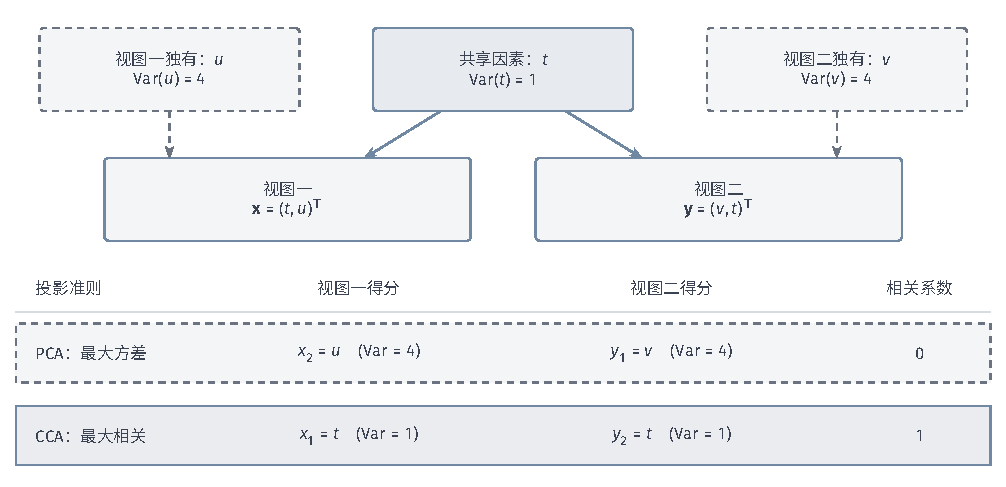
\includegraphics[width=169.000mm]{figures/04-classic-models/00-shared/tikz/dim-cca-shared/figure.pdf}
  \caption{CCA提取共有变化的构造例子。设$t,u,v$相互独立且均值为零，方差依次为$1,4,4$；两视图为$\bm{x}=(t,u)^\top$和$\bm{y}=(v,t)^\top$。实线连接共享因素，虚线连接各视图独有因素。各保留一维时，PCA选择$u,v$，CCA选择$t,t$，对应相关系数分别为$0$和$1$。箭头表示坐标构造关系，图中结论针对给定总体，不是样本拟合结果。}
  \label{fig:dim-cca-shared}
\end{figure*}

提取多对得分时，要求同一视图内$\bm{W}_x^{\top}\bm{\Sigma}_{xx}\bm{W}_x=\bm{I}_k$、$\bm{W}_y^{\top}\bm{\Sigma}_{yy}\bm{W}_y=\bm{I}_k$，使各得分方差为一且互不相关。这是协方差度量下的正交，原坐标中的方向未必欧氏正交。跨视图得分协方差可对角化为$\operatorname{diag}(\rho_1,\ldots,\rho_k)$，可识别的方向对数则同时受维数、样本秩与交叉协方差秩限制。

\subsubsection{参数学习}
\label{sec:dim-cca-learning}

两侧协方差正定时，可以先白化，使每侧协方差变成单位阵。白化后的交叉协方差及其SVD为
\[
  \bm{K}=\bm{\Sigma}_{xx}^{-1/2}
               \bm{\Sigma}_{xy}\bm{\Sigma}_{yy}^{-1/2},
  \qquad
  \bm{K}=\bm{U}\bm{D}\bm{V}^{\top}.
\]
令$\bm{a}=\bm{\Sigma}_{xx}^{1/2}\bm{w}_x$、$\bm{b}=\bm{\Sigma}_{yy}^{1/2}\bm{w}_y$，方差约束成为单位范数约束，目标成为$\max\bm{a}^{\top}\bm{K}\bm{b}$。取$\bm{K}$的首对左右奇异向量，就达到最大奇异值；多对方向由相应奇异向量依次取得：
\begin{equation}
  \bm{W}_x=\bm{\Sigma}_{xx}^{-1/2}\bm{U}_k,\qquad
  \bm{W}_y=\bm{\Sigma}_{yy}^{-1/2}\bm{V}_k,
  \label{eq:dim-cca-svd}
\end{equation}
$\bm{D}$的前$k$个对角元给出典型相关系数。实现白化时，可以使用Cholesky分解和三角求解，避免显式形成逆矩阵。

这一求解也可写成广义特征值问题。约束驻点满足$\bm{\Sigma}_{xy}\bm{w}_y=\rho\bm{\Sigma}_{xx}\bm{w}_x$及另一侧的对称方程，消去$\bm{w}_y$后得到
\[
  \bm{\Sigma}_{xy}\bm{\Sigma}_{yy}^{-1}
       \bm{\Sigma}_{yx}\bm{w}_x
  =\rho^2\bm{\Sigma}_{xx}\bm{w}_x.
\]
样本协方差奇异时，可只在非零方差子空间中求解，或分别加$\lambda_x\bm{I}$、$\lambda_y\bm{I}$进行正则化。正则化改变了归一化度量，训练相关系数因而需要配合留出配对样本的相关性一起评价。

共有变化也可以在非线性特征中寻找。核CCA固定核映射后匹配相关性，深度CCA则直接学习两侧变换\scite{andrew2013dcca}Andrew等2013年的方法通过两条联合训练的参数映射保留相关性目标，让新样本以前向计算获得表示。这改变了固定核的表示限制与样本展开方式，同时增加了需要控制的模型复杂度。

\subsubsection{小结}
\label{sec:dim-cca-summary}

CCA以共有线性变化组织配对传感器、多模态匹配或跨域表示，目标是相关性。某一视图独有却重要的信息可能未被保留，相关性也需要额外假设才能作因果解释。高维小样本容易高估训练相关性，应通过正则化与样本外配对检验控制这一问题。双塔表示和对比学习也对齐多视图，但各自的负采样、损失与训练规则需要另外说明。

\subsection{独立成分分析（ICA）}
\label{sec:dim-ica}

协方差为零只能排除线性相关。例如$X\sim\mathcal{N}(0,1)$时，$X$与$X^2$的协方差为零，后者却完全由前者确定。混合的多个源信号若要彼此分离，需要进一步利用分布中的依赖。\term{独立成分分析}（independent component analysis, ICA）据此结合源独立性与非高斯结构估计混合过程，用于说话人分离、脑电活动分析和眼动伪迹分离等任务\scite{comon1994ica}

信息论提供了另一种减少分量依赖的准则。Bell与Sejnowski在1995年研究非线性网络中的信息传递，推导出利用协方差以外统计信息的学习规则，并讨论未知混合语音的分离和未知回声的消除\scite{bell1995infomax}这类问题称为盲信号处理，因为混合或传播过程未知；对源信号的结构仍需作出假设。

\subsubsection{模型结构}
\label{sec:dim-ica-structure}

为说明解混关系，先取中心化、无噪声且源数等于观测通道数的模型：
\begin{equation}
  \bm{x}=\bm{A}\bm{s},\qquad
  \bm{z}=\bm{W}^{\top}\bm{x},\qquad
  \bm{W}^{\top}=\bm{A}^{-1}.
  \label{eq:dim-ica-model}
\end{equation}
混合矩阵$\bm{A}\in\mathbb{R}^{d\times d}$可逆，源$\bm{s}$的分量相互独立。此处$\bm{W}$的列存放解混方向，所以$\bm{W}=\bm{A}^{-\top}$。若将$\bm{A}^{-1}$直接称为解混矩阵，则编码用它左乘观测；两种记法描述同一运算。

识别这些方向还要求源非退化，且至多一个源为高斯。多个标准高斯源的联合分布在正交旋转后相同，因而无法从观测辨认该子空间中的方向。源排列与尺度也存在歧义：交换源及混合列，或对两者作反向缩放，观测$\bm{x}$保持相同。

存在密度时，可以比较解混分量的联合分布与边际乘积，用KL散度衡量剩余依赖。写成熵的形式为
\[
  I(z_1,\ldots,z_d)
  =\sum_{j=1}^{d}h(z_j)-h(\bm{z}),
\]
$h$为微分熵，上式要求各项有定义；散度为零恰好对应分量独立。也可以在单位方差约束下寻找非高斯方向，例如最大化负熵$J(z)=h(g)-h(z)$，其中$g$与$z$均值、方差相同且服从高斯分布。独立量相加趋向高斯提供了分离的直觉，具体对比量在有限线性组合中的性质仍需检验，不能直接由中心极限定理得到严格单调性。

指定各源密度$p_j$后，还可以按观测似然估计解混方向。变量替换同时改变密度和体积，得到
\begin{equation}
  \ell(\bm{W})
  =n\log|\det\bm{W}|
   +\sum_{i=1}^{n}\sum_{j=1}^{d}
        \log p_j(\bm{w}_j^{\top}\bm{x}_i).
  \label{eq:dim-ica-likelihood}
\end{equation}
行列式项是解混Jacobian对体积的校正。互信息、非高斯性与似然从不同角度利用分布信息；近似对比函数或错误源密度会改变目标，得到的方向也可能不同。

\subsubsection{参数学习}
\label{sec:dim-ica-learning}

求独立方向之前，通常先去除协方差中的尺度和相关性。\term{白化}（whitening）将协方差变成单位阵：若$\bm{S}=\bm{V}\bm{\Lambda}\bm{V}^{\top}$且保留特征值为正，取$\widetilde{\bm{x}}=\bm{\Lambda}^{-1/2}\bm{V}^{\top}\bm{x}$。源方差规范为$1$后，白化空间中的混合矩阵正交，剩下的是方向选择。

图\ref{fig:dim-ica-whitening}给出白化仍未分离源的例子。左图协方差已为单位阵，但$x_1$接近边缘时，$x_2$允许的区间随之改变，两个分量仍依赖。旋转到右图源坐标后，均匀方形的联合分布才分成两个一维均匀分布。旋转前后的协方差相同，需要更完整的分布信息选择方向。

\begin{figure}[!ht]
  \centering
  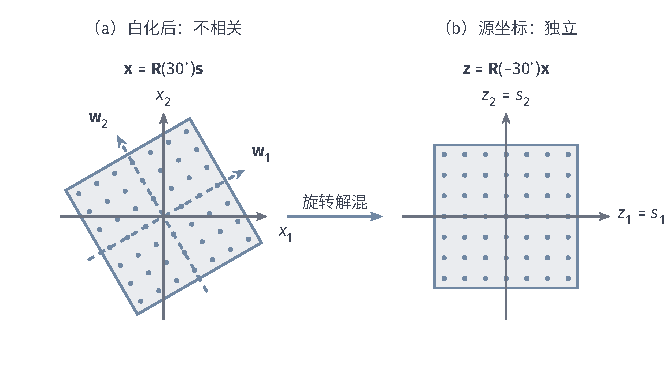
\includegraphics[width=112.000mm]{figures/04-classic-models/00-shared/tikz/dim-ica-whitening/figure.pdf}
  \caption{白化与独立源恢复的区别。设$s_1,s_2$独立且均服从$\mathcal{U}[-\sqrt3,\sqrt3]$，$\bm{R}(\theta)$为逆时针旋转矩阵。左图为$\bm{x}=\bm{R}(30^\circ)\bm{s}$，右图为逆旋转恢复的$\bm{s}$；两者协方差均为$\bm{I}_2$，只有右侧所示坐标对应独立源。实线轮廓为总体支持域，圆点为确定性格点，虚线箭头为解混方向。图为无量纲构造示意，未运行ICA优化；该方形解混本身不减少维数。}
  \label{fig:dim-ica-whitening}
\end{figure}

FastICA用光滑非二次函数$G$构造非高斯性对比量。单位方向$\bm{u}$在白化数据上产生方差为$1$的投影$\bm{u}^{\top}\widetilde{\bm{x}}$，可以将其与标准高斯变量$\nu$比较：
\begin{equation}
  J_G(\bm{u})
  =\left[
    \mathbb{E}G(\bm{u}^{\top}\widetilde{\bm{x}})
    -\mathbb{E}G(\nu)
  \right]^2,
  \qquad \lVert\bm{u}\rVert_2=1.
  \label{eq:dim-fastica-contrast}
\end{equation}
该目标近似前述负熵，其性质取决于$G$的选择。令$g=G'$；括号内的差非零、且期望与微分可交换时，$J_G$的球面驻点满足$\mathbb{E}G(\bm{u}^{\top}\widetilde{\bm{x}})$的约束驻点方程
\[
  \bm{a}(\bm{u})
  :=\mathbb{E}\!\left[\widetilde{\bm{x}}
       g(\bm{u}^{\top}\widetilde{\bm{x}})\right]
  =\beta\bm{u},
  \qquad
  \beta=\bm{u}^{\top}\bm{a}(\bm{u}).
\]
乘子$\beta$对应单位范数约束。近似求解时，在当前点固定$\beta$，并将Jacobian中的
$\mathbb{E}[\widetilde{\bm{x}}\widetilde{\bm{x}}^{\top}
g'(\bm{u}^{\top}\widetilde{\bm{x}})]$
近似为$c\bm{I}$，其中$c=\mathbb{E}g'(\bm{u}^{\top}\widetilde{\bm{x}})$。白化给出单位协方差，加上$g'$权重后的矩阵仍需这一步近似。若$c-\beta\ne0$，近似Newton步为
\[
  \bm{u}-\frac{\bm{a}(\bm{u})-\beta\bm{u}}{c-\beta}
  =\frac{c\bm{u}-\bm{a}(\bm{u})}{c-\beta}.
\]
方向可作符号翻转，归一化又消去非零标量，所以更新可直接使用$\bm{a}(\bm{u})-c\bm{u}$。将期望换成样本平均，从当前单位方向$\bm{u}^{(t)}$出发，就得到FastICA固定点更新：
\begin{equation}
  \begin{aligned}
  \bm{v}^{(t+1)}
    &=\frac1n\sum_{i=1}^{n}
      \widetilde{\bm{x}}_i
           g((\bm{u}^{(t)})^{\top}\widetilde{\bm{x}}_i)\\
    &\quad-\left[\frac1n\sum_{i=1}^{n}
      g'((\bm{u}^{(t)})^{\top}\widetilde{\bm{x}}_i)\right]\bm{u}^{(t)},\\
  \bm{u}^{(t+1)}
    &=\bm{v}^{(t+1)}/\lVert\bm{v}^{(t+1)}\rVert_2.
  \end{aligned}
  \label{eq:dim-fastica}
\end{equation}
常用$G(u)=\log\cosh u$或$G(u)=u^4/4$，对应$g(u)=\tanh u$和$g(u)=u^3$；后者的四次矩对极端值更敏感。多个成分可逐个与已求方向正交化，也可整组对称正交化。停止时检查方向变化，并把符号翻转计为同一方向\scite{hyvarinen1999fastica}

FastICA的收敛速度取决于源分布、对比函数与初始化，更新向量接近零时需重新初始化或调整设置。Infomax按输出非线性最大化输出熵，采用梯度更新；JADE通过联合对角化四阶累积量矩阵使用高阶统计信息。比较这些算法的成本，需要同时计入每次更新所用的信息与运算。

\subsubsection{小结}
\label{sec:dim-ica-summary}

ICA从去相关转向独立源识别，依赖源独立、非高斯与可识别性条件。标准方形ICA仍输出原维数；先截断白化空间，或取源数少于通道数的模型，才同时压缩。源数多于通道数时是欠定混合，通常需要稀疏等额外结构；非线性混合、相关源、多个高斯源及强噪声也需要不同的识别条件与算法。

\subsection{非负矩阵分解（NMF）}
\label{sec:dim-nmf}

词频、光谱强度与像素亮度为非负量，可以尝试将观测解释成多个成分的相加。\term{非负矩阵分解}（nonnegative matrix factorization, NMF）要求基与系数都非负，使每个成分增加重构值，而不通过正负抵消参与表示。

% 为两条完整的历史文献边注保留空间。
\Needspace{12\baselineskip}
非负结构可以与不同的误差模型配合。Paatero与Tapper在1994年根据环境测量误差加权残差，并在正矩阵分解中施加非负约束\scite{paatero1994nmf}Lee与Seung在1999年用人脸和文本说明加性表示如何形成组成成分\scite{lee1999nmf}两项工作分别强调测量约束与部件表示，损失及应用假设也随所解释的对象而变。

\subsubsection{模型结构}
\label{sec:dim-nmf-structure}

将非负观测排成$\bm{X}\in\mathbb{R}_{+}^{n\times d}$，寻找较少的共享基及各样本的非负系数：
\begin{equation}
  \bm{X}\approx\bm{W}\bm{H},\qquad
  \bm{W}\in\mathbb{R}_{+}^{n\times k},\quad
  \bm{H}\in\mathbb{R}_{+}^{k\times d}.
  \label{eq:dim-nmf-factorization}
\end{equation}
此处$\bm{W}$存放样本系数，与PCA的正交基约定不同；第$i$行是样本$i$的表示，$\bm{H}$各行是共享基。文档可由主题词模式相加，光谱可由成分谱相加。非负约束规定这种加性关系，基是否局部化、系数是否稀疏以及主题是否可读，则需要数据与额外约束支持。

图\ref{fig:dim-nmf-parts}用固定的横条与竖条基演示加性重构。九个像素按行展开后，$\bm{H}$的两行为基的转置，系数$(0.6,1.0)$给出右侧图案。中心像素同时获得两项贡献，值为$1.6$。这一固定字典下，两系数足以描述该图案；压缩成本还需计入字典，一般观测也可能存在重构误差。

\begin{figure}[htbp]
  \centering
  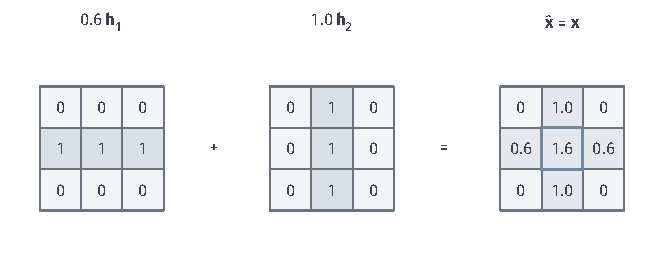
\includegraphics[width=112.000mm]{figures/04-classic-models/00-shared/tikz/dim-nmf-parts/figure.pdf}
  \caption{两个非负基的加性重构。左侧两幅$3\times3$栅格分别给出未加权的横条、竖条基，外侧系数为$0.6$与$1.0$；右侧为逐像素加权和，粗框中心格等于$0.6+1.0=1.6$。数值无量纲，本构造恰好精确重构，不表示NMF总能学出这样的部件或保证唯一分解。}
  \label{fig:dim-nmf-parts}
\end{figure}

观测类型决定怎样衡量重构误差。连续观测常用$\frac12\lVert\bm{X}-\bm{W}\bm{H}\rVert_F^2$，对应固定方差高斯残差的似然；非负计数可以使用广义KL散度，也称I散度：
\begin{equation}
  \mathcal{L}_{\mathrm{KL}}
  =\sum_{i,j}\left[
      \bm{X}_{i,j}\log\frac{\bm{X}_{i,j}}{(\bm{W}\bm{H})_{i,j}}
      -\bm{X}_{i,j}+(\bm{W}\bm{H})_{i,j}\right].
  \label{eq:dim-nmf-kl}
\end{equation}
计算采用$0\log(0/u)=0$；观测$\bm{X}_{i,j}>0$而重构为零时，损失为无穷大。条件独立Poisson计数的负对数似然与上式只差数据常数；存在过度离散时，则需要调整观测模型。

NMF的分解具有尺度和排列自由度。对正对角矩阵$\bm{D}$，$\bm{W}\bm{H}=(\bm{W}\bm{D})(\bm{D}^{-1}\bm{H})$，同时交换基与对应系数也保持重构。稀疏、平滑和归一化可以减少部分歧义，唯一性仍需相应识别条件。

\subsubsection{参数学习}
\label{sec:dim-nmf-learning}

基与系数的联合优化非凸，固定一侧后，平方误差子问题则是非负约束凸问题。Lee与Seung的乘法更新用非负比率维持可行性；下面的乘除均逐元素计算，两侧按顺序更新\scite{lee2001nmf}
\begin{equation}
  \begin{aligned}
    \bm{W}&\leftarrow\bm{W}\odot
       \frac{\bm{X}\bm{H}^{\top}}
        {\bm{W}\bm{H}\bm{H}^{\top}},\\
    \bm{H}&\leftarrow\bm{H}\odot
       \frac{\bm{W}^{\top}\bm{X}}
        {\bm{W}^{\top}\bm{W}\bm{H}}.
  \end{aligned}
  \label{eq:dim-nmf-mu}
\end{equation}
正初始化且更新有定义时，辅助函数可以证明目标不增加；结合非负下界，目标值序列便收敛。参数是否到达驻点或极小值还需进一步条件。零元素可能被锁定，因此实现还要处理零分母、检查约束梯度残差，并比较多次初始化结果。

其他求解方式可以更直接地检查约束残差。投影梯度用$\max(0,\cdot)$返回非负区域，交替非负最小二乘更充分地求各子问题；HALS和坐标下降逐个更新基或系数，可以利用稀疏结构。达到给定精度的速度取决于损失、稀疏性和初始化，目标单调性只说明下降性质\scite{lin2007nmf}

固定$\bm{H}$后，新样本通过非负最小二乘或相应KL目标编码。平方误差下求$\min_{\bm{w}\geq0}\lVert\bm{x}-\bm{H}^{\top}\bm{w}\rVert_2^2$，需要求系数，而非复用一个线性投影。稠密平方误差更新的主要乘法约需$O(ndk)$，训练总成本还取决于迭代次数。

\subsubsection{小结}
\label{sec:dim-nmf-summary}

NMF以加性成分解释非负数据，求解和使用需要考虑非凸目标及表示歧义。低秩PCA与NMF一般都存在重构误差，压缩是否足够精确要由所保留成分决定。中心化后的负值若通过平移变成非负，也会改变加性分解的含义，需要由任务支持这一预处理。

在相应归一化与计数似然约定下，式\eqref{eq:dim-nmf-kl}的NMF与概率隐语义索引具有同一目标，更新算法则不同\scite{ding2008nmf-plsi}潜在狄利克雷分配还为文档主题比例设置先验\scite{blei2003}更多约束可分别用于多轴数据、基的构成、成分关系、稀疏结构和层次组织，对应非负张量分解、凸NMF、正交NMF、稀疏NMF及深度NMF。采用哪些约束，应依据实际成分需要具有什么含义。

\subsection{稀疏编码与字典学习}
\label{sec:dim-sparse-coding}

一个图像块可能仅包含几条边缘，却要从许多位置和方向选择它们。可以准备较大的基向量库，让每个样本只激活少数基。\term{稀疏编码}（sparse coding）在固定字典中求这些活跃系数，\term{字典学习}（dictionary learning）进一步从数据学习共享的基。

Olshausen与Field在1996年研究自然图像的统计规律是否能解释初级视觉皮层响应的局部性、方向选择性与空间频率选择性。他们用稀疏线性编码学习具有这些性质的基，并与小波表示比较\scite{olshausen1996}这给视觉神经科学和信号表示建立了联系；感受野外观相似的证据，仍不足以确定生物学习过程与该算法相同。

\subsubsection{模型结构}
\label{sec:dim-sparse-coding-structure}

把共享基作为$\bm{D}\in\mathbb{R}^{d\times p}$的列，称$\bm{d}_j$为字典原子，$p$为原子数。允许$p>d$时，字典称为过完备。样本由$\bm{x}_i\approx\bm{D}\bm{\alpha}_i$重构，$\bm{\alpha}_i\in\mathbb{R}^{p}$只激活少数坐标。取$\lambda>0$控制稀疏惩罚的强度，通过误差与惩罚的加权和选择字典和系数：
\begin{equation}
  \begin{aligned}
  \min_{\bm{D},\{\bm{\alpha}_i\}}\quad&
   \sum_{i=1}^{n}\left[
      \tfrac12\lVert\bm{x}_i-\bm{D}\bm{\alpha}_i\rVert_2^2
      +\lambda\lVert\bm{\alpha}_i\rVert_1\right],\\
  \text{约束}\quad&\lVert\bm{d}_j\rVert_2\leq1
                 \quad(j=1,\ldots,p).
  \end{aligned}
  \label{eq:dim-dictionary-objective}
\end{equation}
若字典无限放大、系数相应缩小，重构不变而$\ell_1$惩罚降低；列范数约束排除了这种尺度退化。此模型允许正负系数和非正交基，表示长度甚至可以超过原维数，与NMF的非负及PCA的正交约束不同。

只使用一个含$s$个原子的支持集时，重构落在至多$s$维的线性子空间；更换活跃原子，就切换到其他子空间。稀疏表示因而可以用多个子空间组织不同样本，而非要求它们都位于同一光滑低维流形。活跃集合随输入改变，编码通常也是非线性的。

\subsubsection{参数学习}
\label{sec:dim-sparse-coding-learning}

给定字典后，每个样本独立求Lasso型系数，可用坐标下降、LARS或近端梯度。对一个样本，取$L\geq\lVert\bm{D}^{\top}\bm{D}\rVert_2$且$L>0$，ISTA把重构误差的梯度步与稀疏惩罚结合：
\begin{equation}
  \bm{\alpha}^{(t+1)}
  =\mathcal{S}_{\lambda/L}\left(
      \bm{\alpha}^{(t)}
      +L^{-1}\bm{D}^{\top}
          (\bm{x}-\bm{D}\bm{\alpha}^{(t)})\right).
  \label{eq:dim-ista}
\end{equation}
该更新先沿重构误差的负梯度移动，再作$\ell_1$惩罚的软阈值近端映射。FISTA增加外推，在固定字典的凸子问题条件下改善目标值收敛率；字典与系数联合学习仍需单独分析\scite{beck2009fista}

给定编码，记$\bm{A}=[\bm{\alpha}_1,\ldots,\bm{\alpha}_n]\in\mathbb{R}^{p\times n}$，字典步最小化$\frac12\lVert\bm{X}^{\top}-\bm{D}\bm{A}\rVert_F^2$并满足列范数约束。MOD用无约束解$\bm{X}^{\top}\bm{A}^{\dagger}$更新方向，常见实现再归一化各列。各字典列共同影响重构残差，无约束解后逐列归一化一般不能得到列范数约束下的精确解。需要严格下降时，应采用适当的约束求解或验证更新。

K-SVD通常采用$\lVert\bm{\alpha}_i\rVert_0\leq s$的活跃原子数约束。更新一个原子时，先去掉其他原子的重构，只保留使用该原子的样本，再用残差的秩一SVD同时更新原子与活跃系数。该求解配合的是非零项数约束，与式\eqref{eq:dim-dictionary-objective}的$\ell_1$目标不同\scite{aharon2006ksvd}

在线字典学习按小批样本更新，积累编码二阶统计量及观测交叉统计量以近似求字典，减少反复扫描全数据的开销。总成本还取决于原子数、每个稀疏子问题的精度和更新次数，一次遍历不能确定达到指定精度的完整成本\scite{mairal2009online}

\subsubsection{小结}
\label{sec:dim-sparse-coding-summary}

少量活跃原子可以组合出多种信号，适合去噪、修复和可组合模式的表示。新样本仍需求系数，因此使用时需要优化预算。压缩感知进一步研究从少量线性测量恢复稀疏信号，恢复条件还涉及测量矩阵的受限等距等性质。

字典和活跃约束可以随任务扩展：判别式字典利用标签，结构稀疏规定原子共同出现的方式，卷积稀疏编码在位置间共享滤波器。稀疏自编码器和层次表示也使用类似约束，算法与理论是否相通仍需比较目标和更新。本章讨论稀疏编码，是因为它以少数线性成分描述样本，而非因为编码向量一定更短。

\subsection{随机投影（Random Projection）}
\label{sec:dim-rp}

前述投影和字典都先从数据学习。流式数据维数很高时，也可以问：预先固定一个映射，是否仍能近似保留点间欧氏距离？\term{随机投影}（random projection）按指定分布抽取矩阵，再统一变换全部样本。Johnson--Lindenstrauss引理给出这种构造的保距依据，保证针对抽取映射前固定的有限点集，以较高概率同时成立\scite{johnson1984jl}

实现这种映射还要考虑生成和计算成本。Achlioptas于2003年构造离散随机矩阵，让投影由属性的加减、聚合和统一缩放实现\scite{achlioptas2003}其变化在于算术操作，有限点集上的几何保证仍不依赖先拟合数据。

\subsubsection{模型结构}
\label{sec:dim-rp-structure}

用$\bm{\Pi}\in\mathbb{R}^{k\times d}$编码$\bm{z}=\bm{\Pi}\bm{x}$。独立高斯元素$\bm{\Pi}_{i,j}\sim\mathcal{N}(0,1/k)$给出最直接的构造：对固定$\bm{x}$，平方范数的平均值为
\[
  \mathbb{E}_{\bm{\Pi}}\lVert\bm{\Pi}\bm{x}\rVert_2^2
  =\lVert\bm{x}\rVert_2^2.
\]
该期望只说明平均保范数。一次采样要同时服务整批样本，还需控制偏离均值的尾概率，再让各点对的误差同时受限。

稀疏矩阵进一步减少乘法和存储。Achlioptas的元素以$1/6$概率取$\sqrt{3/k}$、以$1/6$概率取$-\sqrt{3/k}$，其余取零，也可建立集中界。Li、Hastie与Church研究更稀疏的构造时，还需考虑输入分量的集中程度；二阶矩相同并不足以支持任意稀疏率下的同一误差界\scite{li2006sparserp}

快速Johnson--Lindenstrauss变换用随机符号、Hadamard变换及后续抽样或稀疏映射组织计算。结构化变换部分约为$O(d\log d)$，总成本还包括输出维数和精度相关项。与直接存储$kd$个高斯元素相比，它对内存、算术和输入尺寸有不同要求\scite{ailon2009fjlt}

\subsubsection{参数学习}
\label{sec:dim-rp-learning}

随机投影直接生成映射，需要选择的是$k$、矩阵分布和稀疏程度。训练与新样本使用相同矩阵，稠密编码每样本约需$O(kd)$次运算。分布式环境若用共同种子复现映射，还要固定伪随机数实现和矩阵元素的生成顺序。

输出维数决定误差、点数和失败概率之间的取舍。下面的充分条件往往保守，给出的$k$若已超过$d$，就没有实际压缩收益。可以在训练或验证数据上测量距离失真，比较较小维数，或先随机压缩到中等维数再做PCA、最近邻搜索；下游结果则按任务另行评价。

对映射抽取前固定的有限点集，高斯随机投影给出同时保留平方距离的充分维数条件，可用来设置候选$k$（参见\BookTheoremRef{thm:probability-johnson-lindenstrauss}{第一卷“数学准备”的“高斯随机投影的距离保持”定理}）。观察映射后，从这批固定点中选择要比较的点对，仍被同时保距事件覆盖；观察映射后再构造点集之外的新查询，则超出这里的固定点集保证。

\subsubsection{理论分析}
\label{sec:dim-rp-theory}

\paragraph{表达能力}
随机投影用线性映射近似保留指定点集的距离，输出维数限定能保留的信息。它没有从样本学习非线性流形，有限点集的保距也没有为完整分布建立可逆表示。

要用一次采样同时服务全部点对，需要让维数足以控制整批失败概率。给定点数、相对误差和失败概率后，可使用以下充分条件。

对$n\geq2$个预先固定的点，取$0<\varepsilon,\delta<1$。
上述定理给出充分条件
\[
  k\geq\frac{8}{\varepsilon^2}\log\frac{n(n-1)}{\delta},
\]
使同一高斯投影以至少$1-\delta$的概率同时把全部点对的平方距离保持在原值的
$1\pm\varepsilon$倍内。这里$\delta$控制整批点对的失败概率，不是每一对单独的失败概率。

在相应参数区间，JL的$\varepsilon^{-2}\log n$维数尺度有匹配下界\scite{larsen2017jl}例如要求失败概率至多$1/n$时，可取$k\geq24\log n/\varepsilon^2$。具体集中界决定常数；主要尺度随点数对数增长，上界本身不直接依赖$d$。

\paragraph{收敛性}
映射按预设分布采样，所以没有训练目标的迭代求解。稠密高斯矩阵生成和存储为$O(kd)$规模，每个输入也约需$O(kd)$运算。增大$k$是在保距精度和计算成本之间选择，而非提高训练收敛速度。

\paragraph{泛化性}

保距结论只覆盖预先固定的有限点集。$k<d$时，非零核空间中的向量被压成零，因此无法同时保留$\mathbb{R}^{d}$内所有距离。独立于映射预先指定的新查询可以加入点集重新计算联合界；观察映射后在固定点集之外构造的新查询则需额外分析。

\subsubsection{小结}
\label{sec:dim-rp-summary}

随机投影可以立即用于流式或超高维预处理，所保留的是给定度量下的有限点集几何。预测相关特征和能否压到二维，需要另外检验。局部敏感哈希、压缩感知和随机化线性代数分别关注碰撞概率、稀疏集合保距和子空间逼近；随机Fourier特征与特征哈希也使用随机映射，但各自近似的对象不同。

\subsection{核主成分分析（Kernel PCA）}
\label{sec:dim-kpca}

线性投影难以保留弯曲变化时，可以先通过非线性特征重新描述输入。\term{核主成分分析}（kernel principal component analysis, Kernel PCA）在这种特征空间中选择主方向，用核函数计算内积，省去显式列出特征的步骤。Schölkopf、Smola与Müller于1998年提出这一核特征值方法\scite{dimScholkopf1998}

\subsubsection{模型结构}

这里需要的特征由第\ref{sec:classic-overview-kernel-validity}节的正定核$K$定义，记Hilbert空间为$\mathcal{H}$、映射为$\bm{\phi}$。训练核矩阵及中心化矩阵$\bm{H}$沿用第\ref{sec:classic-overview-kernel-matrix}节。核PCA以保留特征方差为目标，核SVM的间隔目标则用于分类。

方差要相对于训练特征均值计算，因此取
\[
  \bar{\bm{\phi}}=\frac1n\sum_i\bm{\phi}(\bm{x}_i),
  \qquad
  \bm{\phi}_{\mathrm{c}}(\bm{x})=\bm{\phi}(\bm{x})-\bar{\bm{\phi}}.
\]
方向$\bm{v}\in\mathcal{H}$上的经验协方差运算为
\begin{equation}
  \label{eq:dim-kpca-covariance}
  \widehat{\mathcal{C}}\bm{v}
  =\frac1n\sum_i
    \bm{\phi}_{\mathrm{c}}(\bm{x}_i)
    \langle\bm{\phi}_{\mathrm{c}}(\bm{x}_i),\bm{v}\rangle_{\mathcal{H}}.
\end{equation}
若$\widehat{\mathcal{C}}\bm{v}=\lambda^{\mathrm{C}}\bm{v}$且$\lambda^{\mathrm{C}}>0$，右侧的有限和说明$\bm{v}$落在中心化训练特征张成的空间。正特征值方向因而可以用训练特征展开；零特征值方向没有这一约束。

将方向写为$\bm{v}_\ell=\sum_i(\bm{\alpha}_\ell)_i\bm{\phi}_{\mathrm{c}}(\bm{x}_i)$，并令$\bm{K}_{\mathrm{c}}=\bm{H}\bm{K}\bm{H}$。代入协方差方程，核矩阵特征值满足$\lambda_\ell^{\mathrm{K}}=n\lambda_\ell^{\mathrm{C}}$，把特征空间的谱计算转成样本矩阵计算。

\subsubsection{参数学习}

核矩阵的单位特征向量需要缩放，才能成为特征空间单位方向的展开系数。令$\bm{u}_\ell$为中心化核矩阵的欧氏单位特征向量，归一化关系为
\begin{equation}
  \label{eq:dim-kpca-normalization}
  \begin{aligned}
    \bm{K}_{\mathrm{c}}\bm{u}_\ell
      &=\lambda_\ell^{\mathrm{K}}\bm{u}_\ell,
      \qquad\lVert\bm{u}_\ell\rVert_2=1,\\
    \bm{\alpha}_\ell
      &=\frac{\bm{u}_\ell}{\sqrt{\lambda_\ell^{\mathrm{K}}}},\\
    \lVert\bm{v}_\ell\rVert_{\mathcal{H}}^2
      &=\bm{\alpha}_\ell^{\top}\bm{K}_{\mathrm{c}}\bm{\alpha}_\ell=1.
  \end{aligned}
\end{equation}
将各训练点投到方向$\bm{v}_\ell$，得到表示矩阵的一列：
\begin{equation}
  \label{eq:dim-kpca-training}
  \bm{Z}_{:,\ell}
  =\bm{K}_{\mathrm{c}}\bm{\alpha}_\ell
  =\sqrt{\lambda_\ell^{\mathrm{K}}}\,\bm{u}_\ell
  =\lambda_\ell^{\mathrm{K}}\bm{\alpha}_\ell.
\end{equation}
$\bm{u}_\ell$在欧氏范数下归一化，$\bm{\alpha}_\ell$则使特征空间方向范数为一。因此训练坐标是$\sqrt{\lambda_\ell^{\mathrm{K}}}\bm{u}_\ell$，展开系数乘上的尺度要按上式计算，不能改为$\sqrt{\lambda_\ell^{\mathrm{K}}}\bm{\alpha}_\ell$。

选择核相当于先决定观察输入的哪些变化。图\ref{fig:dim-kernel-radial}用$\phi(\bm{x})=\lVert\bm{x}\rVert_2^2$只记录半径平方，$K(\bm{x},\bm{y})=\phi(\bm{x})\phi(\bm{y})$由此为正半定核。两圆样本数相同，均值为$(1+4)/2=2.5$，中心化坐标为$-1.5$和$1.5$。径向差异得以保留，角度在特征映射中已丢失，后续PCA无法恢复。

\begin{figure*}[htbp]
  \centering
  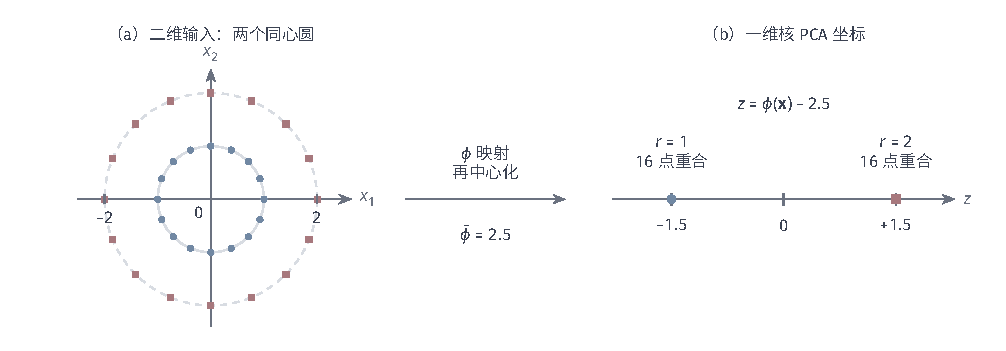
\includegraphics[width=169.000mm]{figures/04-classic-models/00-shared/tikz/dim-kernel-radial/figure.pdf}
  \caption{由核选择保留量的构造例子。左图在半径为$1,2$的圆上各取16个等角度样本，圆点与方点区分两圈。所示特制核对应标量特征$\phi(\bm{x})=\lVert\bm{x}\rVert_2^2$，中心化核矩阵秩为1；选择图示主轴方向，核PCA坐标为$\pm1.5$。右侧每个标记表示16点重合，坐标无量纲。此结果依赖所选核，不能推广为任意高斯核或多项式核的输出。}
  \label{fig:dim-kernel-radial}
\end{figure*}

新样本必须沿用训练特征均值，才能与训练表示处于同一坐标系。令$\bm{k}(\bm{x})_i=K(\bm{x}_i,\bm{x})$，中心化及投影为
\begin{equation}
  \label{eq:dim-kpca-extension}
  \begin{aligned}
    \bm{k}_{\mathrm{c}}(\bm{x})
      ={}&\bm{k}(\bm{x})-\frac1n\bm{K}\bm{1}\\
         &-\frac1n\bm{1}\bm{1}^{\top}\bm{k}(\bm{x})
          +\frac1{n^2}\bm{1}\bm{1}^{\top}\bm{K}\bm{1},\\
    z_\ell(\bm{x})
      ={}&\bm{\alpha}_\ell^{\top}\bm{k}_{\mathrm{c}}(\bm{x}).
  \end{aligned}
\end{equation}
两个减项分别扣除与训练均值的内积，末项补回均值自内积。只减新核向量自身均值会漏掉这些量；加入新点重算均值，则是在改变原先的映射。

常用核的全矩阵构造约需$O(n^2d)$，存储为$O(n^2)$，稠密谱分解为$O(n^3)$。Nystr\"om近似使用代表列减少矩阵计算，随机Fourier特征则对合适的平移不变核构造有限特征后再做线性PCA。近似误差需要单独评价，适用核也各有条件。

高斯核带宽过大时，各核值接近，中心化信号变弱；带宽过小时，核矩阵接近单位阵，主方向难以辨认。距离中位数可作初始尺度，再用任务验证选择。监督任务中的中心化和主方向均应在训练折拟合。

\subsubsection{理论分析}
\label{sec:dim-kpca-theory}

\paragraph{表达能力}
核PCA在核特征空间中选择线性主方向，相对于原输入的非线性由特征映射提供。核、训练中心与保留维数共同限定表示；其高方差方向对下游任务是否有用，需要相应评价。

\paragraph{收敛性}

固定正定核后，经验方差目标可由谱分解全局求解，核矩阵近似及求谱精度决定数值误差。相同谱计算还连接点间距离：第\ref{sec:dim-mds}节定义经典MDS后，定理\ref{thm:dim-kpca-mds}将证明核诱导距离与中心化核PCA给出相同训练坐标。该联系针对特征距离，局部重构和图平滑则使用不同目标。

\paragraph{泛化性}

固定有界核、可分特征空间并独立同分布采样时，经验协方差算子随样本量增加逼近总体对象。目标谱与其余谱之间有正间隔，主子空间也可稳定逼近\scite{blanchard2007kpca}数据自适应核或趋零谱隙会改变分析所需条件。

样本外公式定义了新点的编码，并未评价分布外的质量；新点与训练点核值几乎相同时，表示可能缺少区分。若要重构原输入，还需另求截断特征的原像，有些特征甚至没有对应输入。

\subsubsection{小结}

核PCA先用核规定特征几何，再保留主要变化方向。谱求解与样本外公式使表示可复用，所得结果则依赖核合法性、训练中心化、带宽和谱隙。原空间几何的恢复还需要额外条件。

\subsection{模型对比与总结}
\label{sec:dim-linear-comparison}

矩阵形式相似的方法，保留的信息和编码成本可以不同。表\ref{tab:dim-linear-comparison}同时列出训练目标与新样本机制，分别回答怎样选表示、怎样复用表示。方形ICA保持维数，过完备稀疏编码甚至增加坐标数；它们在此共同使用线性投影或线性组合，但压缩方式各异。

\begin{table*}[htbp]
  \centering
  \small
  \begin{tabularx}{\linewidth}{@{}l>{\RaggedRight\arraybackslash}X>{\RaggedRight\arraybackslash}X>{\RaggedRight\arraybackslash}X@{}}
    \toprule
    方法 & 主要目标与约束 & 新样本的表示 & 典型边界\\
    \midrule
    PCA & 正交投影下保留方差 & 中心化后矩阵乘法 & 对尺度、异常值敏感\\
    CCA & 配对视图的相关性最大 & 两侧分别线性投影 & 需配对观测，易过拟合相关性\\
    ICA & 独立源的线性解混 & 白化及解混乘法 & 独立性、非高斯性与可识别性\\
    NMF & 非负基与非负系数重构 & 非负约束推断 & 非凸、通常不唯一\\
    稀疏编码 & 少量原子重构观测 & 稀疏优化 & 可为高维编码，需控制推断成本\\
    随机投影 & 随机矩阵近似保距 & 固定矩阵乘法 & 维数、误差与失败概率的权衡\\
    核PCA & 特征空间方差 & 训练中心化核投影 & 核几何、样本展开与原空间重构\\
    \bottomrule
  \end{tabularx}
  \caption{线性投影与线性组合方法的比较。目标成立均依赖各小节的具体条件；“新样本可编码”不等于编码具有统计泛化保证。}
  \label{tab:dim-linear-comparison}
\end{table*}

求解方式进一步决定预算：PCA与CCA作谱分解，ICA优化非高斯对比量，NMF与字典学习交替更新，随机投影生成固定矩阵。迭代方法还需计入稀疏结构、停止精度与总轮数。基可以追溯原始特征，是否对应可解释概念仍要由数据和任务验证。

响应或类别已知时，可以直接寻找与预测有关的方向。第\ref{sec:regression-regularization}节的PCR按输入方差选成分，PLS让响应参与构造；第\ref{sec:classification-lda-reduction}节的线性判别分析比较类间和类内散度。切片逆回归利用$\mathbb{E}[\bm{x}\mid y]$的变化，在相应线性及非退化条件下恢复有效方向，对条件均值无法显示的对称响应则可能遗漏\scite{li1991sir}这些目标把任务信息加入方向选择，改变了单纯保留输入方差的准则。

监督降维组合特征形成新方向，特征选择保留原坐标子集，两者可以共同使用。比较预测收益时，应将响应参与的方向学习、特征选择和预测器都放在训练折内，以相同下游风险比较无监督表示、监督表示和不降维基线。

选择线性组合时，需要先确定保留的是方差、视图相关、独立源、非负成分、稀疏支持还是点对距离。第\ref{sec:dim-probabilistic}节的因子分析会加入特征特异噪声；下一节MDS则从距离恢复坐标，并在欧氏输入下联系PCA。弯曲结构若无法由原空间线性基充分描述，还需要不同的特征或非线性关系。

\section{基于距离的降维}
\label{sec:dim-distance}

对象之间的差异有时比原始坐标更容易取得，例如相似性评分或编辑距离。此时需要根据差异安排位置，而非直接投影特征。多维缩放提供了这种坐标恢复；下一节还会把差异限制到局部邻域，用来研究弯曲几何。

\subsection{多维缩放（MDS）}
\label{sec:dim-mds}

感知评分给出对象间差异，却没有给出对象坐标。\term{多维缩放}（multidimensional scaling, MDS）寻找低维位置，使坐标关系尽量符合这些差异。Young与Householder于1938年研究距离对坐标的代数约束，为坐标恢复建立了几何依据\scite{dimYoung1938}

Torgerson在1952年系统提出经典MDS时，还要处理心理距离怎样测量。刺激比较的差异可能缺少确定零点，因此原工作先估计比较距离中的未知加性常数，再分析维数和刺激坐标\scite{dimTorgerson1952}差异输入本身也有测量假设，这里的加性常数与下面的坐标、核矩阵中心化承担不同作用。

\subsubsection{模型结构}

将对象差异记为对称矩阵$\bm{D}\in\mathbb{R}^{n\times n}$，要求$\bm{D}_{i,j}\geq0$、$\bm{D}_{i,i}=0$。它可以来自欧氏、编辑、图距离或人工评分；这些关系未必能在指定维数中由欧氏距离实现。MDS的拟合准则决定采用哪一种近似。

要恢复欧氏几何，可以先从距离平方求中心化内积。\term{经典MDS}（classical MDS）采用这一转换，令$\bm{1}\in\mathbb{R}^n$为全一向量、$\bm{I}_n$为单位矩阵：
\begin{equation}
  \label{eq:dim-mds-centering}
  \begin{aligned}
    \bm{H}&=\bm{I}_n-\frac{1}{n}\bm{1}\bm{1}^{\top},\\
    \bm{D}^{\circ2}_{i,j}&=(\bm{D}_{i,j})^2,\\
    \bm{B}&=-\frac12\bm{H}\bm{D}^{\circ2}\bm{H}.
  \end{aligned}
\end{equation}
$\circ2$是逐元素平方。左右乘$\bm{H}$分别扣去列、行均值，即双中心化；欧氏输入得到的$\bm{B}$是中心化坐标的Gram矩阵，记录两两内积且为半正定。

从$\bm{B}$的正谱取得实数坐标。记$\lambda_1\geq\cdots\geq\lambda_r>0$，相应欧氏单位特征向量为$\bm{u}_1,\ldots,\bm{u}_r$；选择$k\leq r$后，坐标为
\begin{equation}
  \label{eq:dim-mds-coordinates}
  \bm{Z}=\bm{U}_k\bm{\Lambda}_k^{1/2},
  \qquad
  \bm{Z}_{i,\ell}=\sqrt{\lambda_\ell}\,(\bm{u}_\ell)_i.
\end{equation}
$\bm{U}_k$收集所选特征向量，$\bm{\Lambda}_k$收集相应特征值。其平方根缩放使坐标内积逼近$\bm{B}$，最小化的内积残差称为strain：
\begin{equation}
  \label{eq:dim-mds-strain}
  \min_{\substack{\bm{Z}\in\mathbb{R}^{n\times k}\\
                  \bm{Z}^{\top}\bm{1}=\bm{0}}}
  \left\lVert\bm{B}-\bm{Z}\bm{Z}^{\top}\right\rVert_{\mathrm{F}}^2.
\end{equation}
非欧氏差异可能使$\bm{B}$含负特征值。半正定秩约束近似舍弃负谱，保留最大的至多$k$个正特征值；这种内积近似通常也会改变输入距离。

任务若直接比较距离数值，可以让\term{度量MDS}（metric MDS）最小化距离残差。给定对称非负权重$w_{i,j}$，记$\delta_{i,j}(\bm{Z})=\lVert\bm{z}_i-\bm{z}_j\rVert_2$，常用应力（stress）目标为
\begin{equation}
  \label{eq:dim-mds-stress}
  S(\bm{Z})
  =\sum_{i<j}w_{i,j}
    \bigl(\delta_{i,j}(\bm{Z})-\bm{D}_{i,j}\bigr)^2.
\end{equation}
strain比较内积，stress比较距离。虽然距离与中心化内积可互相转换，两种残差平方和仍有不同的最优近似。有些文献也将经典MDS称为metric scaling，本章按实际目标区分。

当差异顺序比数值更可信时，\term{非度量MDS}（nonmetric MDS）用非递减函数$g(\bm{D}_{i,j})$作为式\eqref{eq:dim-mds-stress}中的目标距离，同时估计$g$和$\bm{Z}$。尺度约束排除共同缩到零的退化，保序要求作用于拟合差异；有限维坐标仍可能无法满足所有严格次序。Kruskal于1964年将顺序信息与应力准则结合\scite{dimKruskal1964}

\subsubsection{参数学习}

经典MDS的平方Frobenius目标可以沿正交特征方向分解。半正定约束排除负谱，秩约束保留较大的正谱，因此双中心化和谱截断给出全局最优表达；特征向量仍需数值求解。

距离残差通常采用迭代拟合，也可以按距离选择权重。例如所有非对角距离$\bm{D}_{i,j}>0$时，\term{Sammon映射}使用
\begin{equation}
  \label{eq:dim-sammon}
  S_{\mathrm{Sammon}}(\bm{Z})
  =\frac{1}{\sum_{i<j}\bm{D}_{i,j}}
    \sum_{i<j}
    \frac{\bigl(\delta_{i,j}(\bm{Z})-\bm{D}_{i,j}\bigr)^2}
         {\bm{D}_{i,j}}.
\end{equation}
小距离的相同绝对误差在此受到更大惩罚，使局部距离更受重视。它仍是近似目标，零差异需要合并对象或另定权重\scite{dimSammon1969}

应力型MDS可用梯度法、拟牛顿法，或\term{SMACOF}（scaling by majorizing a complicated function）。SMACOF在当前坐标构造与目标相切的二次上界，再最小化该上界；记上界为$Q$，下降关系为
\[
  S(\bm{Z}^{(s+1)})
  \leq Q(\bm{Z}^{(s+1)}\mid\bm{Z}^{(s)})
  \leq Q(\bm{Z}^{(s)}\mid\bm{Z}^{(s)})
  =S(\bm{Z}^{(s)}).
\]
非度量MDS可以交替求保序回归和坐标更新。目标非负且不增加时，目标值收敛；迭代点是否到达驻点、极小或全局最优仍要另查。实践中可以用经典MDS初始化并比较多次运行，SMACOF的构造与实现见de Leeuw和Mair的系统介绍\scite{dimDeLeeuw2009}

完整稠密经典MDS需要$O(n^2)$存储，谱分解通常为$O(n^3)$。部分谱或Nystr\"om近似可以减少计算；标志点MDS先嵌入代表点，再按到代表点的距离扩展，近似质量依赖代表点的覆盖。

\subsubsection{理论分析}
\label{sec:dim-mds-theory}

\paragraph{表达能力}
MDS以低维点间几何拟合距离或相异度。指定维数中的欧氏关系有结构限制，任意相异度未必满足，因此谱截断和应力拟合都可能留下无法消除的失真。

\paragraph{收敛性}

经典MDS的全局最优针对内积目标；应力型MDS的迭代通常在适当条件下保证下降。要进一步联系PCA，需要让两者处理同一批欧氏观测，并比较同一中心化坐标的谱截断。

设$\bm{D}$来自坐标矩阵$\bm{X}$各行的欧氏距离，中心化坐标为$\bm{X}_{\mathrm{c}}=\bm{H}\bm{X}$。平移不改变这些距离，双中心化得到
\[
  \bm{B}=\bm{H}\bm{X}\bm{X}^{\top}\bm{H}
  =\bm{X}_{\mathrm{c}}\bm{X}_{\mathrm{c}}^{\top}.
\]
该Gram矩阵来自中心化后的$\bm{X}_{\mathrm{c}}$。选择相同维数和相应奇异方向时，PCA与经典MDS共享谱截断；证明的关键是展开距离平方，说明双中心化怎样消去平移项并恢复该Gram矩阵。

\begin{theorem}[欧氏距离下经典MDS与PCA的关系]
  \label{thm:dim-mds-pca}
  设$\bm{X}^{\top}\bm{1}=\bm{0}$，$\bm{D}_{i,j}=\lVert\bm{x}_i-\bm{x}_j\rVert_2$，且$1\leq k\leq\operatorname{rank}(\bm{X})$。若PCA与经典MDS选取相互对应的前$k$个奇异方向，则两者的坐标都可取为$\bm{U}_k\bm{\Sigma}_k$，从而得到相同的坐标Gram矩阵$\bm{U}_k\bm{\Sigma}_k^2\bm{U}_k^{\top}$。同一所选子空间内的坐标可相差右侧正交变换，而Gram矩阵保持不变。
\end{theorem}
\begin{proof}
  令$\bm{a}\in\mathbb{R}^n$满足$a_i=\lVert\bm{x}_i\rVert_2^2$。展开距离平方并双中心化，得到
  \[
    \begin{aligned}
      \bm{D}^{\circ2}
        &=\bm{a}\bm{1}^{\top}+\bm{1}\bm{a}^{\top}
          -2\bm{X}\bm{X}^{\top},\\
      \bm{B}
        &=\bm{H}\bm{X}\bm{X}^{\top}\bm{H}
         =\bm{X}\bm{X}^{\top}.
    \end{aligned}
  \]
  第一、第二项消失，是因为$\bm{H}\bm{1}=\bm{0}$；末步使用样本已经中心化。对薄奇异值分解$\bm{X}=\bm{U}\bm{\Sigma}\bm{V}^{\top}$，有$\bm{B}=\bm{U}\bm{\Sigma}^2\bm{U}^{\top}$。MDS坐标与PCA得分因而分别为
  \[
    \bm{Z}_{\mathrm{MDS}}=\bm{U}_k\bm{\Sigma}_k,
    \qquad
    \bm{X}\bm{V}_k=\bm{U}_k\bm{\Sigma}_k.
  \]
  在同一所选子空间内旋转坐标轴不改变Gram矩阵。
\end{proof}

等价对象是同一保留维数$k$下的中心化坐标Gram矩阵及其诱导距离，原特征轴并未恢复。只有$k=\operatorname{rank}(\bm{X}_{\mathrm{c}})$、保留全部正特征值时，坐标才保留全部输入欧氏距离；$k<\operatorname{rank}(\bm{X}_{\mathrm{c}})$时，两者共享一个改变原距离的谱截断。

截断若满足$\lambda_k=\lambda_{k+1}$，可以选择不同的最优部分子空间，结果未必只差一个$k$维旋转。小谱隙也使方向对距离扰动敏感；评价稳定性时可比较对齐坐标、子空间或重构距离。

核特征距离也具有同一内积展开，因而第\ref{sec:dim-kpca}节预告的联系可以按相同方式证明。

\begin{theorem}[核诱导距离下的等价关系]
  \label{thm:dim-kpca-mds}
  设$K$为正定核，记$\bm{K}_{i,j}=K(\bm{x}_i,\bm{x}_j)$。训练点间的特征距离为
  \[
    \bm{D}_{i,j}^2
    =\bm{K}_{i,i}+\bm{K}_{j,j}-2\bm{K}_{i,j}.
  \]
  对此距离进行经典MDS，与对$\bm{K}$进行中心化核PCA，在选择相同正特征子空间和归一化后给出相同训练坐标。重特征值和截断处的非唯一性与定理\ref{thm:dim-mds-pca}相同。
\end{theorem}
\begin{proof}
  令向量$\bm{a}$的元素$a_i=\bm{K}_{i,i}$，距离平方矩阵为$\bm{a}\bm{1}^{\top}+\bm{1}\bm{a}^{\top}-2\bm{K}$。双中心化消去前两项，得到$\bm{B}=\bm{H}\bm{K}\bm{H}=\bm{K}_{\mathrm{c}}$。式\eqref{eq:dim-mds-coordinates}与式\eqref{eq:dim-kpca-training}因而输出相同的$\bm{U}_k\bm{\Lambda}_k^{1/2}$。
\end{proof}

\paragraph{泛化性}

新样本上的使用需要分开看统计估计和坐标扩展。距离来自独立同分布欧氏观测时，MDS与PCA的等价关系可以接入协方差估计分析；任意差异矩阵则要另给差异的生成机制和估计误差。

新对象到训练对象的距离已知时，可以固定原坐标作经典MDS扩展。记这些距离平方为$s_i$，$\bar s=n^{-1}\sum_i s_i$；训练距离的行均值为$r_i=n^{-1}\sum_j\bm{D}_{i,j}^2$，总均值为$\bar r=n^{-1}\sum_i r_i$。相对训练中心的内积与坐标为
\begin{equation}
  \label{eq:dim-mds-extension}
  \begin{aligned}
    b_i&=-\frac12(s_i-\bar s-r_i+\bar r),\\
    \bm{z}(\bm{x})
      &=\bm{\Lambda}_k^{-1/2}\bm{U}_k^{\top}\bm{b}.
  \end{aligned}
\end{equation}
第一行沿用训练中心计算内积，第二行用最小二乘取得相应坐标。训练点保持固定，与加入新点重做MDS的结果不同；非欧氏差异下，该扩展是相对已有表示的近似投影\scite{dimBengio2003}

\subsubsection{小结}

MDS根据差异安排坐标，经典、度量与非度量形式分别拟合内积、距离与顺序。相同欧氏观测和相同保留维数下，经典MDS与中心化PCA共享谱截断；降到数据秩以下，两者都会改变原距离。距离的可嵌入性、截断维数与矩阵规模共同限定结果。

\subsection{模型对比与总结}

已有特征且关心方差，可以直接用PCA学习投影；只有对象差异时，可以用MDS安排位置。选择MDS的形式，要确认输入表达的是内积几何、距离数值还是可信顺序，再用相应目标和样本外机制评价。不同目标的数值没有直接可比性。

\section{基于邻域的降维}
\label{sec:dim-neighbors}
\label{sec:dim-manifold}

如果原空间距离主要在小范围内可信，可以先建立邻域，再组织全局坐标。第\ref{sec:classic-overview-neighborhood}节给出了邻域与图的共同机制；这里按要保留的关系展开：图路径描述长度，局部组合描述重构，图上平滑和随机游走描述连通性，邻居概率或边权则用于安排可观察的布局。

几何方法中的部分模型假设数据接近\term{流形}（manifold），即局部可以用少量连续坐标描述的空间。弯曲结构的方向随位置改变，直接投影可能混合沿曲面相距较远的点；局部自由度少，整体却仍可能无法在同维数中无失真展开。各方法需要的采样和几何条件将在具体构造中给出。

以下继续使用$n,d,k,m,q$与$\bm{X},\bm{Z}$。布局的输入距离记为$\delta_{i,j}=\lVert\bm{x}_i-\bm{x}_j\rVert_2$，低维距离记为$r_{i,j}=\lVert\bm{z}_i-\bm{z}_j\rVert_2$。训练坐标是这些方法直接求得的对象，接收新样本还需规定相应映射或扩展。

\subsection{等距映射（Isomap）}
\label{sec:dim-isomap}

弯曲流形上，穿过观测空间的直线距离与沿流形的最短长度可以相差很大。后者为\term{测地距离}（geodesic distance），记为$d_{\mathcal{M}}$。\term{等距映射}（isometric mapping, Isomap）用邻域图最短路径估计它，再由经典MDS恢复坐标。Tenenbaum、de Silva与Langford于2000年提出该方法；同年的LLE则选择局部重构关系作为保留对象\scite{dimTenenbaum2000}

\subsubsection{模型结构}

将样本作为顶点建立无向图$\mathcal{G}=(V,E)$，连接距离不超过$\varepsilon$的点，或对称化$q$近邻。近邻并集与互近邻给出的边不同，需要明确采用哪一种。每条边的长度为$\ell_{i,j}=\lVert\bm{x}_i-\bm{x}_j\rVert_2$，是路径成本；长度越小越近，与后文连接越强数值越大的相似度权重不同。

路径只能沿图中边行走。将一条路径的边长相加，再在全部可行路径中选择最短者：
\begin{equation}
  \label{eq:dim-isomap-distance}
  d_{\mathcal{G}}(i,j)
  =\min_{\substack{i=i_0,\ldots,i_s=j\\(i_{a-1},i_a)\in E}}
    \sum_{a=1}^{s}\ell_{i_{a-1},i_a}.
\end{equation}
由全部图距离组成$\bm{D}_{\mathcal{G}}$，计算$\bm{B}_{\mathcal{G}}=-\tfrac12\bm{H}\bm{D}_{\mathcal{G}}^{\circ2}\bm{H}$，再按式\eqref{eq:dim-mds-coordinates}取坐标。局部连接、全局路径和欧氏表示依次承担三项工作；路径近似与MDS拟合也分别引入误差。

邻域决定路径能否合理近似曲面长度。图\ref{fig:dim-geodesic}中的两段曲线在观测空间接近，沿曲线却相距很远；跨过弯曲部分的一条错误边，可能缩短许多点对的图距离。
\begin{figure}[htbp]
  \centering
  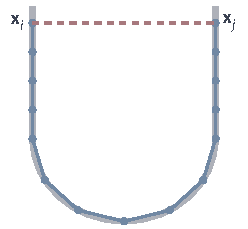
\includegraphics[width=42.012mm]{figures/04-classic-models/00-shared/tikz/dim-geodesic/figure.pdf}
  \caption{一维弯曲曲线上的距离示意。曲线表示嵌入观测空间的一维流形，曲线上的点表示离散样本；沿相邻样本连接的折线表示邻域图路径，其各段长度之和用于近似沿曲线的测地距离。顶部红色虚线是两点间的欧氏直线；若邻域取值过大而把它误纳入图中，就会形成穿过流形外部、低估测地距离的短路。图为几何示意，不是算法输出或实验结果，未给出数值误差。}
  \label{fig:dim-geodesic}
\end{figure}

\subsubsection{参数学习}

暴力建邻域约需$O(n^2d)$时间，空间索引的收益依赖维数与分布。非负边长下，从每点运行二叉堆Dijkstra的成本为$O(n(|E|+n)\log n)$，Floyd--Warshall为$O(n^3)$。后续稠密MDS仍需$O(n^2)$存储、通常$O(n^3)$的完整谱分解；稀疏邻域并未使全体点对距离也稀疏。

输入度量、预处理、$q$或$\varepsilon$以及$k$共同决定结果。小邻域可能断连，大邻域可能跨过卷层，噪声和非均匀采样也会改变可用尺度。可检查连通分量、边长分布及随邻域变化的稳定性。距离相关残差$1-R^2$提供辅助诊断，但对统一缩放不敏感，仍需直接检查失真与测地近似。

标志点Isomap（Landmark Isomap）选$s\ll n$个代表点，从这些点出发求最短路径，保留$s\times n$距离表，再用标志点MDS和距离扩展安排其余点。de Silva与Tenenbaum的原文还讨论共形变换下的距离修正\scite{dimDeSilva2002}标志点减少计算规模，共形修正改变几何假设，是两项不同的选择。

\subsubsection{理论分析}
\label{sec:dim-isomap-theory}

\paragraph{表达能力}
Isomap的表示由两层近似组成：邻域最短路径拟合测地距离，低维欧氏坐标拟合图距离。错误捷径或无法等距展开的流形，会使同时保留全部距离的目标难以实现。

\paragraph{收敛性}
固定图后，最短路径算法求出图距离，经典MDS求相应的谱近似。数值精度可以通过路径与谱求解检查，邻域是否近似真实几何则属于建模条件；计算完成并未消除两层近似的误差。

\paragraph{泛化性}
样本增加时，希望图距离也越来越接近测地距离。覆盖不足会漏掉必要连接，边长失真过大又会形成捷径，下面的确定性界分别控制这两种问题。

覆盖空隙$h$衡量流形上各位置到最近样本的最大测地距离，单边失真$\eta$衡量弦长比测地距离短多少。证明沿最短测地线放置分割点，再用附近样本替代它们，构造图路径以控制误差；这里尚未要求该距离能嵌入指定$k$维。

\begin{theorem}[覆盖条件下的图距离界]
  \label{thm:dim-isomap-bound}
  设$\mathcal{M}\subset\mathbb{R}^d$连通，任意两点间存在最短测地线。样本的测地填充距离为
  \[
    h=\sup_{\bm{x}\in\mathcal{M}}\min_i
      d_{\mathcal{M}}(\bm{x},\bm{x}_i).
  \]
  图连接全部欧氏距离不超过$\varepsilon$的样本对，并以欧氏弦长为边长。假设$h<\varepsilon/2$，且存在$0\leq\eta<1$，使每条边都满足
  \[
    \lVert\bm{x}_i-\bm{x}_j\rVert_2
    \geq(1-\eta)d_{\mathcal{M}}(\bm{x}_i,\bm{x}_j).
  \]
  则对所有样本对，图距离有限，且
  \begin{equation}
    \label{eq:dim-isomap-bound}
    \begin{aligned}
      d_{\mathcal{G}}(i,j)
        &\geq(1-\eta)d_{\mathcal{M}}(\bm{x}_i,\bm{x}_j),\\
      d_{\mathcal{G}}(i,j)
        &\leq\left(1+\frac{2h}{\varepsilon-2h}\right)
          d_{\mathcal{M}}(\bm{x}_i,\bm{x}_j).
    \end{aligned}
  \end{equation}
\end{theorem}
\begin{proof}
  对任意图路径，各边弦长至少是对应测地距离的$1-\eta$倍。将其相加，再用测地距离的三角不等式，就得到下界。

  为证明上界，记两端点的测地距离为$L$，取连接它们的一条最短测地线，令$a=\varepsilon-2h>0$。若$L=0$，结论成立；否则沿测地线每隔$a$放一个分割点，末段不足$a$，总段数为$s=\lceil L/a\rceil$。保留原来的两个样本端点，把每个内部分割点替换成测地距离不超过$h$的样本。相邻替代样本的测地距离至多$a+2h=\varepsilon$，欧氏距离不更大，因此构成图中的边；重复样本可略去。

  每个内部分割点的替代误差至多在两条相邻边中各计一次，而两端点无需替代，故所构造路径的长度至多
  \[
    L+2h(s-1)
    \leq L+\frac{2hL}{\varepsilon-2h}.
  \]
  图最短路径不长于这条路径，得到上界，同时证明图中这些端点相连。
\end{proof}

对一列样本与邻域，若$h/\varepsilon\to0$且$\eta\to0$，两侧界给出样本点对上的统一相对距离一致性。曲率有界仍需配合足够小的邻域尺度，才能排除卷层间连接。若采样独立且密度有正下界，可以研究覆盖空隙$h$的概率界，条件还需包括体积、内在维数、覆盖数和密度。

图距离准确之后，还要判断是否存在欧氏坐标保留它。单位球面赤道上四个等间隔点，相邻测地距离为$\pi/2$，两组对点为$\pi$。若都能成为欧氏距离，三角不等式取等号迫使另外两点成为同一对点的中点；它们却应相距$\pi$，产生矛盾。这说明真实测地距离本身也可能无法同时欧氏实现。

当流形与$\mathbb{R}^m$中凸区域在长度意义下等距时，区域内测地长度就是直线距离，这是恢复平直坐标的一类充分情形。带孔非凸区域即使局部平直，绕孔长度仍可能不同。后续MDS还需控制距离误差对内积和谱子空间的影响。新点可通过到邻居的边长加训练图距离，再用式\eqref{eq:dim-mds-extension}定位；原图固定，不等于加入点后重新计算全体最短路径。

\subsubsection{小结}

Isomap将局部边长汇总成全局长度，适合考察可展开的几何结构。覆盖、无短路邻域与目标欧氏维数共同决定可靠性。断连分量之间没有有限路径，需分别处理或依据额外信息连接；随意填入大数会引入新的距离假设。

\subsection{局部线性嵌入（LLE）}
\label{sec:dim-lle}

局部邻域还能提供另一种约束：一个点由哪些邻居、按什么权重重构。\term{局部线性嵌入}（locally linear embedding, LLE）将样本写成邻居的仿射组合，再要求低维坐标保持这些组合关系。它用距离选邻居、用局部内积求权重，但不计算全体点对的路径距离。

LLE与Isomap在2000年同一期《Science》上相邻发表，都利用局部信息建立全局坐标。LLE原文致谢中记载了作者与Tenenbaum的讨论，以及对方提供Isomap代码的帮助\scite{dimRoweis2000}两项工作有实际交流，采用的约束却不同：Isomap拟合路径长度，LLE拟合局部重构关系。

\subsubsection{模型结构}

令$\mathcal{N}_i$包含样本$i$的$q$个邻居。重构矩阵$\bm{W}\in\mathbb{R}^{n\times n}$只在邻居位置取非零权重，且每行权重和为一。通过最小化原空间的重构残差求这些权重：
\begin{equation}
  \label{eq:dim-lle-weights}
  \begin{aligned}
    \min_{\bm{W}}\quad&
      \sum_i\left\lVert\bm{x}_i-\sum_j\bm{W}_{i,j}\bm{x}_j
      \right\rVert_2^2,\\
    \text{满足}\quad&
      \bm{W}\bm{1}=\bm{1},\qquad
      \bm{W}_{i,j}=0\quad(j\notin\mathcal{N}_i).
  \end{aligned}
\end{equation}
行和为一使重构关系对整体平移不变：所有点加上同一个向量，中心点及其重构点同步移动。权重可以为负，因此组合是仿射的，未必是凸的。$\bm{W}$通常不对称，其元素也不能解释为随机游走概率。

固定$\bm{W}$后，在低维空间最小化同一组权重对应的残差。记$\bm{M}=(\bm{I}_n-\bm{W})^{\top}(\bm{I}_n-\bm{W})$，目标为
\begin{equation}
  \label{eq:dim-lle-embedding}
  \begin{aligned}
    \min_{\bm{Z}}\quad&
      \lVert(\bm{I}_n-\bm{W})\bm{Z}\rVert_{\mathrm{F}}^2
      =\operatorname{tr}(\bm{Z}^{\top}\bm{M}\bm{Z}),\\
    \text{满足}\quad&
      \bm{Z}^{\top}\bm{1}=\bm{0},\qquad
      \bm{Z}^{\top}\bm{Z}=n\bm{I}_k.
  \end{aligned}
\end{equation}
样本按行排列，因而残差写作$(\bm{I}_n-\bm{W})\bm{Z}$。中心化约束去掉整体平移，列正交与定范数约束防止坐标全部塌缩。这里选定的是代数尺度，未要求坐标距离等于原始距离。

图\ref{fig:dim-lle-weights}用权重$0.3,0.3,0.4$重构中心点。邻居移动后，以同一权重安排中心仍可得到零残差，三角形边长却已改变。完整LLE还需协调其他点的邻域并满足全局约束，图中只展示一项局部关系。

\begin{figure*}[htbp]
  \centering
  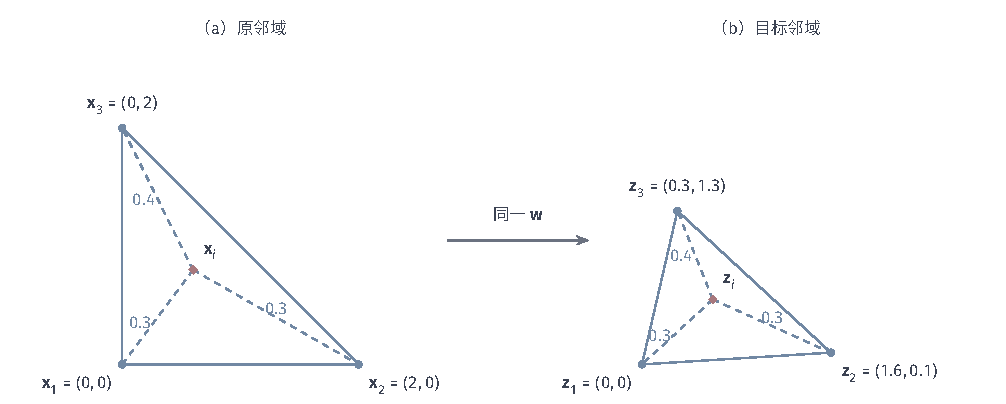
\includegraphics[width=169.000mm]{figures/04-classic-models/00-shared/tikz/dim-lle-weights/figure.pdf}
  \caption{LLE局部权重保持的示意。左图用二维局部坐标绘出三个邻居和菱形中心点；虚线旁为重构权重，其和为1。右图将邻居移至所标位置，同样的权重给出中心$(0.60,0.55)^\top$。两图使用相同的无量纲尺度，实线三角形的形状与边长可以改变。两个画面用于对照高维局部几何与目标邻域，不是完整LLE输出，也不表示一次二维到二维的降维。}
  \label{fig:dim-lle-weights}
\end{figure*}

\subsubsection{参数学习}

按固定顺序排列第$i$个邻域，令$\bm{A}_i\in\mathbb{R}^{q\times d}$的每行为$(\bm{x}_j-\bm{x}_i)^{\top}$，并记$\bm{C}_i=\bm{A}_i\bm{A}_i^{\top}$。该邻域的权重$\bm{w}_i\in\mathbb{R}^q$满足
\[
  \min_{\bm{1}^{\top}\bm{w}_i=1}
    \bm{w}_i^{\top}\bm{C}_i\bm{w}_i.
\]
当$\bm{C}_i$正定时，驻点条件为$\bm{C}_i\bm{w}_i=c\bm{1}$。用权重和为一确定$c$，得到
\begin{equation}
  \label{eq:dim-lle-local}
  \bm{w}_i
  =\frac{\bm{C}_i^{-1}\bm{1}}
         {\bm{1}^{\top}\bm{C}_i^{-1}\bm{1}}.
\end{equation}
求权重时直接解线性方程即可。$q>d$使$\bm{C}_i$必然奇异；即使$q\leq d$，局部样本接近低维切空间也可能造成秩亏或病态。可用$\bm{C}_i+\rho_i\bm{I}_q$改善条件数，例如令$\rho_i$与迹成比例。邻居全部重合时迹为零，需另设正的尺度下限或单独处理。加入正则项也改变了原重构目标。

行和约束给出$\bm{M}\bm{1}=\bm{0}$。在常数方向的正交补中，取最小的$k$个特征方向组成单位列矩阵$\bm{U}_k$，则$\bm{Z}=\sqrt n\,\bm{U}_k$解式\eqref{eq:dim-lle-embedding}。零空间只有常数方向时，才能取最小$k+1$个特征向量后丢掉一个。断连分量的指示向量也属于零空间；对于带符号权重，连通本身仍不足以保证零空间只有一维。

额外零模态会使部分坐标只给各分量分配常数，未表达分量内部的形状。分别嵌入各分量也无法由局部关系确定它们的相对位置、方向和尺度，断连问题仍需额外处理。

局部矩阵构造及求解约需$O(nq^2d+nq^3)$。全局阶段可依次乘$\bm{I}_n-\bm{W}$及其转置，无需显式形成$\bm{M}$；一次矩阵向量乘约为$O(nq)$。部分谱求解还受谱隙、迭代次数和重正交成本影响。邻居数$q$、输出维数$k$与正则尺度都需要选择。

局部重构关系为何可能在降维后保留，可以用坐标函数的Taylor展开解释。令邻居的局部位移为$\bm{\xi}_j$，对光滑函数$f$有
\[
  \begin{aligned}
    f(\bm{x}_i)-\sum_j\bm{W}_{i,j}f(\bm{x}_j)
    ={}&-\nabla f^{\top}\sum_j\bm{W}_{i,j}\bm{\xi}_j\\
       &+O\left(\sum_j|\bm{W}_{i,j}|
                  \lVert\bm{\xi}_j\rVert_2^2\right).
  \end{aligned}
\]
权重和为一消去常数项，加权位移接近零又使一阶项较小，剩余误差主要来自二阶变化。余项中出现权重绝对值，所以大幅正负抵消可能放大误差。噪声还会改变邻域和局部矩阵，局部近似是否可靠需要另行检查。

对新点先求局部重构权重，再以$\bm{z}(\bm{x})=\sum_{j\in\mathcal{N}(\bm{x})}w_j(\bm{x})\bm{z}_j$插值。训练坐标固定，这一步未重新求全局谱。邻域不稳定或新点远离训练支持时，插值可能失真。

\subsubsection{小结}

LLE以局部仿射关系连接各邻域，可靠性取决于邻域尺度、局部秩、权重稳定性和全局零空间。它省去全体点对最短路径，却未要求距离或角度精确保留。Hessian LLE增加局部二阶约束，局部切空间对齐（LTSA）估计并对齐切空间；本节比较将说明这些约束及其适用条件。

\subsection{拉普拉斯特征映射（Laplacian Eigenmaps）}
\label{sec:dim-le}

邻近点的坐标变化缓慢，也能成为降维约束。\term{拉普拉斯特征映射}（Laplacian Eigenmaps）将这种平滑性写成图上的二次能量，在防止塌缩的约束下求低能量坐标。Belkin与Niyogi在NIPS 2001介绍相关谱方法，2003年期刊论文展开其模型与几何联系\scite{dimBelkin2003}它与第\ref{sec:clustering-spectral}节的谱聚类共享建图、图拉普拉斯与低频特征方向；这里直接输出连续坐标，谱聚类再将谱表示转成簇分配。

\subsubsection{模型结构}

在对称邻域图上设非负权重$\bm{W}_{i,j}$。相邻点可取$\exp(-\lVert\bm{x}_i-\bm{x}_j\rVert_2^2/(4\tau))$或$1$，其他位置为零，$\tau>0$控制衰减尺度。令$b_i=\sum_j\bm{W}_{i,j}$、$\bm{D}_b=\operatorname{diag}(b_1,\ldots,b_n)$，图拉普拉斯为$\bm{L}=\bm{D}_b-\bm{W}$。对标量信号$\bm{f}\in\mathbb{R}^n$，由对称性有
\begin{equation}
  \label{eq:dim-le-energy}
  \bm{f}^{\top}\bm{L}\bm{f}
  =\frac12\sum_{i,j}\bm{W}_{i,j}(f_i-f_j)^2.
\end{equation}
能量非负，故$\bm{L}$半正定，常数信号的能量为零。将各坐标列的能量相加，得到
\begin{equation}
  \label{eq:dim-le-objective}
  \begin{aligned}
    \min_{\bm{Z}}\quad&
      \operatorname{tr}(\bm{Z}^{\top}\bm{L}\bm{Z}),\\
    \text{满足}\quad&
      \bm{Z}^{\top}\bm{D}_b\bm{Z}=\bm{I}_k,\qquad
      \bm{Z}^{\top}\bm{D}_b\bm{1}=\bm{0}.
  \end{aligned}
\end{equation}
度加权范数排除零解，加权中心化排除常数方向。缺少后一个约束，就可能将没有区分能力的常数列纳入嵌入。目标只惩罚邻近点的坐标差异，远点是否分开还由全局约束和所选模式决定。

\subsubsection{参数学习}

对坐标列求驻点，在常数的加权正交补中得到$\bm{L}\bm{v}=\lambda\bm{D}_b\bm{v}$。各点度为正时，令$\bm{u}=\bm{D}_b^{1/2}\bm{v}$，将它化成对称特征值问题：
\[
  \bm{L}_{\mathrm{sym}}\bm{u}=\lambda\bm{u},
  \qquad
  \bm{L}_{\mathrm{sym}}
  =\bm{I}_n-\bm{D}_b^{-1/2}\bm{W}\bm{D}_b^{-1/2}.
\]
求得单位向量后，要变回$\bm{v}=\bm{D}_b^{-1/2}\bm{u}$以满足模型的归一化。连通图的广义问题以常数为零特征向量，对称问题的零方向却与$\bm{D}_b^{1/2}\bm{1}$成比例。多个连通分量对应多个零模态，应一并识别；零度点也需单独处理，不能直接作逆度归一化。

若权重矩阵有$O(nq)$个非零元，一次矩阵向量乘为$O(nq)$。总求解成本还包括建图、$k$个方向的迭代及正交化。$q$控制哪些点连接，$\tau$控制连接强弱，$k$控制保留的模式数。过小带宽可能使部分度数接近零，过大带宽则削弱局部差异，可结合图诊断与任务表现选择。

\subsubsection{理论分析}
\label{sec:dim-le-theory}

\paragraph{表达能力}
表示由图上的低频模式组成，输出维数限定保留多少模式。它保留邻域平滑关系，但这些关系未必唯一确定全局几何；任务所需的快速变化也可能被截断。

\paragraph{收敛性}
固定非负邻域图后，广义特征值问题给出约束能量的全局最优解。截断处有谱隙时，所选子空间唯一。迭代速度取决于谱隙、预条件和残差要求；有限图上的数值收敛与采样图逼近流形属于不同问题。

\paragraph{泛化性}
讨论新样本时，需要将离散能量与连续几何联系起来。式\eqref{eq:dim-le-energy}对应的\term{Dirichlet能量}积分了函数沿流形的变化率平方。采用非负号约定$\Delta_{\mathcal{M}}=-\operatorname{div}_{\mathcal{M}}\nabla_{\mathcal{M}}$，在紧致无边界流形上有
\begin{equation}
  \label{eq:dim-dirichlet}
  \mathcal{E}(f)
  =\int_{\mathcal{M}}\lVert\nabla_{\mathcal{M}}f\rVert_2^2\,\mathrm{d}V
  =\int_{\mathcal{M}}f\Delta_{\mathcal{M}}f\,\mathrm{d}V.
\end{equation}
Laplace--Beltrami算子描述函数沿流形的局部变化，对应欧氏空间的负拉普拉斯。求均值为零、平方积分为一的最平滑函数时，给能量加入约束乘子，并沿光滑扰动$g$求导：
\[
  2\int_{\mathcal{M}}g\Delta_{\mathcal{M}}f\,\mathrm{d}V
  -2\lambda\int_{\mathcal{M}}gf\,\mathrm{d}V
  -2c\int_{\mathcal{M}}g\,\mathrm{d}V=0.
\]
分部积分产生第一项。取$g=1$得到$c=0$，再由扰动任意得到$\Delta_{\mathcal{M}}f=\lambda f$。逐次加入与已有特征函数正交的约束，就按频率从低到高得到函数方向。这一变分关系解释了低频坐标的平滑性。

图与流形之间要分别考察算子和谱。点态收敛作用于固定光滑函数，谱收敛则比较随样本改变的特征值与特征函数，前者不能直接推出后者。Belkin与Niyogi在2006年的谱收敛研究中，分别处理经验算子的谱逼近及小带宽下的连续谱逼近\scite{dimBelkin2006}

\begin{theorem}[一种定性的谱一致性结论]
  \label{thm:dim-le-spectral}
  设$\mathcal{M}$是紧致、连通、无边界的$C^\infty$嵌入$m$维黎曼流形，为简化常数令其体积为一。样本独立均匀采自$\mathcal{M}$。考虑全连接高斯图对应的经验算子
  \[
    \begin{aligned}
      \widehat{\mathcal{L}}_{n,\tau}f(\bm{x})
      ={}&\frac{1}{n\tau(4\pi\tau)^{m/2}}\\
      &\cdot\sum_{j=1}^n
        e^{-\lVert\bm{x}-\bm{x}_j\rVert_2^2/(4\tau)}
        \bigl(f(\bm{x})-f(\bm{x}_j)\bigr).
    \end{aligned}
  \]
  存在趋于零而足够缓慢的带宽序列$\tau_n$，使每个固定的低频特征值依概率收敛到$\Delta_{\mathcal{M}}$的相应特征值。将经验特征向量按该算子延拓并作$L^2(\mathcal{M})$归一化后，孤立单特征值对应的特征函数可在符号对齐后依概率收敛；重特征值应按相应有限维特征子空间比较。
\end{theorem}

该结论针对给定的全连接高斯算子，只断言存在合适带宽序列。归一化幂次用内在维数$m$，且算子未作度归一化。它与模型的广义特征值问题之间还需尺度校正：均匀采样下，度的极限趋向空间常数，可以联系两者；非均匀采样、稀疏截断或流形有边界时，要重新分析度、极限测度及边界条件。

非均匀密度$p$下，未修正的局部能量一般带$p^2$权重，密集区域因而更影响低频表示。谱收敛也未保证少量特征函数组成的映射单射或保留全部距离。新点可用核特征函数延拓，或另学映射。标签传播在给定类别语义下求得分，谱聚类输出簇，本节输出坐标；它们共享图平滑，但目标与评价不同（参见第\ref{sec:classification-label-propagation}、\ref{sec:clustering-spectral}节）。

\subsubsection{小结}

拉普拉斯特征映射从邻域权重中提取低频坐标，离散能量与Dirichlet能量的关系提供几何解释。求解时需正确处理特征向量归一化和全部零模态；解释采样极限时，还需区分点态收敛与谱收敛。坐标的含义由所建图决定，密度修正和全局距离保留都需要额外条件。

\subsection{扩散映射（Diffusion Map）}
\label{sec:dim-diffusion}

低频坐标的距离还能获得概率解释。\term{扩散映射}（diffusion map）比较从两个起点出发、经过相同步数后的到达分布：分布越相似，起点越接近。Coifman与Lafon在2006年将这一扩散距离写成谱坐标，并用时间参数选择表示尺度\scite{dimCoifman2006}

\subsubsection{模型结构}

以对称非负矩阵$\bm{K}$表示原始相似度，可用全连接高斯核或稀疏邻域权重。记原始度为$r_i$，密度重加权后的度为$b_i$，以避免与邻居数$q$混淆。归一化过程为
\begin{equation}
  \label{eq:dim-diffusion-normalization}
  \begin{aligned}
    r_i&=\sum_j\bm{K}_{i,j},&
    \widetilde{\bm{K}}_{i,j}
      &=\frac{\bm{K}_{i,j}}{r_i^\alpha r_j^\alpha},\\
    b_i&=\sum_j\widetilde{\bm{K}}_{i,j},&
    \bm{P}_{i,j}&=\frac{\widetilde{\bm{K}}_{i,j}}{b_i},
    \qquad 0\leq\alpha\leq1.
  \end{aligned}
\end{equation}
假设度数均为正。$\bm{P}$每行和为一，其元素表示一步转移概率。重加权后的度确定平稳分布：
\begin{equation}
  \label{eq:dim-diffusion-stationary}
  \pi_i=\frac{b_i}{\sum_j b_j},
  \qquad
  \pi_i\bm{P}_{i,j}=\pi_j\bm{P}_{j,i}.
\end{equation}
末式是细致平衡关系，故$\bm{\pi}^{\top}\bm{P}=\bm{\pi}^{\top}$。按行写分布与列向量方程$\bm P^\top\bm\pi=\bm\pi$等价（参见\BookSectionRef{sec:rv-markov}{第一卷“数学准备”的“历史条件下的状态依赖”小节}）。平稳分布使用$b_i$；只有$\alpha=0$等特殊情形，才可由原始$r_i$直接计算。

对整数$t\geq0$，以$p_t(i,j)=(\bm{P}^t)_{i,j}$表示$t$步转移概率。定义扩散距离
\begin{equation}
  \label{eq:dim-diffusion-distance}
  D_t^2(i,j)
  =\sum_{a=1}^n\frac{(p_t(i,a)-p_t(j,a))^2}{\pi_a}.
\end{equation}
距离比较整个到达分布，各目标点的差异按平稳概率校正；很少被访问的点上，同样的概率差会计入更大贡献。若两个起点有相同到达分布，距离也会为零，故一般可为伪度量。跨区域瓶颈减缓混合，使部分时间尺度仍能区分这些区域。

图\ref{fig:dim-diffusion-walk}中，两个团只由一条弱边相连。团内传播快，跨团传播慢，4步后大部分概率仍在起点一侧；64步时两行分布已更接近，仍未相同。扩散距离比较这些概率差，节点在示意图中的间隔不参与计算。

\begin{figure}[htbp]
  \centering
  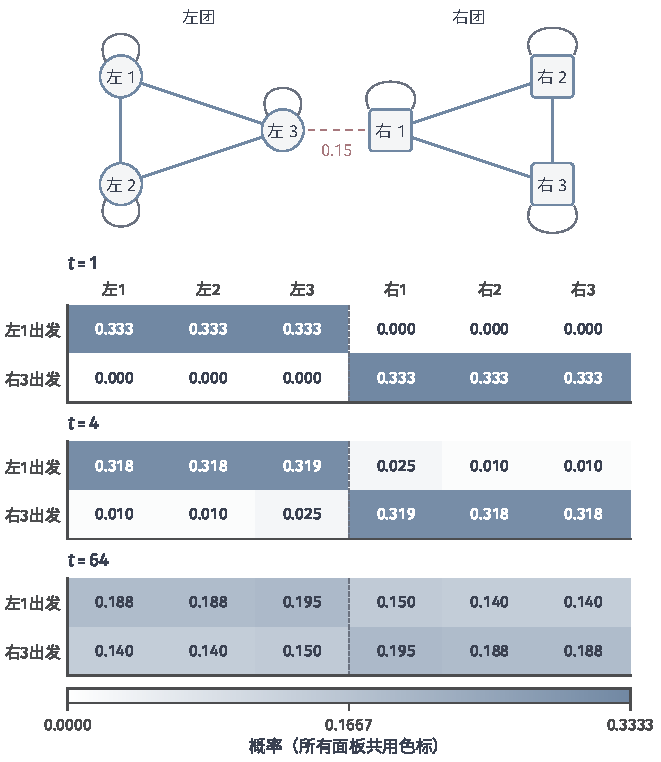
\includegraphics[width=105.412mm]{figures/04-classic-models/00-shared/matplotlib/dim-diffusion-walk/figure.pdf}
  \caption{扩散时间与跨团瓶颈。每团三个节点，团内边及所有自环权重为1，唯一跨团边权重为$0.15$。令$\alpha=0$并按行归一化，热图两行分别表示从左1、右3出发的$\bm{P}^t$对应行，六列为固定节点顺序；各时刻共用同一连续概率色标。数值由有理数矩阵乘法计算，显示三位小数，舍入后行和可能略偏离1。64步仍未充分混合；因图连通且有自环，极限分布均为$\bm{\pi}^{\top}=(20,20,21,21,20,20)/122$。}
  \label{fig:dim-diffusion-walk}
\end{figure}

\subsubsection{参数学习}

记$\bm{\Pi}=\operatorname{diag}(\pi_1,\ldots,\pi_n)$。由细致平衡，矩阵
\[
  \bm{S}=\bm{\Pi}^{1/2}\bm{P}\bm{\Pi}^{-1/2}
\]
为对称矩阵。取其欧氏单位特征向量$\bm{u}_\ell$，并令$\bm{\psi}_\ell=\bm{\Pi}^{-1/2}\bm{u}_\ell$，则
\begin{equation}
  \label{eq:dim-diffusion-eigenvectors}
  \begin{aligned}
    \bm{P}\bm{\psi}_\ell&=\lambda_\ell\bm{\psi}_\ell,\\
    \sum_i\pi_i\psi_\ell(i)\psi_r(i)&=\delta_{\ell,r}.
  \end{aligned}
\end{equation}
这些特征函数在$L^2(\bm{\pi})$内积下正交。连通图的常数特征对为$\lambda_0=1,\psi_0(i)=1$，其余特征值在$[-1,1]$内。再满足非周期性时，非平凡特征值的绝对值小于一。连通图保留正自环即可保证非周期性，无自环二部图却可能出现$-1$特征值。

非负对称权重仍可能有负特征值，应按$|\lambda_1|\geq|\lambda_2|\geq\cdots$选择扩散模态。全连接半正定核经对角缩放仍半正定，此时才可按非负特征值降序选取；稀疏截断可能破坏半正定性。$k$维扩散坐标定义为
\begin{equation}
  \label{eq:dim-diffusion-map}
  \bm{\Psi}_{t,k}(i)
  =\bigl(\lambda_1^t\psi_1(i),\ldots,
         \lambda_k^t\psi_k(i)\bigr)^{\top}.
\end{equation}
将这些坐标按行放置，得到$n\times k$矩阵。$t$对应转移矩阵的整数幂；含负特征值时，直接令$t$取任意实数将失去这一解释。

稠密矩阵的构造、存储及完整谱分解成本与核PCA同阶。稀疏权重降低矩阵向量乘成本，总求谱时间仍受$k$、谱间隔及精度影响。除邻域或带宽与$k$外，还要选择$\alpha$和$t$；同一组谱可在不同$t$下重新加权，无需重复分解。

\subsubsection{理论分析}
\label{sec:dim-diffusion-theory}

\paragraph{表达能力}
扩散时间选择几何尺度，输出维数决定保留多少转移模态。坐标拟合的是给定核及归一化对应的扩散距离；原空间的其他距离可能改变。

谱表示在有限图上就成立。先求其精确关系与截断界，再讨论采样极限，可以分别判断代数近似与几何近似。

全部非平凡模态精确表示扩散距离，未保留的谱及平稳概率共同控制截断误差。下面在$L^2(\bm{\pi})$中展开转移概率，用正交性消去交叉项；核尺度与有限图的结构误差仍需另行检查。

\begin{theorem}[扩散距离的谱表示与截断界]
  \label{thm:dim-diffusion-isometry}
  设$\bm{P}$由连通的对称非负权重构造，$\pi_i>0$，特征函数按式\eqref{eq:dim-diffusion-eigenvectors}归一化。对整数$t\geq0$，全部非平凡模态给出
  \begin{equation}
    \label{eq:dim-diffusion-identity}
    D_t^2(i,j)
    =\sum_{\ell=1}^{n-1}\lambda_\ell^{2t}
      \bigl(\psi_\ell(i)-\psi_\ell(j)\bigr)^2.
  \end{equation}
  当$t=0$时按$\bm{P}^0=\bm{I}_n$约定所有模态系数为一。若按特征值绝对值排序，$k<n-1$且$i\ne j$，截断的平方距离误差$R_{t,k}$满足
  \begin{equation}
    \label{eq:dim-diffusion-tail}
    \begin{aligned}
      R_{t,k}(i,j)
        &:=D_t^2(i,j)
          -\lVert\bm{\Psi}_{t,k}(i)-\bm{\Psi}_{t,k}(j)\rVert_2^2,\\
      0\leq R_{t,k}(i,j)
        &\leq|\lambda_{k+1}|^{2t}
          \left(\frac1{\pi_i}+\frac1{\pi_j}\right).
    \end{aligned}
  \end{equation}
\end{theorem}
\begin{proof}
  对称矩阵$\bm{S}$的谱分解给出
  \[
    p_t(i,a)=\pi_a\sum_{\ell=0}^{n-1}
      \lambda_\ell^t\psi_\ell(i)\psi_\ell(a).
  \]
  令$c_\ell=\lambda_\ell^t(\psi_\ell(i)-\psi_\ell(j))$，则$c_0=0$。代入定义，展开平方并使用加权正交性：
  \[
    \begin{aligned}
      D_t^2(i,j)
        &=\sum_a\pi_a
          \left(\sum_{\ell=1}^{n-1}c_\ell\psi_\ell(a)\right)^2\\
        &=\sum_{\ell,r=1}^{n-1}c_\ell c_r
          \sum_a\pi_a\psi_\ell(a)\psi_r(a)
         =\sum_{\ell=1}^{n-1}c_\ell^2.
    \end{aligned}
  \]
  其中$\pi_a$来自分子中$\pi_a^2$除以定义中的$\pi_a$，不能再次消去。截断后余项是$\ell>k$的非负和。由绝对值排序及完整正交基关系，
  \[
    \begin{aligned}
      R_{t,k}
        &\leq|\lambda_{k+1}|^{2t}
          \sum_{\ell=1}^{n-1}
            (\psi_\ell(i)-\psi_\ell(j))^2,\\
      \sum_{\ell=0}^{n-1}\psi_\ell(i)\psi_\ell(j)
        &=\frac{\delta_{i,j}}{\sqrt{\pi_i\pi_j}},
    \end{aligned}
  \]
  对$i\ne j$展开平方，即得所述上界；$i=j$时两种距离和余项都为零。
\end{proof}

保留全部$n-1$个模态时距离精确，截取$k$维则一般有误差。式\eqref{eq:dim-diffusion-tail}同时含谱尾部与平稳概率，稀少区域可能有更大的绝对误差界。增大时间虽使该界缩小，真实扩散距离也随之缩小，不能据此保证相对精度改善。

不可约且非周期的有限链满足$|\lambda_\ell|<1$，故$t\to\infty$时，各起点的到达分布趋于$\bm{\pi}^{\top}$，距离也趋于零。混合前的较大$t$突出慢模态，过大的$t$则丢失区分。连续时间可另用$\exp[-s(\bm{I}_n-\bm{P})]$，以$e^{-s(1-\lambda_\ell)}$加权。

使用同一组对称权重时，拉普拉斯广义问题与转移矩阵满足
\[
  (\bm{D}_b-\bm{W})\bm{v}=\mu\bm{D}_b\bm{v}
  \quad\Longleftrightarrow\quad
  \bm{P}\bm{v}=(1-\mu)\bm{v}.
\]
两者因而共享特征方向。将选定模态的时间权重设为一，并调整归一化，可得到无时间加权的拉普拉斯坐标；$L^2(\bm{\pi})$与$\bm{D}_b$的归一化还差全局尺度。负谱存在时，按绝对值排序的扩散映射可能选中拉普拉斯高端模态，这一选择也需计入比较。

\paragraph{收敛性}
固定满足细致平衡的转移矩阵后，扩散坐标由谱分解求得。残差决定数值精度，谱分离和求解器影响迭代速度。游走时间$t$选择表示尺度，与求谱算法的迭代次数分别控制不同问题。

\paragraph{泛化性}

密度修正要在采样极限中解释。在光滑正密度$p$、足够采样及小高斯带宽的内点极限下，生成元含有与$2(1-\alpha)\nabla_{\mathcal{M}}\log p$有关的漂移。$\alpha=1$消去主导密度漂移，使极限扩散由流形几何决定；有限样本仍可能有密度影响。$\alpha=0$保留密度作用，适用于任务本身关注该概率结构的情形。

新点可用Nystr\"om方式延拓。沿用训练核及$r_j$，计算$r(\bm{x})=\sum_j\kappa(\bm{x},\bm{x}_j)$，按训练归一化构造$p(\bm{x},j)$。当$\lambda_\ell\ne0$时，有
\begin{equation}
  \label{eq:dim-diffusion-extension}
  \psi_\ell(\bm{x})
  =\frac1{\lambda_\ell}\sum_jp(\bm{x},j)\psi_\ell(j),
  \qquad
  z_\ell(\bm{x})=\lambda_\ell^t\psi_\ell(\bm{x}).
\end{equation}
该式固定训练度和谱，将特征方程延伸到新点。小特征值的倒数会放大误差，零特征值需其他处理。错误连接对传播的影响取决于它如何改变瓶颈，使用多条路径也不能保证减弱每一条错误边的作用。

\subsubsection{小结}

扩散映射将谱坐标的距离解释为到达分布的差异。重加权度确定平稳分布，特征函数在$L^2(\bm{\pi})$中归一化，时间因子控制模态强弱。$\alpha$重加权调整密度作用；扩散小波则用扩散算子的幂组织多尺度函数基\scite{dimCoifmanMaggioni2006}

向量扩散映射将局部方向的对齐也纳入传播，可研究切向量的一致性，因而还需估计局部坐标系。这些扩展共享多步传播，但仍受核尺度、采样误差、慢模态选择、混合时间与延拓稳定性限制。

\subsection{随机邻居嵌入（SNE）}
\label{sec:dim-sne}

固定距离在不同密度的区域可能对应不同邻域规模。Hinton与Roweis于2002年提出\term{随机邻居嵌入}（stochastic neighbor embedding，SNE），为每个样本建立选择邻居的概率分布，再要求低维表示复现该分布。“随机”指邻居选择的概率模型，坐标仍由优化求得。

原论文用bank的歧义说明表示的局限：河岸与金融是不同语境，单一位置可能难以同时容纳两组邻居。因此作者也讨论了同一对象具有多个位置的混合扩展\scite{dim-hinton2002sne}本节采用单位置形式；邻域分布定义之后，还需判断低维空间能否表达这些关系。

\subsubsection{模型结构}

以$i$为中心，用高斯核将距离转为选择邻居的条件概率：
\begin{equation}
  \label{eq:dim-sne-high}
  \begin{aligned}
    p_{j\mid i}
      &=\frac{\exp(-\delta_{i,j}^2/(2\sigma_i^2))}
      {\sum_{\ell\ne i}\exp(-\delta_{i,\ell}^2/(2\sigma_i^2))},
      \qquad j\ne i,\\
    p_{i\mid i}&=0,\qquad \sum_{j\ne i}p_{j\mid i}=1.
  \end{aligned}
\end{equation}
带宽$\sigma_i>0$决定局部尺度。小带宽将概率集中到近邻，大带宽使远点获得更多权重。两点距离虽对称，条件概率通常不对称，因为各中心的带宽及归一化分母不同。

\term{困惑度}（perplexity）将分布$P_i=(p_{j\mid i})_{j\ne i}$的熵转为有效邻居数，以此校准带宽。采用自然对数时定义
\begin{equation}
  \label{eq:dim-sne-perplexity}
  \begin{aligned}
    H(P_i)&=-\sum_{j\ne i}p_{j\mid i}\log p_{j\mid i},\\
    \operatorname{Perp}(P_i)&=\exp\!\bigl(H(P_i)\bigr).
  \end{aligned}
\end{equation}
概率在$q$个邻居上均匀分配时，困惑度为$q$。一般值可以非整数，未规定固定数量的非零邻居。熵若改用以$2$为底的对数，外层应改为$2^{H_2(P_i)}$。

带宽可根据目标困惑度$\tau$二分搜索。记$\beta_i=1/(2\sigma_i^2)$、$D_j=\delta_{i,j}^2$及$B_i=\sum_{j\ne i}\exp(-\beta_iD_j)$，则
\begin{equation}
  \label{eq:dim-sne-entropy-monotonicity}
  \begin{aligned}
    H(P_i)&=\log B_i+\beta_i\mathbb{E}_{P_i}[D],\\
    \frac{\mathrm{d}}{\mathrm{d}\beta_i}\mathbb{E}_{P_i}[D]
      &=-\operatorname{Var}_{P_i}(D),\\
    \frac{\mathrm{d}H(P_i)}{\mathrm{d}\beta_i}
      &=-\beta_i\operatorname{Var}_{P_i}(D)\leq 0.
  \end{aligned}
\end{equation}
困惑度随带宽单调不减；距离不全相等时严格递增。设并列最近邻有$h_i$个，带宽从零趋向无穷时，困惑度从$h_i$趋向$n-1$，故$\tau\in(h_i,n-1)$才对应唯一有限正带宽。所有距离相等时值恒为$n-1$，重复或并列距离也会限制可达目标。

达到相同困惑度时，稀疏区域通常需更大带宽，稠密区域需更小带宽，所以校准后的邻域分布未直接保留原始密度。可从$5$至$50$探索困惑度，并结合样本数与群体规模调整。预处理仍重要：无关特征改变输入距离后，带宽搜索也会使用这些距离。

低维核尺度固定，坐标通过以下目标学习：
\begin{equation}
  \label{eq:dim-sne-low-loss}
  \begin{aligned}
    q_{j\mid i}
      &=\frac{\exp(-r_{i,j}^2)}
      {\sum_{\ell\ne i}\exp(-r_{i,\ell}^2)},\qquad q_{i\mid i}=0,\\
    C_{\mathrm{SNE}}(\bm{Z})
      &=\sum_i\operatorname{KL}(P_i\Vert Q_i)\\
      &=\sum_i\sum_{j\ne i}p_{j\mid i}
        \log\frac{p_{j\mid i}}{q_{j\mid i}}.
  \end{aligned}
\end{equation}
这里$Q_i=(q_{j\mid i})_{j\ne i}$。核$\exp(-r^2)$与方差为$1/2$、标准差为$1/\sqrt{2}$的高斯密度具有相同形状；固定带宽也就规定坐标单位。共同带宽的改变可由坐标缩放吸收，但在固定带宽下缩放坐标会改变概率与目标。

较大的$p_{j\mid i}$使近邻错置受到较大惩罚：拉远这对点会增加$-\log q_{j\mid i}$。高维远点若挤在低维近处，也会占用归一化概率，减少真正近邻的份额，因而产生排斥作用。整体KL散度非负，单个求和项仍可为负。

\subsubsection{参数学习}

先由$\bm{X}$和$\tau$求带宽并固定$P_i$，再优化坐标。令$A_i=\sum_{\ell\ne i}\exp(-r_{i,\ell}^2)$，以$i$为中心的散度展开为
\begin{equation}
  \label{eq:dim-sne-anchor-loss}
  \begin{aligned}
    C_i&=\sum_{j\ne i}p_{j\mid i}\log p_{j\mid i}
      +\sum_{j\ne i}p_{j\mid i}r_{i,j}^2+\log A_i.
  \end{aligned}
\end{equation}
第一项为常数，第二项按邻居概率拉近点对，第三项反映归一化竞争。求导时必须同时包含后两项，才能得到吸引与排斥共同作用的更新。

$\bm{z}_i$既是$C_i$的中心，也是其他$C_j$的候选邻居。两种贡献分别为
\begin{equation}
  \label{eq:dim-sne-two-roles}
  \begin{aligned}
    \nabla_{\bm{z}_i}C_i
      &=2\sum_{j\ne i}(p_{j\mid i}-q_{j\mid i})
        (\bm{z}_i-\bm{z}_j),\\
    \nabla_{\bm{z}_i}C_j
      &=2(p_{i\mid j}-q_{i\mid j})
        (\bm{z}_i-\bm{z}_j),\qquad j\ne i.
  \end{aligned}
\end{equation}
两个负项分别来自$\log A_i$与$\log A_j$的导数；后者只有含$i$的核项随$\bm{z}_i$变化。将中心与邻居两种贡献相加，得到
\begin{equation}
  \label{eq:dim-sne-gradient}
  \begin{aligned}
    \nabla_{\bm{z}_i}C_{\mathrm{SNE}}
      &=2\sum_{j\ne i}
        \bigl[(p_{j\mid i}-q_{j\mid i})\\
      &\qquad +(p_{i\mid j}-q_{i\mid j})\bigr]
        (\bm{z}_i-\bm{z}_j).
  \end{aligned}
\end{equation}
系数为正时，负梯度更新将$i$拉向$j$；系数为负时将两点推开。因此力的方向由负梯度确定，且需合计两个有向残差，它们可能相互抵消。

用正学习率$\eta_t$作更新$\bm{Z}^{(t+1)}=\bm{Z}^{(t)}-\eta_t\nabla C_{\mathrm{SNE}}(\bm{Z}^{(t)})$，也可加入动量。原工作使用逐渐减弱的随机扰动改善布局，但未保证全局最优。小随机点云能打破全部坐标重合时的对称零梯度状态。

计算完整高维距离需$O(n^2d)$时间，保存概率需$O(n^2)$空间。输出维数固定时，每轮优化为$O(n^2)$。可结合目标值、梯度或位移判断数值进展，再检查近邻保留；数值停止变化只说明当前优化状态。

\subsubsection{理论分析}
\label{sec:dim-sne-theory}

\paragraph{表达能力}
SNE主要拟合邻域选择概率。输出维数可能不足以同时表达全部关系，远处位置和簇间间距也未受到定量保真的约束。

\term{拥挤问题}（crowding problem）来自高维邻域与低维空间容量的差异。局部均匀采样于$m$维流形、尺度足够小且远离边界时，半径$r$内样本数近似随$r^m$增长，$k$维体积则随$r^k$增长。这里用的是内在维数$m$；这一比较提供直觉，实际计数还依赖数据与尺度。

$m>k$时，许多中距离关系可能争夺有限位置，高斯核快速衰减进一步限制布局。图\ref{fig:dim-neighbor-tails}中，$r=3$时高斯核约为$0.00012$，Cauchy形核为$0.1$，后者在较远位置仍保留相似度。图中是核值，归一化后的概率还取决于其他点。

\begin{figure}[htbp]
  \centering
  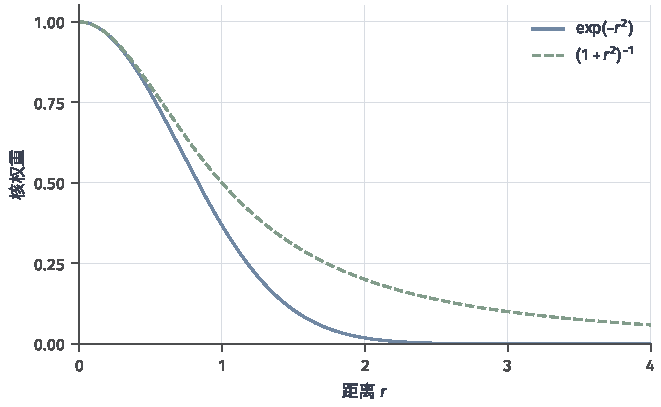
\includegraphics[width=105.412mm]{figures/04-classic-models/00-shared/matplotlib/dim-neighbor-tails/figure.pdf}
  \caption{高斯核$\exp(-r^2)$与Cauchy形核$1/(1+r^2)$的尾部。横轴$r$为无量纲距离，纵轴为未归一化核值，非概率密度、非实验结果；尾部形状本身不保证嵌入保真。}
  \label{fig:dim-neighbor-tails}
\end{figure}

\paragraph{收敛性}
坐标目标非凸，平移、旋转和反射也使坐标解不唯一。梯度光滑且步长合适时，可研究下降与趋近驻点；任意初始化的全局收敛仍无保证。即使谱方法全局解出固定图的子问题，图是否表达真实几何也要另行判断。

\paragraph{泛化性}

标准SNE输出一组训练坐标。处理新样本需另定邻域及旧坐标是否固定，并检验表示稳定性。输入距离若主要来自噪声，充分优化也可能只是保留这些噪声关系。

\subsubsection{小结}

SNE先以困惑度校准邻域，再以条件概率和KL散度学习坐标。表示能力、布局优化和点对计算各有约束：更换核、改进优化与计算加速分别解决不同问题，需要分别评价。

\subsection{t-SNE}
\label{sec:dim-tsne}

重尾核使较远位置仍保有相似度，为拥挤邻域提供更多布局余地。van der Maaten与Hinton于2008年提出\term{t-SNE}（t-distributed stochastic neighbor embedding），同时将逐点条件分布改为对称点对分布\scite{dim-vandermaaten2008tsne}这两项改变共同定义其目标。

\subsubsection{模型结构}

沿用高维条件概率与困惑度，为每对样本构造一个对称权重：
\begin{equation}
  \label{eq:dim-tsne-joint}
  \begin{aligned}
    p_{i,j}&=\frac{p_{j\mid i}+p_{i\mid j}}{2n},\qquad i\ne j,\\
    p_{i,i}&=0,\qquad p_{i,j}=p_{j,i},\qquad
      \sum_{i\ne j}p_{i,j}=1.
  \end{aligned}
\end{equation}
求和包括有序对的两个方向。$n$个条件分布各归一化为$1$，两方向相加后的总和为$2n$，因此分母取$2n$。若改按$i<j$求和，归一化及后续导数系数也需调整。

低维点对采用Cauchy形核，并在全部有序对上归一化：
\begin{equation}
  \label{eq:dim-tsne-low}
  \begin{aligned}
    u_{i,j}&=(1+r_{i,j}^2)^{-1},\qquad
      \mathcal{Z}=\sum_{a\ne b}u_{a,b},\\
    q_{i,j}&=\frac{u_{i,j}}{\mathcal{Z}},\qquad i\ne j,\\
    q_{i,i}&=0,\qquad \sum_{i\ne j}q_{i,j}=1.
  \end{aligned}
\end{equation}
$u_{i,j}$具有自由度为$1$的一维Student $t$核形状，$q_{i,j}$则是有限点对上的离散概率。重尾允许较远点获得相似度，未规定高低维距离相等，也未将$q_{i,j}$定义为$\mathbb{R}^k$上的多元Cauchy密度。

记$\bm{P}=(p_{i,j})$、$\bm{Q}=(q_{i,j})$，以点对分布间的KL散度学习坐标：
\begin{equation}
  \label{eq:dim-tsne-loss}
  C_{\mathrm{tSNE}}(\bm{Z})
    =\sum_{i\ne j}p_{i,j}\log\frac{p_{i,j}}{q_{i,j}}.
\end{equation}
全部点对共享归一化常数$\mathcal{Z}$。移动一个点会改变它和其他点的核值，也改变其余点对的概率，所以坐标要在共同概率预算下协调。

高概率近邻错置受到较大惩罚，簇间距离、面积和密度却未被要求复原。小$p_{i,j}$的吸引弱，但这些点对仍参与归一化与斥力计算，局部目标也需要考虑远点。

\subsubsection{参数学习}

代入低维核并利用$\sum_{i\ne j}p_{i,j}=1$，展开目标与归一化项的梯度：
\begin{equation}
  \label{eq:dim-tsne-gradient-derivation}
  \begin{aligned}
    C_{\mathrm{tSNE}}
      &=\text{常数}
        +\sum_{a\ne b}p_{a,b}\log(1+r_{a,b}^2)
        +\log\mathcal{Z},\\
    \nabla_{\bm{z}_i}\mathcal{Z}
      &=-4\sum_{j\ne i}u_{i,j}^2(\bm{z}_i-\bm{z}_j),\\
    \nabla_{\bm{z}_i}\log\mathcal{Z}
      &=-4\sum_{j\ne i}q_{i,j}u_{i,j}(\bm{z}_i-\bm{z}_j).
  \end{aligned}
\end{equation}
距离平方的导数贡献因子$2$，有序对的两个方向再贡献因子$2$。吸引项同理给出$4\sum_{j\ne i}p_{i,j}u_{i,j}(\bm{z}_i-\bm{z}_j)$，因此
\begin{equation}
  \label{eq:dim-tsne-gradient}
  \nabla_{\bm{z}_i}C_{\mathrm{tSNE}}
    =4\sum_{j\ne i}(p_{i,j}-q_{i,j})u_{i,j}
      (\bm{z}_i-\bm{z}_j).
\end{equation}
$p_{i,j}>q_{i,j}$时，负梯度拉近点对，反之推开。即使稀疏近似中$p_{i,j}=0$，有限距离的$q_{i,j}$仍为正，因而仍有斥力。每个点的位移由全部点对作用合成。

\term{早期夸大}（early exaggeration）在初始阶段将梯度中的$p_{i,j}$乘以$\alpha>1$，增强吸引后再恢复$\alpha=1$。原文使用$4$，后续也常用$12$，但需与学习率及样本数配合。夸大后权重和为$\alpha$，该阶段的更新已不是原归一化分布间KL散度的梯度。

初始化和动量也影响优化。缩放后的PCA坐标提供结构化起点，随机点云则不带这一信息；因此宏观布局差异可能同时来自起点与目标。动量未保证逃离局部极小值。实验应记录困惑度、学习率、初始化和夸大系数及轮数。

原始算法每轮需$O(n^2)$计算。Barnes--Hut t-SNE将吸引图稀疏化，并用低维树聚合远点、近似斥力，二维常用四叉树。固定近邻预算及近似精度、输出维数较小时，每轮典型成本为$O(n\log n)$；建图及极端布局仍会影响时间\scite{dim-vandermaaten2014accelerating}

FIt-SNE通过网格插值和快速傅里叶变换加速核求和\scite{dim-linderman2019fitsne}固定插值阶数时，斥力成本约为$O(n+g\log g)$，其中$g$为网格节点数，此外还需计算稀疏吸引。范围与精度改变时$g$也会改变。2019年工作展示了百万级单细胞数据的处理，实际规模与收益仍依赖计算条件。

\subsubsection{理论分析}
\label{sec:dim-tsne-theory}

\paragraph{表达能力}
重尾核缓解部分局部拥挤，输出维数和点对概率目标仍限制表示。视觉上分离的簇可能来自该目标的布局，原空间未必具有相同间距或密度。

\paragraph{收敛性}

坐标目标仍非凸。Linderman与Steinerberger在2019年SIAM期刊论文中，针对有适当簇结构的输入相似度、集中初始点云及满足条件的步长和夸大系数，分析早期簇内收缩与谱聚类的联系\scite{dim-linderman2019clustering}结论针对该阶段和条件，未覆盖任意数据的整个训练。

初始间距小时，$u_{i,j}\approx1$。若斥力扰动相对较小并暂不计动量，更新近似为
\begin{equation}
  \label{eq:dim-tsne-spectral-approximation}
  \begin{aligned}
    \bm{Z}^{(t+1)}
      &\approx(\bm{I}-4\eta_t\alpha\bm{L}_{P})\bm{Z}^{(t)},\\
    \bm{L}_{P}&=\bm{D}_{P}-\bm{P},\qquad
    (\bm{D}_{P})_{i,i}=\sum_{j\ne i}p_{i,j}.
  \end{aligned}
\end{equation}
对角矩阵$\bm{D}_{P}$记录行和。步长合适时，图平滑抑制快速变化方向，因而与拉普拉斯谱相联系。点云展开后，核值接近$1$的近似会减弱，斥力也更不可忽略；关闭夸大后，布局仍由两种作用共同调整。

\paragraph{泛化性}

困惑度决定输入分布，也决定所求问题。小值强调细邻域，可能割裂连续结构；大值引入更广关系，可能模糊稀有群体。可在可达范围内比较$5$、$30$、$50$等尺度及多次初始化，寻找稳定关系。不同困惑度对应不同目标分布，其KL值不能直接用于排名。

旋转和镜像通常不改变解释，簇间距、面积及疏密却也不能直接换算为原空间量。布局可能展开大簇、压紧小簇，或将连续变化分成区域。单细胞、文本或图像特征中的分组应回到合适的高维表示验证，并分别考察内部指标、稳定性、参考标签及下游效果（参见第\ref{sec:clustering-summary}节）。

新点需要额外扩展规则。openTSNE等实现固定参考坐标，再按新点与参考样本的相似度优化新坐标\scite{dim-policar2024opentsne}这是条件定位，与新旧样本联合训练不同；参考集未覆盖的新群体可能被安排到失真位置。

需要反复处理新样本时，可令$\bm{z}_i=f_{\bm{\theta}}(\bm{x}_i)$，按邻域目标学习共享参数。van der Maaten于2009年提出参数化t-SNE，以前向计算表示新点\scite{dim-vandermaaten2009parametric}网络函数族限制可实现布局，批次构造与归一化也影响训练关系。

\subsubsection{小结}

t-SNE用对称点对分布和重尾核组织局部相似性，适合探索邻域，却未建立全局距离的定量地图。加速算法降低计算成本，扩展规则方便定位新点；表示、优化与结构保真的限制仍需分别判断。

\subsection{UMAP}
\label{sec:dim-umap}

邻接关系也可以逐边赋予强度，无需使全部点对权重和为一。\term{统一流形逼近与投影}（uniform manifold approximation and projection，UMAP）先合并局部加权图，再优化低维连接强度。

McInnes、Healy与Melville自2018年公开的方法长文，将拉普拉斯特征映射、黎曼几何与模糊拓扑联系起来，讨论非均匀样本的局部度量及其合并\scite{dim-mcinnes2018umap}这一构造也面向较高维预处理。方法长文与同年JOSS软件论文分别描述理论构造和实现，几何解释、实现行为与可视化效果应各自评价。

\subsubsection{模型结构}

以$N_q(i)$表示不含$i$的$q$个近邻。先取互异样本、无并列最近邻及单位局部连接设置。记$\rho_i=\min_{j\ne i}\delta_{i,j}$，定义有向权重
\begin{equation}
  \label{eq:dim-umap-directed}
  \begin{aligned}
    v_{j\mid i}
      &=
      \begin{cases}
        \exp\!\left(-\dfrac{\max(0,\delta_{i,j}-\rho_i)}
        {\sigma_i}\right),&j\in N_q(i),\\
        0,&j\notin N_q(i),
      \end{cases}\\
    \sum_{j\in N_q(i)}v_{j\mid i}&=\log_2 q.
  \end{aligned}
\end{equation}
偏移$\rho_i$使最近邻权重为$1$，带宽$\sigma_i$控制其余边衰减。上述条件下，$q>2$时权重和随带宽从$1$趋向$q$，可搜索满足目标的带宽。距离可按任务更换，相应的几何解释也需要调整。

这些值是边的隶属强度，多条边可同时很强。校准目标$\log_2 q$未将行和设为$1$，也未使用熵或困惑度。重复或并列样本、其他局部连接设置可能使多条边固定为$1$，导致目标不可达，因而实现还需处理零距离、带宽下界与容差。

用模糊并将两个方向合成对称权重：
\begin{equation}
  \label{eq:dim-umap-union}
  v_{i,j}=v_{j\mid i}+v_{i\mid j}-v_{j\mid i}v_{i\mid j}.
\end{equation}
所得$v_{i,j}=v_{j,i}\in[0,1]$。一方向为$1$则合并为$1$，两方向均为$0.4$则合并为$0.64$。这是模糊集合运算，无需把两条边假定为独立事件。

\term{模糊单纯集}（fuzzy simplicial set）将点、边和三角面等组合结构赋予隶属强度，提供局部描述的组合框架。实际目标主要使用样本与加权边，即一维骨架。有限图中的环和空白是否对应真实拓扑，仍需采样与几何证据。

低维边强度由可调重尾核给出：
\begin{equation}
  \label{eq:dim-umap-kernel}
  w_{i,j}=\frac{1}{1+a r_{i,j}^{2b}},\qquad a>0,\quad b>0.
\end{equation}
由\code{min\_dist}和\code{spread}选择$a,b$，使光滑核逼近近处接近$1$、超过指定尺度后衰减的曲线。\code{min\_dist}允许控制紧凑程度，未给每对点施加硬距离下界。$a=b=1$时核形与t-SNE的$u_{i,j}$相同，但没有全局归一化，因而与$q_{i,j}$不同。

将每条边视为带软标签的二元判断，就可以匹配高低维边强度。按无序对$i<j$写完整目标：
\begin{equation}
  \label{eq:dim-umap-bernoulli}
  \begin{aligned}
    C_{\mathrm{B}}(\bm{Z})
      &=\sum_{i<j}\left[
        v_{i,j}\log\frac{v_{i,j}}{w_{i,j}}\right.\\
      &\qquad\left.+
        (1-v_{i,j})\log\frac{1-v_{i,j}}{1-w_{i,j}}
        \right].
  \end{aligned}
\end{equation}
该式求和逐边Bernoulli分布的KL散度。去掉只依赖高维权重的常数，得到二元交叉熵：
\begin{equation}
  \label{eq:dim-umap-cross-entropy}
  \begin{aligned}
    C_{\mathrm{CE}}(\bm{Z})
      &=-\sum_{i<j}\left[
        v_{i,j}\log w_{i,j}\right.\\
      &\qquad\left.+
        (1-v_{i,j})\log(1-w_{i,j})\right].
  \end{aligned}
\end{equation}
采用$0\log0=0$。两式对坐标有相同梯度，所以与t-SNE的核心区别在匹配对象：这里逐边二元匹配，t-SNE匹配全局归一化的点对分布。

正边项吸引，非边项排斥。$v_{i,j}=0$只说明局部图未保留这条连接，未区分稍远与极远的点对，因此该目标未规定全局距离保真。

\subsubsection{参数学习}

记吸引损失$\ell^+_{i,j}=-\log w_{i,j}$、排斥损失$\ell^-_{i,j}=-\log(1-w_{i,j})$。点对距离$r_{i,j}>0$时，其梯度为
\begin{equation}
  \label{eq:dim-umap-pair-gradient}
  \begin{aligned}
    \nabla_{\bm{z}_i}\ell^+_{i,j}
      &=\frac{2ab r_{i,j}^{2b-2}}
        {1+a r_{i,j}^{2b}}(\bm{z}_i-\bm{z}_j),\\
    \nabla_{\bm{z}_i}\ell^-_{i,j}
      &=-\frac{2b}
        {r_{i,j}^2(1+a r_{i,j}^{2b})}
        (\bm{z}_i-\bm{z}_j).
  \end{aligned}
\end{equation}
两项负梯度分别拉近与推开点对，完整目标再按$v_{i,j}$与$1-v_{i,j}$加权。接近重合时排斥项奇异，计算需稳定处理并控制更新幅度。

全点对计算仍为二次规模。\term{负采样}（negative sampling）按正边权重安排吸引，再为中心点抽$s$个排斥对象，抽样未逐个检查它们是否为非邻居。若图有$O(nq)$条边，每边每轮更新次数有界、$k$固定，一轮约需$O(nq(1+s))$；近似线性还要求$q,s$固定，并未包含建图和总轮数。

中心的更新频率取决于正边权重，负样本频率取决于采样分布。缺少重要性修正时，期望更新一般不同于完整交叉熵梯度，吸引与排斥的相对强度也随之改变。

Damrich与Hamprecht于2021年分析有效更新。令$\omega_i=\sum_{j\ne i}v_{i,j}$。在均匀负采样且排斥更新双端的模型下，略去共同正常数，有效目标为
\begin{equation}
  \label{eq:dim-umap-effective-loss}
  \begin{aligned}
    \widetilde C(\bm{Z})
      &=\sum_{i<j}\left[
        v_{i,j}\ell^+_{i,j}
        +\gamma_{i,j}\ell^-_{i,j}\right],\\
    \gamma_{i,j}&=\frac{s(\omega_i+\omega_j)}{2n}.
  \end{aligned}
\end{equation}
排斥系数由样本数、加权度和采样数决定，已不同于$1-v_{i,j}$。原文分析的非参数实现只移动排斥对的一端，其期望更新一般甚至没有对应的标量损失；上式仅适用于补上双端更新的版本\scite{dim-damrich2021umaploss}

暂将各$w_{i,j}$视为独立变量，其最优值为$v_{i,j}/(v_{i,j}+\gamma_{i,j})$。正边权重远大于排斥系数时，该值接近$1$，解释了部分紧凑布局倾向。实际坐标耦合全部边强度，未必能同时达到这些逐边最优值。

实现先搜近邻、估计尺度、合并图，再初始化并作采样更新。可取谱或随机初始化；断连分量之间缺少相对位置约束。学习率衰减、负样本数和排斥强度也影响布局，需与主要参数一起记录。

\code{n\_neighbors}控制连接尺度，较大值加入更广关系。\code{min\_dist}小允许紧凑群组，大则通常更分散，但这些变化未保证评价指标单调改善。\code{umap-learn}常用$q=15$、\code{min\_dist=0.1}作为起点；还需记录度量、维数、轮数、种子及版本\scite{dim-mcinnes2018umapsoftware}

\subsubsection{理论分析}
\label{sec:dim-umap-theory}

\paragraph{表达能力}
邻域图与距离约定选择关系尺度，输出维数限制可表达的连接强度。局部关系的近似匹配未要求全局等距，也未保证表示可逆或唯一。

\paragraph{收敛性}

完整交叉熵及有效采样目标都对坐标非凸，近邻近似、有限轮更新和梯度裁剪还会改变求解行为。趋近驻点的条件结论仅涉及给定目标，未保证最佳拓扑布局。负采样分析解释有效吸引与排斥，也未建立与非负矩阵分解的等价或相对t-SNE的普遍优势。

\paragraph{泛化性}

局部流形、尺度调整和模糊拼接说明图如何构造。有限样本结果仍依赖光滑几何、合适度量与足够采样；理论构造、近似建图和采样求解各有条件，不能直接将一层的保证用于另一层。

\code{transform}先在训练集找新点邻居，以邻居坐标初始化，再固定参考表示优化新点。这是给定参考图的条件定位。新数据接近训练分布时可借此放入同一图；新类别或分布漂移却可能使位置失真。

共享输入函数提供另一种扩展。Sainburg、McInnes与Gentner的参数化UMAP以正负样本训练网络，支持小批次和半监督学习\scite{dim-sainburg2021parametricumap}它通过前向计算处理新点，与固定参考图后优化位置不同；分布外泛化及对非参数布局的复现仍需验证。

子样本拟合后变换其余点可以节省计算，但子样本要覆盖稀有群体等重要关系。用于预测时，只在训练划分内拟合预处理和嵌入，再变换验证、测试数据，以免结构泄漏。表示的预测效用需直接评价。

\subsubsection{小结}

UMAP通过局部尺度与模糊并构图，以可调核布局并用采样降低计算量。边强度、完整匹配目标和有效更新各有含义。度量、建图、初始化及采样共同影响参考图与新点位置，应结合实际任务判断结果。

\subsection{模型对比与总结}
\label{sec:dim-manifold-comparison}
\label{sec:dim-neighbors-comparison}

表\ref{tab:dim-manifold-comparison}按输入、保留对象与求解比较六种方法。关系数据可以用于这些模型，但流形假设和谱求解并非共同前提：应力MDS通常迭代拟合。复杂度也应结合稠密矩阵、稀疏图或具体近似方案说明。

\begin{table*}[htbp]
  \centering
  \small
  \begin{tabularx}{\linewidth}{@{}>{\RaggedRight\arraybackslash}p{22mm}>{\RaggedRight\arraybackslash}X>{\RaggedRight\arraybackslash}X>{\RaggedRight\arraybackslash}X@{}}
    \toprule
    方法 & 输入与保留对象 & 核心求解 & 样本外使用与主要限制 \\
    \midrule
    MDS & 给定差异；经典型拟合内积，应力型拟合距离或顺序
      & 经典型取正谱；度量及非度量应力通常迭代求解
      & 需要到训练点的差异；非欧氏性与目标维数限制保真程度 \\
    核PCA & 正定核；特征空间方差
      & 中心化核矩阵的主特征方向
      & 核投影有明确公式；依赖训练中心化、核尺度和谱隙 \\
    Isomap & 邻域图；全局测地距离的估计
      & 最短路径后做经典MDS
      & 接入图后做距离扩展；短路、断连及不可展开几何会失真 \\
    LLE & 邻居与局部重构权；仿射重构关系
      & 局部线性方程与全局低端谱
      & 局部权重插值；病态邻域、多零模态与噪声需诊断 \\
    Laplacian Eigenmaps & 对称非负邻域权重；图上平滑性
      & 度加权广义特征值问题
      & 可作谱延拓；度、密度、断连影响低频表示 \\
    Diffusion Map & 对称权重及重加权；给定步数的扩散距离
      & 满足细致平衡的转移矩阵谱与时间加权
      & Nystr\"om延拓；截断、带宽和过度混合限制区分能力 \\
    \bottomrule
  \end{tabularx}
  \caption{六类方法在本节所述标准构造下的比较。MDS一行区分经典型与应力型，不能把二者的目标和求解混同。样本外一栏均指固定训练表示后的扩展，不代表加入新样本重新训练的等价结果，也不是预测性能保证。}
  \label{tab:dim-manifold-comparison}
\end{table*}

选择始于可信关系及误差含义。感知差异可用MDS，核PCA保留特征空间方差，Isomap适合有意义且可展开的长度结构。可信仿射关系对应LLE，图平滑对应拉普拉斯坐标，跨尺度概率连通对应扩散距离。分析动力系统时，还需让构图对应所研究的过程，才能将慢模态解释为相关慢变量。

\term{Hessian LLE}（Hessian特征映射）估计局部坐标函数的二阶变化，寻找其平方积分接近零的方向。连通且局部等距于欧氏区域等条件下，仿射坐标的Hessian为零；原理论允许某些非凸、带孔参数区域，但未涵盖任意带孔流形。估计二阶项还需足够且分布合适的邻居，采样要求通常比一阶拟合更强\scite{dimDonoho2003}

\term{局部切空间对齐}（local tangent space alignment, LTSA）在邻域中用PCA估计$m$维切空间及局部坐标，再令全局坐标经各邻域的仿射变换与其对齐。它显式利用局部线性结构，切空间估计与邻域选择的误差也会传到全局\scite{dimZhang2004}

\term{最大方差展开}（maximum variance unfolding, MVU）直接约束局部距离，优化未知Gram矩阵$\bm{B}$：
\[
  \begin{aligned}
    \max_{\bm{B}\succeq0}\quad&
      \operatorname{tr}(\bm{B}),\qquad \bm{B}\bm{1}=\bm{0},\\
    \text{满足}\quad&
      \bm{B}_{i,i}+\bm{B}_{j,j}-2\bm{B}_{i,j}
      =\lVert\bm{x}_i-\bm{x}_j\rVert_2^2,\quad(i,j)\in E.
  \end{aligned}
\]
中心化时，增大迹就是在保持局部边长下增大总方差。Gram矩阵上的问题是凸半正定规划，若再指定秩为$k$，则失去一般凸性。原问题的最优秩未必为$k$，截断后也可能违反局部距离约束；半正定求解本身还限制规模\scite{dimWeinberger2006}

\term{向量扩散映射}（vector diffusion maps）用邻域切空间间的正交对齐矩阵，使路径上的方向运输参与传播\scite{dimSinger2012}其连续对象是作用于向量场的连接拉普拉斯，补充了标量扩散没有直接表达的方向一致性。是否有益取决于任务所需信息。

这些方法各自约束不同对象。GPLVM用潜变量到观测的概率映射与似然学习坐标，t-SNE和UMAP用邻域目标布局，均不能一般化为给距离做经典MDS。概率邻域法与几何方法也分别适合不同目的，应按目标解释视觉分离与簇间位置。

非线性降维需要先选择可信关系，再判断目标维数能保留多少。核、邻域、归一化与时间尺度改变关系本身；求解正确、训练误差小、流形极限存在和下游有效，是四项需要分别核验的结果。

表\ref{tab:dim-neighbors-comparison}归纳三种邻域法的目标与边界。t-SNE困惑度为有效邻居数，UMAP的$q$为建图邻居数，两者均控制尺度，却不能直接换算。

\begin{table*}[tbp]
  \centering
  \small
  \begin{tabularx}{\linewidth}{@{}p{0.13\linewidth}>{\RaggedRight\arraybackslash}X>{\RaggedRight\arraybackslash}X>{\RaggedRight\arraybackslash}X@{}}
    \toprule
    比较方面 & SNE & t-SNE & UMAP \\
    \midrule
    高维对象 & 逐点条件邻居概率 & 对称联合点对概率 & 稀疏模糊邻域图权重 \\
    低维对象 & 行归一化高斯核 & 全局归一化重尾核 & 不作概率归一化的可调重尾权重 \\
    建模依据 & 条件分布匹配 & 点对分布匹配 & 局部几何与模糊图构造 \\
    优化目标 & 条件KL散度之和 & 联合KL散度 & 逐边交叉熵；负采样改变有效目标 \\
    邻域尺度 & 困惑度及逐点带宽 & 困惑度及逐点带宽 & 邻居数$q$、局部距离偏移和带宽 \\
    布局控制 & 初始化、学习率等 & 初始化、夸大、学习率等 & 初始化、核形状、采样和排斥等 \\
    迭代代价 & 稠密计算$O(n^2)$ & 稠密$O(n^2)$；树或插值可加速 & 固定嵌入维数下约$O(nq(1+s))$ \\
    全局解释 & 不保证距离或密度保真 & 簇间距、面积不宜直接解释 & 图连接提供约束，但不保证全局保真 \\
    收敛边界 & 非凸、依赖初始化 & 非凸；部分早期阶段有条件分析 & 非凸；依赖实际采样更新规则 \\
    新样本 & 需另定义扩展 & 参考图扩展或参数化版本 & \code{transform}或参数化版本 \\
    \bottomrule
  \end{tabularx}
  \caption{三种邻域降维方法。复杂度指固定嵌入维数下的一轮优化，不含建图和总轮数；$s$为每次正边更新的负采样数。}
  \label{tab:dim-neighbors-comparison}
\end{table*}

比较速度时应固定近邻搜索、近似精度、硬件、线程及优化预算，才能解释差异。预处理、初始化、版本与并行方式也影响复现。固定种子便于重跑，多种子和多尺度则用于检查结构稳定性。

% 将段落与其完整的会议文献边注安排在同一页内。
\Needspace{9\baselineskip}
LargeVis将可扩展建图与布局结合。Tang等人用随机投影树和邻居探索得到近似近邻图，再用概率图布局及负采样优化吸引与排斥\scite{dim-tang2016largevis}其目标另有定义，未无偏求解原SNE的条件KL。

% PaCMAP的长标题与作者列表也需留出边注空间。
\Needspace{10\baselineskip}
PaCMAP增加群组间位置的约束。Wang等人在近邻和远点对之外采中距离对，按阶段调整其权重以组织较大尺度关系\scite{dim-wang2021pacmap}实际效果还取决于配对、损失及初始化，实验指标改善需在相应数据范围内解释。

% 为该段及其较长的边注引文保留共同的页内空间。
\Needspace{9\baselineskip}
Amid与Warmuth于2019年提出TriMap，以三元组$(i,j,\ell)$要求$j$比$\ell$更接近$i$，并通过跨尺度采样与加权损失组织这些相对关系\scite{dim-amid2019trimap}结果保留所选排序，三元组与起点仍影响布局。

流形学习与邻域嵌入共享部分局部建图思路，选择时宜比较约束量、近似方式与目标。测地关系可用Isomap考察，相似样本的组织可用t-SNE和UMAP探索。用于下游特征时还可取$k>2$，按任务评价选择维数。

邻域嵌入优先表示重要邻接关系，图形因而可用于提出假设或展示已有分析支持的结构。簇数、大小与间隔仍需在原始或合适的高维表示中检验，并结合尺度、初始化及领域知识判断。经过这些核验，视觉关系才可成为分析证据。

\section{基于概率的降维}
\label{sec:dim-probabilistic}

概率降维先规定低维因素如何生成观测，再用观测推断这些因素。PPCA、FA与GPLVM分别改变映射、噪声或未知量的处理方式，均沿用$n,d,k$及输入矩阵$\bm{X}$。这一生成视角与第\ref{sec:classic-overview-probabilistic}节的潜变量建模相联系。

\subsection{概率主成分分析（PPCA）与因子分析}
\label{sec:dim-ppca}

多个传感器测量共同状态，却各有读数误差。区分共同变化与噪声，可以更明确地解释低维表示。\term{概率主成分分析}（probabilistic principal component analysis, PPCA）以低维高斯状态生成线性信号，再叠加同方差高斯噪声。

允许各观测坐标有不同噪声方差，就得到高斯\term{因子分析}（factor analysis, FA）。“因子”表示解释共同变化的潜变量。历史可追溯到Spearman于1904年的一般智力研究，现代多因子模型的含义和范围已不同于当时的心理测量假说\scite{spearman1904intelligence}

Tipping与Bishop在1999年为PCA引入与因子分析相关的概率模型，以似然刻画主子空间并研究EM估计\scite{tipping1999}在同一似然下，谱解与潜变量迭代可以比较，噪声及缺失观测也可以纳入统计推断。

\subsubsection{模型结构}
\label{sec:dim-ppca-structure}

令$\bm{z}\in\mathbb{R}^k$为潜变量，$\bm{W}\in\mathbb{R}^{d\times k}$为载荷，$\bm{\mu}\in\mathbb{R}^d$为均值。PPCA取$1\leq k<d$，以独立的潜变量和噪声生成观测：
\begin{equation}
\label{eq:dim-ppca-generative}
\begin{aligned}
\bm{z}&\sim\mathcal{N}(\bm{0},\bm{I}_k),\\
\bm{x}&=\bm{\mu}+\bm{W}\bm{z}+\bm{\epsilon},\\
\bm{\epsilon}&\sim\mathcal{N}(\bm{0},\sigma^2\bm{I}_d),
\qquad \bm{\epsilon}\perp\bm{z},\quad \sigma^2>0.
\end{aligned}
\end{equation}
各向同性约束噪声方向，观测的总方差仍可不同。给定潜变量时，条件负对数似然含平方残差$\lVert\bm{x}-\bm{\mu}-\bm{W}\bm{z}\rVert_2^2/(2\sigma^2)$；拟合边缘似然则还要将潜变量积分掉。

图~\ref{fig:dim-latent-model}区分两个方向：生成时抽取潜变量并加噪声，编码时给定观测求潜变量后验。
\begin{figure}[htbp]
  \centering
  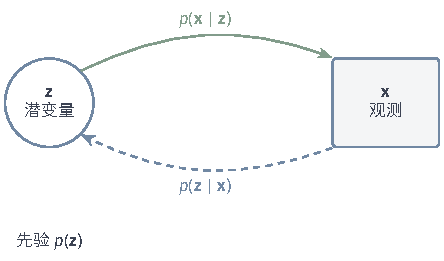
\includegraphics[width=75.188mm]{figures/04-classic-models/00-shared/tikz/dim-latent-model/figure.pdf}
  \caption{概率生成与后验推断的结构示意。实线表示$\bm{z}\to\bm{x}$的生成方向；虚线表示$\bm{x}\to\bm{z}$的后验推断，不是额外的生成依赖。图中节点与箭头只说明变量角色和条件关系，不表示实测数据、网络层数或计算流程；噪声描述观测对信号的偏离，不是新增的潜变量维数。}
\label{fig:dim-latent-model}
\end{figure}

独立高斯量线性组合仍为高斯量，将潜变量积分后得到
\begin{equation}
\label{eq:dim-ppca-marginal}
\begin{aligned}
p(\bm{x})&=\mathcal{N}(\bm{x};\bm{\mu},\bm{C}),\\
\bm{C}&=\bm{W}\bm{W}^\top+\sigma^2\bm{I}_d.
\end{aligned}
\end{equation}
信号协方差的秩至多为$k$，正噪声使$\bm{C}$正定；样本不足导致经验协方差奇异时，模型协方差仍可正定。

FA将噪声改为$\bm{\Psi}=\operatorname{diag}(\psi_1,\ldots,\psi_d)$，其中$\psi_j>0$为方差，故$\bm{C}=\bm{W}\bm{W}^\top+\bm{\Psi}$。给定因子，各维条件独立，跨维协方差由共同因子产生。独特方差也可包含特征自身的变化，解释时需结合测量机制；标准化会同时改变同方差假设的含义。

图\ref{fig:dim-ppca-fa-noise}固定载荷，只比较条件噪声。给定一个潜变量值，PPCA允许观测沿各方向等幅偏离均值，FA允许沿某坐标偏离更多。圆与椭圆均表示条件噪声；再混合不同潜变量值，才会加入信号协方差并形成总体分布。

\begin{figure}[htbp]
  \centering
  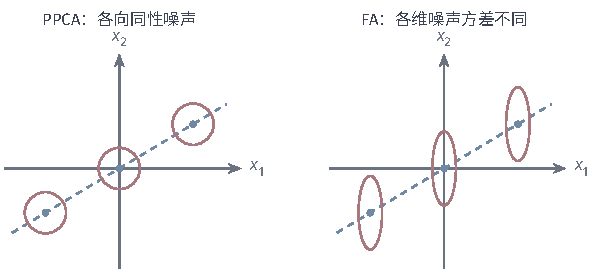
\includegraphics[width=101.840mm]{figures/04-classic-models/00-shared/tikz/dim-ppca-fa-noise/figure.pdf}
  \caption{PPCA与FA的条件噪声示意。设$d=2$、$k=1$、$\bm{\mu}=\bm{0}$、$\bm{W}=(1,0.6)^\top$，三个实心点对应$z=-1,0,1$的条件均值。左图取$\sigma=0.28$，右图取$\bm{\Psi}=\operatorname{diag}(0.16^2,0.50^2)$；每条轮廓到其中心的平方Mahalanobis距离均为$1$。坐标为无量纲构造值，轮廓是条件等密度线，不是总体数据云或置信区域。}
  \label{fig:dim-ppca-fa-noise}
\end{figure}

载荷的正交旋转$\bm{W}\bm{R}$不改变协方差。载荷满列秩且除旋转外局部可识别时，可扣除$k(k-1)/2$个旋转自由度：PPCA与FA的协方差参数数目分别为$dk+1-k(k-1)/2$及$dk+d-k(k-1)/2$，均值另有$d$个。FA还需排除载荷与噪声间的额外歧义。相较自由协方差的$d(d+1)/2$个参数，低秩约束可以降低估计方差，也可能带来模型偏差。

\subsubsection{参数学习}
\label{sec:dim-ppca-learning}

设样本独立同分布，均值为$\bar{\bm{x}}$，中心化量为$\bm{y}_i=\bm{x}_i-\bar{\bm{x}}$，记$\bm{S}=n^{-1}\sum_i\bm{y}_i\bm{y}_i^\top$。固定$\bm{C}$时，均值梯度$n\bm{C}^{-1}(\bar{\bm{x}}-\bm{\mu})$与负定二阶导数给出$\hat{\bm{\mu}}=\bar{\bm{x}}$。代回最大似然目标得
\begin{equation}
\label{eq:dim-ppca-likelihood}
\ell=-\frac{n}{2}\left[
d\log(2\pi)+\log|\bm{C}|
+\operatorname{tr}(\bm{C}^{-1}\bm{S})\right].
\end{equation}
对数行列式惩罚过大的协方差体积，迹项则惩罚在数据有较大变化的方向上赋予过小方差。

对$\bm{S}$作谱分解$\bm{U}\bm{\Lambda}\bm{U}^\top$，按$\lambda_1\geq\cdots\geq\lambda_d\geq0$排列。令$\bm{U}_k$包含前$k$个方向，$\bm{\Lambda}_k=\operatorname{diag}(\lambda_1,\ldots,\lambda_k)$。

证明需要比较两组谱的配对。Birkhoff--von Neumann分解说明：行和、列和均为$1$的非负方阵，即双随机矩阵，可以写成置换矩阵的凸组合\scite{birkhoff1946}因此双随机矩阵上的线性目标至少为某个置换取值的最小值。

最大似然解以PCA主方向构造载荷，以舍弃特征值的均值估计噪声，载荷内部保留旋转自由。下面先证明样本谱与模型谱同序配对最优，再优化谱值，从而说明全局最优性；奇异点及高维统计保证仍需另外讨论。

\begin{theorem}[PPCA的最大似然解]
\label{thm:dim-ppca-mle}
设$1\leq k<d$，尾谱均值$\tau=(d-k)^{-1}\sum_{j=k+1}^d\lambda_j$满足$\tau>0$且$\lambda_k>\tau$。在$\sigma^2>0$的PPCA模型中，以下参数达到全局最大似然：
\begin{equation}
\label{eq:dim-ppca-mle}
\begin{aligned}
\hat{\bm{\mu}}&=\bar{\bm{x}},\qquad
\hat{\sigma}^2=\tau,\\
\hat{\bm{W}}&=\bm{U}_k(\bm{\Lambda}_k-\tau\bm{I}_k)^{1/2}\bm{R}.
\end{aligned}
\end{equation}
其中$\bm{R}$为任意$k$阶正交矩阵。截断处有重根时，$\bm{U}_k$可在对应特征子空间内选取不同正交方向。
\end{theorem}

\begin{proof}
需最小化$F(\bm{C})=\log|\bm{C}|+\operatorname{tr}(\bm{C}^{-1}\bm{S})$。写$s=\sigma^2$，由信号半正定且秩至多为$k$，可行协方差的谱满足
\[
c_1\geq\cdots\geq c_k\geq s,\qquad
c_{k+1}=\cdots=c_d=s>0.
\]
允许$c_j=s$便包括载荷秩不足$k$的情况。

固定谱，设$\bm{p}_b$为$\bm{C}$的第$b$个单位特征向量，则
\[
\operatorname{tr}(\bm{C}^{-1}\bm{S})
=\sum_{a=1}^d\sum_{b=1}^d
\frac{\lambda_a}{c_b}(\bm{u}_a^\top\bm{p}_b)^2.
\]
平方内积构成非负且各行各列和为$1$的双随机矩阵，可写成置换矩阵的凸组合，所以上式不小于置换配对的最小值。若$\lambda_a\geq\lambda_b$、$c_a\geq c_b$，同序配对减去交换配对等于
\[
(\lambda_a-\lambda_b)
\left(\frac{1}{c_a}-\frac{1}{c_b}\right)\leq0.
\]
消去逆序配对即得$\operatorname{tr}(\bm{C}^{-1}\bm{S})\geq\sum_j\lambda_j/c_j$，取$\bm{p}_j=\bm{u}_j$达到等号。对数行列式只依赖谱，故同序对齐是固定谱下的全局最优。

对齐后，目标化为
\[
\begin{aligned}
F&=\sum_{j=1}^k\left(\log c_j+\frac{\lambda_j}{c_j}\right)\\
&\quad+(d-k)\log s+\frac{(d-k)\tau}{s}.
\end{aligned}
\]
暂去$c_j\geq s$及排序约束。对$a>0$，函数$g_a(v)=\log v+a/v$的导数为$(v-a)/v^2$，在$a$左侧为负、右侧为正，故$v=a$为唯一全局最小点。各首部项因此在$c_j=\lambda_j$处最小，尾部$(d-k)g_\tau(s)$在$s=\tau$处最小。

由$\lambda_k>\tau>0$，此解满足原约束。式~\eqref{eq:dim-ppca-mle}构造的协方差恰与$\bm{S}$同序对齐，首$k$个特征值为$\lambda_j$，其余为$\tau$，达到上述共同下界，故是全局最优。正交$\bm{R}$不改变载荷乘积；重根配对差为零，允许所述的不唯一性。
\end{proof}

边界情形要区分处理。$\lambda_k=\tau>0$时，同一公式仍给出最优协方差，但载荷降秩，满秩自由度与常规渐近分析不再直接适用。$\tau=0$时，样本协方差秩至多为$k$，未占据方向的方差可趋零使似然无界，正噪声模型中没有有限极大值。零噪声高斯分布奇异，已没有$d$维普通密度。

PPCA与PCA联系在主子空间，编码坐标还要由后验确定。生成模型的联合分布为
\begin{equation}
\label{eq:dim-ppca-joint}
\begin{bmatrix}\bm{z}\\ \bm{x}\end{bmatrix}
\sim\mathcal{N}\left(
\begin{bmatrix}\bm{0}\\ \bm{\mu}\end{bmatrix},
\begin{bmatrix}
\bm{I}_k&\bm{W}^\top\\
\bm{W}&\bm{C}
\end{bmatrix}\right).
\end{equation}
高斯条件公式给出后验均值$\bm{W}^\top\bm{C}^{-1}(\bm{x}-\bm{\mu})$与协方差$\bm{I}_k-\bm{W}^\top\bm{C}^{-1}\bm{W}$。记$\bm{M}=\bm{W}^\top\bm{W}+\sigma^2\bm{I}_k$，由$\bm{C}\bm{W}=\bm{W}\bm{M}$得到$\bm{W}^\top\bm{C}^{-1}=\bm{M}^{-1}\bm{W}^\top$，于是
\[
\bm{I}_k-\bm{M}^{-1}\bm{W}^\top\bm{W}
=\sigma^2\bm{M}^{-1}.
\]
将两项合并，后验写为
\begin{equation}
\label{eq:dim-ppca-posterior}
p(\bm{z}\mid\bm{x})
=\mathcal{N}\left(
\bm{M}^{-1}\bm{W}^\top(\bm{x}-\bm{\mu}),
\sigma^2\bm{M}^{-1}\right).
\end{equation}
在最大似然解中取$\bm{R}=\bm{I}_k$，后验均值的第$j$个坐标为
\begin{equation}
\label{eq:dim-ppca-score}
\mathbb{E}[z_j\mid\bm{x}]
=\frac{\sqrt{\lambda_j-\tau}}{\lambda_j}
\bm{u}_j^\top(\bm{x}-\bar{\bm{x}}).
\end{equation}
该坐标是PCA得分的缩放。再映回观测空间时，第$j$方向的系数为$1-\tau/\lambda_j$，而正交投影的系数为$1$。教学谱$(9,1,1)$取$k=1$，有$\tau=1$、载荷$\sqrt8\bm{u}_1$、后验方差$1/9$及重构系数$8/9$。

线性同方差假设使后验协方差不随完整观测值改变，它也未计入参数估计误差。固定满列秩载荷、令噪声趋零时，重构趋向列空间正交投影，潜在坐标仍受载荷尺度影响。

FA通常用迭代估计。\term{期望最大化}（expectation-maximization, EM）在E步求潜变量后验矩，在M步最大化完全数据对数似然的后验期望\scite{clust-dempster1977}“完全数据”包含观测与潜变量，是似然构造的对象，未表示潜变量已经测得。

各维均已观测时，可固定$\bm{\mu}=\bar{\bm{x}}$。第$t$轮E步计算
\begin{equation}
\label{eq:dim-fa-estep}
\begin{aligned}
\bm{V}^{(t)}
&=\left[\bm{I}_k+
(\bm{W}^{(t)})^\top(\bm{\Psi}^{(t)})^{-1}
\bm{W}^{(t)}\right]^{-1},\\
\bm{m}_i^{(t)}
&=\bm{V}^{(t)}(\bm{W}^{(t)})^\top
(\bm{\Psi}^{(t)})^{-1}\bm{y}_i,\\
\bm{Q}_i^{(t)}
&=\bm{V}^{(t)}+\bm{m}_i^{(t)}(\bm{m}_i^{(t)})^\top.
\end{aligned}
\end{equation}
$\bm{m}_i^{(t)}$、$\bm{V}^{(t)}$与$\bm{Q}_i^{(t)}$分别为均值、协方差与二阶矩。将它们汇总为
\[
\bm{A}^{(t)}=\frac1n\sum_i\bm{y}_i(\bm{m}_i^{(t)})^\top,
\qquad
\bm{B}^{(t)}=\frac1n\sum_i\bm{Q}_i^{(t)}.
\]
M步由这些统计量更新载荷及噪声：
\begin{equation}
\label{eq:dim-fa-mstep}
\begin{aligned}
\bm{W}^{(t+1)}&=\bm{A}^{(t)}(\bm{B}^{(t)})^{-1},\\
\bm{\Psi}^{(t+1)}
&=\operatorname{diag}\left[
\bm{S}-\bm{W}^{(t+1)}(\bm{A}^{(t)})^\top
\right].
\end{aligned}
\end{equation}
$\operatorname{diag}$保留对角元。将载荷正规方程代入期望残差协方差，就得到噪声更新，实际只需$\bm{S}$的对角。二阶矩必须包含后验协方差$\bm{V}^{(t)}$，否则会低估噪声。PPCA的EM则对各维残差方差再取平均。

可用PPCA载荷及正对角残差初始化，再交替两步。对角逆用除法，其他逆由线性方程求解。若约束$\psi_j\geq\varepsilon>0$并将更新截到下界，应明确这是受约束估计。停止诊断可用
\begin{equation}
\label{eq:dim-fa-stopping}
\begin{aligned}
r_\ell^{(t)}
&=\frac{|\ell^{(t+1)}-\ell^{(t)}|}{1+|\ell^{(t)}|},\\
r_C^{(t)}
&=\frac{\lVert\bm{C}^{(t+1)}-\bm{C}^{(t)}\rVert_{\mathrm{F}}}
{1+\lVert\bm{C}^{(t)}\rVert_{\mathrm{F}}}.
\end{aligned}
\end{equation}
两项残差连续若干步低于容差时停止，并设置最大轮数。协方差残差不受载荷旋转影响，达到轮数上限却仅表示预算耗尽。

\subsubsection{理论分析}
\label{sec:dim-ppca-analysis}

\paragraph{表达能力}
PPCA用低秩线性信号和同方差噪声约束协方差，FA增加各坐标的独特方差。线性、高斯及潜维数共同限制模型，多峰分布或非线性依赖需要其他生成形式。

\paragraph{收敛性}

条件满足时，PPCA谱解达到全局最大似然。FA的精确EM提高当前似然的相切下界，使似然不下降；有上界时似然值收敛。参数趋近驻点还需连续性与迭代有界等条件，全局最优仍无保证。弱因子与近零独特方差可能使更新缓慢。

\paragraph{泛化性}

统计分析先在去除载荷旋转的局部可识别坐标$\bm{\theta}$中进行。定义得分$\bm{s}_{\bm{\theta}}(\bm{x})=\nabla_{\bm{\theta}}\log p_{\bm{\theta}}(\bm{x})$。若支撑集不随参数变化，或相应边界项为零，且真参数邻域二阶可微、导数有可积包络允许交换微分与积分，则得分期望为零，并有
\[
  \bm{I}(\bm{\theta})
  =\mathbb{E}_{\bm{\theta}}\!\left[
      \bm{s}_{\bm{\theta}}(\bm{X})
      \bm{s}_{\bm{\theta}}(\bm{X})^{\top}
    \right]
  =-\mathbb{E}_{\bm{\theta}}\!\left[
      \nabla_{\bm{\theta}}^2\log p_{\bm{\theta}}(\bm{X})
    \right].
\]
这是Fisher信息的两种表达相等的正则条件\scite{vanderVaart1998asymptotic}参数化或边界破坏这些条件时，需重新核对恒等式。

一致性还要求真参数唯一最大化总体期望对数似然，并通过一致大数律及紧性或强制性控制样本最大点。渐近正态性进一步要求真参数为内点、二次均值可微、Fisher信息非奇异、局部似然有平方可积Lipschitz控制，且估计已经一致。模型正确、样本独立同分布、$d,k$固定并满足这些条件时，有
\[
  \sqrt{n}(\widehat{\bm{\theta}}_n-\bm{\theta}_0)
  \xrightarrow{\mathrm d}
  \mathcal{N}\!\left(
    \bm{0},\bm{I}(\bm{\theta}_0)^{-1}
  \right).
\]
正则条件的标准形式参见van der Vaart的M估计与光滑模型论述\scite{vanderVaart1998asymptotic}载荷旋转使原始矩阵不唯一；FA还要能区分低秩信号与对角噪声。参数数目不超过$d(d+1)/2$只是必要条件，仍需约束后的局部一一对应性及满秩导数。秩退化、零噪声或维数增长应另行分析。

较大$k$通常提高训练似然，模型选择因而还要考虑复杂度。常规正则模型可比较赤池信息准则（AIC）和贝叶斯信息准则（BIC）：
\[
\mathrm{AIC}=-2\hat{\ell}+2p,\qquad
\mathrm{BIC}=-2\hat{\ell}+p\log n,
\]
$p$包括均值和可识别协方差参数，准则越小越好。奇异点需其他证据近似或留出验证；普通PCA也可验证重构误差。所选$k$受噪声及用途影响，未必等于内在维数$m$。

若样本$i$只观测坐标集$O_i$，其似然使用已观测子向量的边际分布：
\begin{equation}
\label{eq:dim-linear-missing}
\bm{x}_{i,O_i}\sim
\mathcal{N}(\bm{\mu}_{O_i},\bm{C}_{O_i,O_i}).
\end{equation}
训练将各样本的边缘对数似然相加。E步只用$\bm{W}_{O_i,:}$与$\bm{\Psi}_{O_i,O_i}$，后验协方差随观测模式改变。M步按实际观测更新各维，或将缺失值和潜变量一并作为未观测量，求必要的一、二阶矩。

补全可用高斯条件均值，同时保留条件协方差或作条件采样以传播不确定性。若只填均值并视作真实观测，后续分析会低估误差。

忽略缺失机制通常需要\term{随机缺失}（missing at random, MAR）：给定已观测值，缺失概率不再依赖未观测值，且机制参数与数据参数可独立取值。若指标越严重越容易未被记录，仅用观测边缘似然仍可能有偏，需模型化缺失机制\scite{rubin1976missing}

概率模型把补全、表示与似然统一起来，PCA也可以构造其他补全方案。多个局部线性结构可进一步组成混合PPCA，其识别与退化需另查。

\subsubsection{小结}
\label{sec:dim-ppca-summary}

PPCA将主子空间置于最大似然框架，FA则允许异质独特方差，便于共同因子建模。两者在给定参数下都有后验与生成分布。PPCA编码是缩放后的主成分得分，FA的方向由因子模型决定，解释时要结合各自假设。

\subsection{高斯过程潜变量模型（GPLVM）}
\label{sec:dim-gplvm}

姿态或运动可以由少量状态控制，观测结构却未必线性。\term{高斯过程潜变量模型}（Gaussian process latent variable model, GPLVM）给低维到高维的函数设置先验，再从观测反求未知输入坐标。它与高斯过程回归共享核协方差及边缘似然计算；回归输入已知，本节输入也是待估计量（参见第\ref{sec:regression-gpr}节）。

Lawrence于2003年提出GPLVM，2005年系统论述其模型\scite{lawrence2005gplvm}推导从概率PCA的对偶表述出发，将载荷积分掉、转而估计潜在坐标，再以GP引入非线性函数先验。映射的不确定性被积分，坐标仍可作点估计，两者处理方式由此不同。

\subsubsection{模型结构}
\label{sec:dim-gplvm-structure}

\term{高斯过程}（Gaussian process, GP）规定有限输入处的函数值联合为高斯，核控制相关性与变化尺度。这里$\bm{X}$按训练均值中心化，生成时加回均值，$\bm{Z}\in\mathbb{R}^{n\times k}$按行存坐标。设
\begin{equation}
\label{eq:dim-gplvm-generative}
\begin{aligned}
f_j&\sim\mathcal{GP}(0,\kappa_{\bm{\theta}}),
\qquad j=1,\ldots,d,\\
x_{i,j}&=f_j(\bm{z}_i)+\epsilon_{i,j},
\qquad \epsilon_{i,j}\sim\mathcal{N}(0,\sigma^2).
\end{aligned}
\end{equation}
各输出函数独立并共享核参数$\bm{\theta}$，同一函数跨样本的值由核相关。噪声相互独立且独立于函数。非参数先验未预先限定固定有限基函数，核与噪声仍有待学习参数。

固定坐标并积分函数值。定义$\bm{K}_{i,h}=\kappa_{\bm{\theta}}(\bm{z}_i,\bm{z}_h)$及$\bm{C}_Z=\bm{K}+\sigma^2\bm{I}_n$，得到
\begin{equation}
\label{eq:dim-gplvm-likelihood}
\begin{aligned}
p(\bm{X}\mid\bm{Z})
&=\prod_{j=1}^d
\mathcal{N}(\bm{X}_{:,j};\bm{0},\bm{C}_Z),\\
\ell&=-\frac{nd}{2}\log(2\pi)
-\frac{d}{2}\log|\bm{C}_Z|\\
&\quad-\frac{1}{2}
\operatorname{tr}(\bm{C}_Z^{-1}\bm{X}\bm{X}^\top).
\end{aligned}
\end{equation}
$\bm{C}_Z$跨样本，为$n$阶；PPCA的协方差则跨观测维，为$d$阶。基本GPLVM优化$\bm{Z},\bm{\theta},\sigma^2$，保留坐标点估计。加独立标准高斯坐标先验后，目标多出$-\lVert\bm{Z}\rVert_{\mathrm{F}}^2/2$，最大后验估计仍只取坐标的一个值。

线性核$\kappa(\bm{z},\bm{z}')=\bm{z}^\top\bm{z}'$对应标准高斯载荷的线性函数先验。积分载荷并估计坐标，得到$\bm{C}_Z=\bm{Z}\bm{Z}^\top+\sigma^2\bm{I}_n$，称为\term{对偶PPCA}。它与PPCA交换积分和估计的对象，联合模型也随之改变。

对$\bm{G}=\bm{X}\bm{X}^\top/d$作谱分解，记有序特征值为$\rho_i$，前$k$个特征向量为$\bm{V}_k$，$\bm{D}_k=\operatorname{diag}(\rho_1,\ldots,\rho_k)$。无坐标先验惩罚，且$k<n$、$\eta=(n-k)^{-1}\sum_{i>k}\rho_i>0$、$\rho_k>\eta$时，同一谱证明给出
\begin{equation}
\label{eq:dim-gplvm-dual}
\begin{aligned}
\hat{\sigma}_{\mathrm{dual}}^2&=\eta,\\
\hat{\bm{Z}}&=\bm{V}_k(\bm{D}_k-\eta\bm{I}_k)^{1/2}\bm{R}.
\end{aligned}
\end{equation}
这里按$d$归一化，而PPCA按$n$归一化。左右奇异向量将两者联系到PCA，缩放、噪声估计及条件分布却不同。坐标先验改变目标后，也需重新求解。

平方指数、Matérn等核允许非线性生成，并规定相应平滑性。核选择限制可表达的函数。核PCA在已知观测上计算核，GPLVM在待学习坐标上计算核，二者核化的对象不同。

\subsubsection{参数学习}
\label{sec:dim-gplvm-learning}

坐标目标非凸，可用PCA初始化后，以L-BFGS或共轭梯度优化负对数似然。比较多次初始化时，固定训练划分与优化预算，考察最终对数似然。部分核有平移、旋转或坐标尺度与长度尺度的补偿对称，坐标解因而可能不唯一。

样本外检验时固定训练模型，遮住新样本的部分观测坐标，仅用其余坐标反求潜在位置，再计算被遮坐标的平均条件预测对数密度；值越大表示模型对这些未用于编码的观测赋予的密度越高。

微分行列式与逆矩阵，先得协方差梯度，再用链式法则传到参数：
\begin{equation}
\label{eq:dim-gplvm-gradient}
\begin{aligned}
\bm{H}&:=\frac{\partial\ell}{\partial\bm{C}_Z}\\
&=\frac12\bm{C}_Z^{-1}\bm{X}\bm{X}^\top\bm{C}_Z^{-1}
-\frac d2\bm{C}_Z^{-1},\\
\frac{\partial\ell}{\partial a}
&=\operatorname{tr}\left(
\bm{H}^\top\frac{\partial\bm{C}_Z}{\partial a}\right).
\end{aligned}
\end{equation}
$a$可表示坐标、核超参数或噪声方差，第二式将似然梯度传到具体未知量。

自动相关性确定（automatic relevance determination, ARD）为各潜在方向学习独立长度尺度。逆长度尺度平方$\alpha_r$控制该方向差异对相关性的作用。一个坐标同时改变核矩阵的行与列，求导需计入两者；正参数可在对数空间优化。

用Cholesky分解$\bm{C}_Z=\bm{L}\bm{L}^\top$代替显式求逆，以$2\sum_i\log L_{i,i}$计算对数行列式，用三角求解计算逆的作用。数值抖动用于稳定求解，应与统计噪声分别记录。

稠密分解需$O(n^3)$时间及$O(n^2)$存储，实际规模还受硬件与迭代数限制。稀疏GPLVM用$b\ll n$个\term{诱导点}及其函数值概括信息，将核心矩阵计算降为$O(nb^2+b^3)$，同时增加近似误差，输出与核计算另计\scite{lawrence2007sparse}

给定潜在坐标，GP条件分布可以预测观测，方差含函数不确定性与观测噪声。给定新观测要编码时，坐标仍未知，需要反求
\begin{equation}
\label{eq:dim-gplvm-encoding}
\hat{\bm{z}}_*=\argmax_{\bm{z}}
\left\{\log p(\bm{x}_*\mid\bm{z},\bm{X},\bm{Z})
+\log p(\bm{z})\right\},
\end{equation}
无先验版本删去先验项。反问题可能多解，需初始化或近似坐标后验。正向GP预测本身未给出直接编码器，学习反向映射属于额外扩展。

输出$j$只在$I_j$处观测时，用$\mathcal{N}(\bm{X}_{I_j,j};\bm{0},(\bm{C}_Z)_{I_j,I_j})$计算似然。各输出缺失模式不同，就不能共用一次完整分解。给定坐标可预测缺失值，但尚未传播坐标不确定性，仍需满足缺失可忽略条件。

Titsias与Lawrence于2010年提出\term{贝叶斯GPLVM}\scite{titsias2010gplvm}用变分分布保留坐标的不确定性，并优化对数边缘似然的\term{证据下界}（evidence lower bound, ELBO）：
\begin{equation}
\label{eq:dim-gplvm-elbo}
\begin{aligned}
q(\bm{Z})&=\prod_i\mathcal{N}(\bm{z}_i;\bm{\nu}_i,\bm{S}_i),\\
\log p(\bm{X})&\geq\mathcal{L},\\
\mathcal{L}
&=\mathbb{E}_{q(\bm{Z})}[\log p(\bm{X}\mid\bm{Z})]\\
&\quad-\operatorname{KL}(q(\bm{Z})\Vert p(\bm{Z})).
\end{aligned}
\end{equation}
均值$\bm{\nu}_i$与正定协方差$\bm{S}_i$为变分参数，KL表示Kullback--Leibler散度。将边缘似然写为$q$下的期望，再用Jensen不等式将对数移入期望，得到上述下界：期望对数似然衡量观测拟合，KL惩罚近似后验偏离先验。等价地，
\[
  \log p(\bm{X})-\mathcal{L}
  =\operatorname{KL}\bigl(q(\bm{Z})\Vert p(\bm{Z}\mid\bm{X})\bigr)
  \geq0.
\]
下界不超过对数边缘似然，二者差距为近似与真实坐标后验的KL散度；只有两种后验一致，差距才为零。

随机核矩阵的逆与行列式使第一项仍难积分。原方法借助诱导函数值再构造可计算下界，使适当核与高斯变分分布所需的期望有解析式。诱导点位置、核参数及噪声通常继续作优化变量，尚未对全部未知量作贝叶斯积分。

小$\alpha_r$表示核对该方向差异不敏感，可用于筛选有效方向。判断仍受先验、尺度、噪声及优化影响，也不能将筛选结果直接视为真维数。可在同一留出规则下比较预测对数密度，并将后验预测区间在留出观测上的覆盖率与标称概率对照，检查变分模型的预测和不确定性估计。

\subsubsection{小结}
\label{sec:dim-gplvm-summary}

GPLVM将生成函数的输入也视为未知。基本版本估计坐标并给出条件函数预测，贝叶斯版本近似坐标后验。姿态、运动或构象任务可以加入领域先验，同时需考虑核计算、局部最优及反向编码成本。

\subsection{模型对比与总结}
\label{sec:dim-probabilistic-comparison}

表~\ref{tab:dim-probabilistic-comparison}分别比较生成、学习与使用。噪声结构、映射形式及潜变量不确定性的处理是独立选择，需逐项核对。

\begin{table*}[htbp]
\centering
\small
\begin{tabularx}{\linewidth}{@{}>{\RaggedRight\arraybackslash}p{20mm}>{\RaggedRight\arraybackslash}X>{\RaggedRight\arraybackslash}X>{\RaggedRight\arraybackslash}X@{}}
\toprule
比较方面 & PPCA & FA & GPLVM \\
\midrule
生成映射 & 线性，共享各向同性噪声 & 线性，各观测坐标独立噪声 & GP函数先验；非线性取决于核，基本噪声为同方差高斯 \\
学习方法 & 正噪声非退化情形有谱解；也可EM & 通常用EM或其他数值优化 & 优化坐标和超参数；贝叶斯版本优化变分下界 \\
潜变量不确定性 & 给定参数时有精确高斯后验 & 给定参数时有精确高斯后验 & 基本版本为坐标点估计；需后验近似才能量化位置不确定性 \\
新观测编码 & 一次线性变换 & 一次线性变换 & 通常需反求新坐标，GP正向预测本身不是编码 \\
缺失观测 & 观测子协方差边际化 & 观测子协方差边际化 & 按输出的观测索引选取核子矩阵 \\
主要用途 & 线性压缩、去噪、受约束协方差估计 & 异质测量误差、共同因子建模 & 非线性生成关系、给定潜变量的输出预测 \\
\bottomrule
\end{tabularx}
\caption{概率降维模型比较。后验以固定参数为条件；GPLVM的函数预测方差不是潜在坐标方差。缺失值处理均要求正确边际化及可忽略的缺失机制。}
\label{tab:dim-probabilistic-comparison}
\end{table*}

完整稠密数据下，PPCA构造协方差并完整分解约需$O(nd^2+d^3)$，截断SVD或EM另有成本。FA利用对角噪声，每轮约为$O(ndk+nk^2+dk^2+k^3)$，总成本再乘轮数$T$。稠密GPLVM每轮通常为$O(n^3+n^2d+n^2k)$。比较时应同时规定$n,d,k$和求解器。

\term{混合PPCA}（mixture of PPCA）以非负且和为$1$的权重混合多个局部PPCA密度\scite{tipping1999mixture}像高斯混合模型一样，它引入成分变量和责任度，每个成分又有低秩信号及噪声。EM共同估计责任度与载荷，联系软聚类和局部降维（参见第\ref{sec:clustering-gmm}节）。局部坐标间的连续性尚需额外构造，分量坍缩与零噪声退化也需控制。

\term{贝叶斯PPCA}可给载荷列加分层先验，例如$\bm{W}_{:,r}\mid\beta_r\sim\mathcal{N}(\bm{0},\beta_r^{-1}\bm{I}_d)$。较大$\beta_r$压缩载荷，以ARD调整复杂度\scite{bishop1999bayesian}算法也可采用证据最大化，所选复杂度受模型与推断影响，未保证恢复真实维数。

观测类型还决定适合的分布。\term{指数族PCA}约束自然参数的低秩结构，以条件似然取代平方损失。泊松适合计数，伯努利适合二值，正连续数据可用满足参数域的Gamma观测。Collins、Dasgupta与Schapire的推广未必设置潜变量先验，因此还需区分低秩分解和完整生成模型\scite{collins2001exponential}

\term{变分自编码器}（variational autoencoder, VAE）用网络参数化观测分布，并让共享编码器输出近似后验，即摊销变分推断。高斯后验以均值加标准差逐元素乘标准高斯噪声重参数化，使采样进入下界梯度估计。它同时改变映射、推断和训练方式；相关神经表示入口参见第\ref{sec:neural-learned-representations}节\scite{kingma2013}

概率降维用生成假设解释误差，并组织编码与缺失值推断。线性信号可用PPCA或FA，非线性函数先验可用GPLVM；选择时要判断数据机制、预测目标及预算，并核对模型保留了哪些不确定性。

\section{模型选择与评价}
\label{sec:dim-evaluation}

\subsection{方法比较}

表\ref{tab:dim-selection}将保留目标对应到候选方法，表\ref{tab:dim-navigation}再补充映射及新样本处理方式。先确定用途，可以缩小需要比较的假设与误差。

\begin{table*}[!ht]
  \centering
  \small
  \begin{tabularx}{\linewidth}{@{}>{\RaggedRight\arraybackslash}X>{\RaggedRight\arraybackslash}X>{\RaggedRight\arraybackslash}X@{}}
    \toprule
    分析需求 & 可比较的方法 & 应检查的关键条件\\
    \midrule
    压缩、去相关与重构 & PCA、稀疏PCA & 尺度、解释方差、载荷稳定性\\
    分离低秩背景与污染 & RPCA及稳定变体 & 污染的稀疏形式、可识别性\\
    非负成分的加性解释 & NMF & 非负性含义、损失与成分稳定性\\
    少量原子的灵活组合 & 稀疏编码、字典学习 & 活跃原子数、推断成本\\
    流式与超高维预处理 & 随机投影 & 有限点集的距离失真与输出维数\\
    两个配对视图的共有信息 & CCA及正则化变体 & 配对质量、留出相关性\\
    线性混合信号的分离 & ICA & 源独立性、源数与噪声\\
    响应或类别相关的表示 & PLS、LDA、SIR & 监督信息仅在训练折使用，下游风险相对无监督与不降维基线\\
    只有距离或序数差异 & 经典、度量或非度量MDS & 距离可嵌入性、应力目标\\
    弯曲结构与几何分析 & 核PCA、Isomap、LLE、拉普拉斯特征映射 & 核、邻域、连通性与几何失真\\
    连通结构的多尺度分析 & 扩散映射 & 密度归一化、扩散时间与谱截断\\
    探索高维邻域结构 & t-SNE、UMAP & 邻域参数、初始化与重复运行\\
    缺失观测、噪声与生成建模 & PPCA、FA、GPLVM & 观测模型、缺失机制与后验近似\\
    \bottomrule
  \end{tabularx}
  \caption{按保留目标选择降维方法的起点。结果还应结合重构、邻域保持、样本外任务或预测分布评价；不同目标之间通常存在取舍。}
  \label{tab:dim-selection}
\end{table*}

方法的目标还要与映射形式配合。表\ref{tab:dim-navigation}将核PCA列为特征空间中的谱方法，将MDS列为差异到坐标的构造；几何展开与邻域布局均利用关系，但保留对象不同。各行因此提供比较属性，而非互斥分类。

\begin{table*}[!ht]
  \centering
  \small
  \begin{tabularx}{\linewidth}{@{}>{\RaggedRight\arraybackslash}p{21mm}*{5}{>{\RaggedRight\arraybackslash}X}@{}}
    \toprule
    代表方法 & 映射形式 & 保留对象 & 数据假设 & 样本外机制 & 下游用途 \\
    \midrule
    PCA、CCA、ICA；随机投影
      & 前三者从数据学习线性投影或解混；随机投影与数据独立抽取
      & 方差、跨视图相关、独立源或欧氏距离
      & 前三者分别假设低秩线性结构、配对视图或独立混合；随机投影无数据分布假设，JL保证只覆盖映射抽取前固定的有限点集
      & 共享矩阵直接变换
      & 压缩、去噪、多视图对齐、信号分离或高维预处理 \\
    NMF、稀疏编码
      & 线性生成字典；逐样本约束推断
      & 非负加性重构或稀疏支持
      & 非负观测或少量活跃原子
      & 固定字典后重新求系数
      & 部件解释、去噪与信号表示 \\
    经典MDS；核PCA
      & MDS由差异矩阵恢复谱坐标；核PCA由合法正定核定义特征空间谱坐标
      & MDS保留双中心内积及诱导距离；核PCA保留特征空间方差
      & MDS要求差异同尺度，欧氏差异对应半正定Gram矩阵；核PCA另要求核诱导几何适合任务
      & MDS扩展到训练点的差异；核PCA按训练中心化规则作核投影
      & 关系数据表示、非线性预处理与几何诊断 \\
    Isomap、LLE、拉普拉斯特征映射、扩散映射
      & 由训练图求非参数坐标
      & 测地距离、局部重构、图平滑或扩散距离
      & 可信邻域、充分采样及相应流形或图结构
      & 接入训练图后插值、距离扩展或谱延拓
      & 几何分析、多尺度连通性与后续建模 \\
    SNE、t-SNE、UMAP
      & 由邻域关系优化训练布局
      & 条件邻居概率、点对概率或模糊边权
      & 输入距离能表达局部相似性
      & 原始形式无共享函数；可作参考图变换或另学参数映射
      & 低维探索、局部结构展示与假设生成 \\
    PPCA、FA、GPLVM
      & 潜变量到观测的线性或核生成映射
      & 低秩协方差、异质噪声或非线性生成关系
      & 指定观测分布、噪声结构与核先验
      & 后验线性编码，或对新观测反求潜在坐标
      & 去噪、缺失值处理、生成建模与不确定性推断 \\
    \bottomrule
  \end{tabularx}
  \caption{降维方法的属性导航。各行给出本章标准形式的主要属性，而非互斥类别；具体变体可以改变映射、假设和样本外机制。}
  \label{tab:dim-navigation}
\end{table*}

随机投影的保证覆盖抽取映射前固定的有限点集，点集本身可以任意，无需指定来源分布。核PCA则要求核合法地表示特征内积；合法性与任务适用性是两个问题，还要用验证数据检查诱导相似关系。

\FloatBarrier
\subsection{评价与选择}

维数增长会使空间覆盖与统计估计更困难，这些现象统称\term{维数灾难}（curse of dimensionality）。每个单位坐标区间划成十段，$d$维空间就有$10^d$个区域，有限样本很快不足以覆盖。在部分弱相关分量组成的分布中，距离还会集中，近远样本的相对差异减小。现象依赖分布和度量；数据有冗余、低维结构或可提取的任务信息时，降维才可能缓解这些困难。

内在维数$m$描述给定尺度、噪声及结构假设下的局部自由度，表示维数$k$是按用途选择的输出规模。显示用的$k_{\mathrm{vis}}\in\{2,3\}$只反映画图限制，既未估计$m$，也未决定任务所需的$k$。

评价先规定用途与数据划分。均值、尺度、特征选择、投影、字典、核参数及邻域图均在训练折拟合；验证集选择方法与超参数，规则冻结后再报告独立测试结果。

若输出只有训练布局，探索结论仅针对固定样本。声称能处理新点时，要预先规定参考图扩展、插值或共享映射。表\ref{tab:dim-evaluation-protocol}将重构、距离、邻域、可视化、下游效用、稳定性及参数敏感性分别评价，并安排同一$k$、同一预算的简单基线。

邻域失真有两个方向：低维新增原来不近的邻居，或丢掉原来相近的邻居。固定同一批$n$个对象及两空间度量，令$N_i^{\mathrm{X}}(q)$、$N_i^{\mathrm{Z}}(q)$为各自$q$近邻，排除自身并以预定规则处理平局。平均重合率为
\[
  \frac{1}{nq}\sum_{i=1}^{n}
  \left|N_i^{\mathrm{X}}(q)\cap N_i^{\mathrm{Z}}(q)\right|.
\]
重合率只统计共同邻居的比例。\term{信任度}（trustworthiness）按原空间距离秩惩罚新增邻居，\term{连续性}（continuity）按低维距离秩惩罚丢失邻居，以区分错误程度。这里“连续性”是邻域指标的名称。

记$r_{i,j}$、$s_{i,j}$分别为$j$在$i$的原空间、低维距离秩，最近为$1$，最远为$n-1$。两类错误集合为
\[
  U_i=N_i^{\mathrm{Z}}(q)\setminus N_i^{\mathrm{X}}(q),
  \qquad
  V_i=N_i^{\mathrm{X}}(q)\setminus N_i^{\mathrm{Z}}(q).
\]
在整数$1\leq q<n/2$范围内，按最大秩罚分归一化：
\begin{equation}
  \begin{aligned}
    T(q)
      &=1-\frac{2}{nq(2n-3q-1)}
        \sum_{i=1}^{n}\sum_{j\in U_i}(r_{i,j}-q),\\
    C(q)
      &=1-\frac{2}{nq(2n-3q-1)}
        \sum_{i=1}^{n}\sum_{j\in V_i}(s_{i,j}-q).
  \end{aligned}
  \label{eq:dim-neighborhood-quality}
\end{equation}
$T(q)$为信任度，$C(q)$为连续性。此范围内，最远$q$个秩的超额总和为$q(2n-3q-1)/2$，因此两指标在$[0,1]$内，越大表示相应失真越少。结论限定于所选度量和$q$，语义正确与新点可靠性还需其他证据。

\begin{table*}[!htbp]
  \centering
  \small
  \begin{tabularx}{\linewidth}{@{}>{\RaggedRight\arraybackslash}p{23mm}>{\RaggedRight\arraybackslash}p{58mm}>{\RaggedRight\arraybackslash}X>{\RaggedRight\arraybackslash}X@{}}
    \toprule
    证据 & 测量与数据用法 & 基线或对照 & 不能单独替代 \\
    \midrule
    重构与压缩
      & 在验证或测试样本上报告与观测类型匹配的重构损失，并同时计算表示、模型或字典存储及编码、解码成本
      & 均值重构、同一$k$的PCA，以及不压缩的原始输入
      & 距离、判别信息或语义解释 \\
    距离保持
      & 对预先声明的点对报告相对失真、应力或秩相关；样本外主张须在训练映射未见过的数据上计算
      & 同一$k$的PCA或随机投影及原始距离
      & 邻域保持、可视化可信或下游风险 \\
    邻域保持
      & 在固定输入度量与邻居数下报告近邻重合率、信任度或连续性，并检查不同局部尺度
      & 原始空间邻域、同一$k$的PCA或随机布局
      & 全局距离、真实簇数或因果关系 \\
    可视化
      & 固定$k_{\mathrm{vis}}=2$或$3$，结合距离或邻域诊断、多次初始化和领域标注说明图上哪些关系可读
      & 二维或三维PCA、随机标签或与任务匹配的简单投影
      & 高维结构存在、簇语义正确或最佳预测表示 \\
    下游任务
      & 把降维器放入每个训练折，与后续回归、分类或聚类共同选择，在独立测试集报告相应风险或效用
      & 同一学习器使用原始表示、简单PCA和任务允许的特征选择
      & 几何保真、生成假设正确或解释可靠 \\
    稳定性
      & 改变训练样本、初始化和随机种子；在共同样本上比较对齐坐标、距离或邻域，线性模型还可比较投影子空间，再检查下游结论是否保持
      & 算法自身多次运行及确定性基线
      & 统计正确性；稳定的偏差仍可能重复出现 \\
    参数敏感性
      & 在预先给定范围内改变$k$、邻居数、核带宽、困惑度或正则强度，报告结论在哪些范围保持
      & 默认参数、简单尺度规则和等预算搜索
      & 独立测试；用测试集挑参数会使其失去最终证据资格 \\
    \bottomrule
  \end{tabularx}
  \caption{降维的统一评价协议。各类证据回答不同问题；训练目标低、二维图清晰或单次下游得分高，都不能替代其余证据。}
  \label{tab:dim-evaluation-protocol}
\end{table*}

维数可在同一数据协议下分步选择：
\begin{enumerate}
  \item 声明用途与保留对象，据此选择重构、距离、邻域、可视化或任务风险作为主要证据。
  \item 在训练折拟合尺度和表示，再以局部谱、邻域尺度、重构曲线或内在维数估计形成$m$及候选$k$的依据。这些估计受尺度和假设影响。
  \item 在验证集联合选择$k$、核、邻居数和正则强度。交付图形时另设$k_{\mathrm{vis}}$，并用较高维候选及表\ref{tab:dim-evaluation-protocol}的诊断量检查显示引入的失真。
  \item 冻结预处理、映射、$k$、新点机制及评价规则，再在独立测试集报告结果。若根据测试结果继续改维数，应另取测试证据。
\end{enumerate}

可先以PCA或随机投影压缩，再做非线性嵌入，但要检查前一步是否保留所需结构，“保留50维”仅是经验起点。预测用途应将降维器与后续模型一同训练、验证，再用独立数据比较风险（参见第\ref{chap:regression}、\ref{chap:classification}章）。聚类用途还需在原特征或已验证表示中检查稳定性及外部证据（参见第\ref{chap:clustering}章）。显示维数另行选择，不必限制部署表示的维数。

\Needspace{18\baselineskip}
\section{本章小结}
\label{sec:dim-summary}

降维以较少坐标保留所需信息。线性及核方法提取全局变化，距离法拟合点对差异，邻域法组织局部关系，概率法解释低维因素的生成作用。方差、距离、重构与预测收益各有指标，维数减少本身尚未说明目标已达到。

选择还要区分内在自由度、任务表示规模与显示维数，核对新点编码、不确定性及计算代价。二维图可提出假设，结构与预测价值则需要相应证据验证。

回归和分类中的表示应与预测模型在同一训练验证流程中选择，以独立数据评价风险。聚类中的表示还改变距离，需要检验群组证据。方法假设与评价匹配，才能说明哪些信息确实被保留。

\paragraph{扩展阅读}
Bishop教材第12章介绍连续潜变量与PCA的概率解释，可进一步理解生成模型和几何压缩的联系。Hastie等的教材讨论非线性表示与预测，可对照本章分别检验重构、邻域和任务风险\scite{bishop2006,hastie2009}
